\documentclass[./main_en.tex]{subfiles}
\graphicspath{{\subfix{./figs}}}

% ------------ main document ------------ 
\begin{document}
\chapter{\chapEcoEn} \label{chap:ecoeco}

% custom paragraph skip
\setlength{\parskip}{0mm}

\epigraph{\small{When I worked at the World Bank, I often heard the statement: \say{There is no conflict between economy and ecology. We can and must grow the economy and protect the environment at the same time}. I still hear this often today.}}{Herman Daly (2015, p. 1) \cite{Daly2015a}}

\epigraph{\small{We can break our dependence on fossil fuels, excessive consumption, and the current development model by creating a more sustainable and desirable future. It will not be easy; it will require a new vision, new measures, and new institutions. It will require a directed evolution of our entire society. But breaking this dependence is not a sacrifice of quality of life. On the contrary, it is a sacrifice not to do so.}}{Robert Costanza (2016, p. 23) \cite{potschin2016}}


% custom paragraph skip
\setlength{\parskip}{\myparskip}

\section{Choosing an economic paradigm} \label{chap:ecoeco:sec1}

\par In the previous chapter, I explored the evolution of Hydrology throughout the 20th century, which has rapidly shifted paradigms since the advent of the International Hydrological Decade in the 1960s, arriving today at an era that acknowledges the diversity of hydrological processes, especially in zero-order basins. Furthermore, the use of hydrological models has also become more critical and aware of its limitations, reflecting the advance of the instrumentalist approach which, in the absence of complete information about the target system, accepts multiple empirically adequate realizations and the treatment of associated uncertainties. This trajectory raises a fundamental question for water resources management: how can this sophisticated theoretical and practical knowledge offered by Hydrology be applied to enhance the integrated management of water resources?

\par In the context we find ourselves in, where water resource management aims to ensure society's water security, an inevitable confluence with Economics — the science of allocating scarce resources — emerges. This challenge becomes even more critical in the face of climate change, which this year (2024) manifested alarmingly in various parts of the world, revealing society's vulnerability to extreme weather events. Simultaneously, recent initiatives in Brazil, such as the National Program for Watershed Revitalization, the National Policy for Payments for Environmental Services, and the consolidation of ANA's Water Producer Program, signal a movement being nurtured by federal institutions, creating momentum for other Union members and sectors as well. Therefore, more than a superficial application of hydrological models is needed. On the contrary, it becomes essential to deeply understand the \textbf{economic paradigm} that will guide these decisions. Only then will it be possible to advance in the use of hydrological knowledge and modeling techniques to design management policies that respond both to the demands of an uncertain climate context and the need to rationally allocate our natural resources.

\par Although this chapter advances to a more applied sphere, aimed directly at supporting water resource management, it will be necessary to take a few steps back and explore fundamental philosophical questions. This digression, however extensive it may seem, is indispensable to grounding the use of hydrological models within \textbf{Ecological Economics} — the economic paradigm that embodies both the concept of \say{sustainable development} and the concept of \say{environmental or natural services}. From this understanding, we can more deeply interpret what it means to regenerate or conserve natural services in watersheds. In particular, we will see that to reach the application of models, I will need to scale a stack of concatenated concepts, from abstract ethical principles to the mapping of priority rural plots for green infrastructure expansion. In relation to the landscape analogy I have developed so far, if in the previous chapter we entered an open and tangible terrain, where rivers flowed abundantly, here the rivers enter avulsion, creating vast swamps as labyrinthine as the mountain tops. With some patience, however, it is possible to reach the sea.

\section{Between means and ends: Economics} \label{chap:ecoeco:economy}

\begin{figure}[t!] 
\centering				
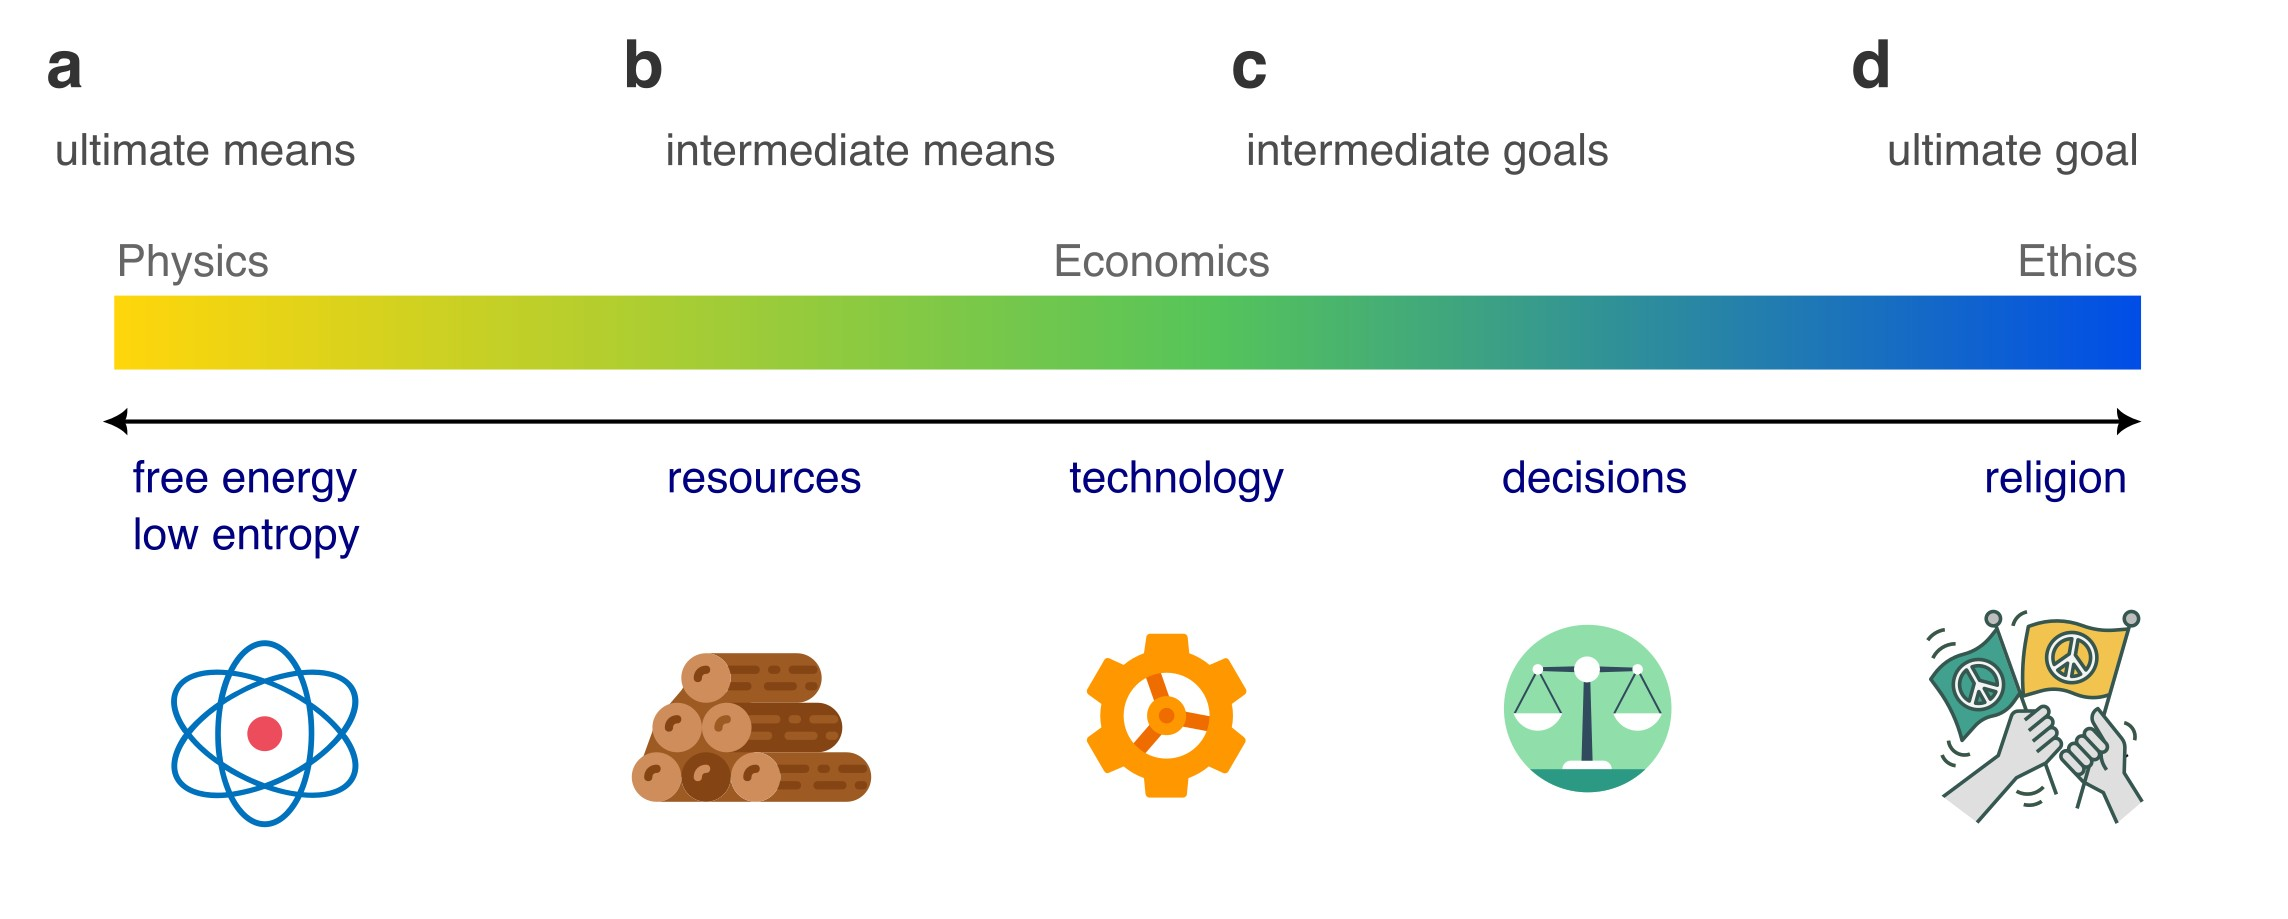
\includegraphics[width=0.98\linewidth]{figs/fig_economics_en.jpg}		
\caption[The Spectrum of Economics]
{\textbf{---\;The spectrum of \gls{gseconomics}.}
    Economics, as the allocation of scarce resources among different goals, connects resources (means) and objectives (ends). \;\textbf{a}\;---\;Free energy and low-entropy materials are the ultimate means.
    \;\textbf{b}\;---\;Energy and materials manifest through intermediate means: natural resources and resources transformed by technology.
    \;\textbf{c}\;---\;Decisions based on the application of technology guide the allocation of intermediate resources to meet intermediate goals.
    \;\textbf{d}\;---\;Decisions are oriented by some religion, a set of ethical values aimed at a supreme goal, whether explicit or not.}
\label{fig:eco:economics} 		
\end{figure}

\par \textbf{\gls{gseconomics}} is the science dedicated to studying the allocation of scarce resources among different objectives. For example, we might choose to use steel to build houses or missiles; allocate water for agricultural irrigation or energy generation; use land to maintain standing tropical forests or to raise and slaughter cattle. What is the best option? If these resources are truly scarce, these options are not mere fallacious false dichotomies but very serious questions, with drastically different consequences depending on the choice. In this sense, \gls{gseconomics} is not only associated with the existence of scarce resources but is also intrinsically linked to the \textbf{decision-making} process, as choices must be made because we cannot have everything simultaneously. This raises the following central question:

-- What are the objectives that guide choices?

\noindent This is clearly not an empirical question. It cannot be answered by undertaking a field expedition and testing hypotheses against observed evidence, as scientific questions are. In this case, the empirical world would simply offer a confusion of contradictory answers. Nor is it a Logical question, which could be answered from fundamental axioms, as in Geometry. The question, therefore, reveals itself to be essentially \textbf{\gls{gsethics}}: it presupposes a moral value of what \textit{should} be aimed at\footnote{This type of question is also known as \textbf{normative}.}. \gls{gsethics} is the branch of Philosophy that explores the principles and values guiding human behavior, seeking to define what is considered right or wrong, just or unjust, what should and should not be done. Therefore, the central question of \gls{gseconomics} depends on an ethical orientation, making this science a bridge that connects means (resources) with ends (objectives), as illustrated in Figure \ref{fig:eco:economics}. In the strict realm of Biology, of course, all organisms must deal with the allocation of scarce resources to address the \textbf{\gls{existimper}}, which has nothing to do with \gls{gsethics}. This imperative consists of a clear objective: to exist, one must make decisions to \textit{continue} existing. Thus, the \gls{ultimategoal} of a living being is to metabolize and reproduce, by definition. In human terms, this implies obtaining the minimum conditions for survival, such as food, water, clothing, hygiene, physical shelters, and, above all, social relationships.

\par Unlike other living beings, historian Yuval Harari suggests that \textit{Homo sapiens} instantiate \textbf{religions} that define existential goals beyond mere survival \cite{harari2015sapiens}. Religions are collective fictions, intersubjective realities that exist only in the shared imagination among people of a given group. In this sense, religions define the ethical framework by which humans guide their choices. The historical processes of the Renaissance and Modernity gave rise to \textbf{\gls{gshumanism}} in Western Europe, a religion that is widely influential today. In contrast to earlier religions that worshiped supernatural entities, \gls{gshumanism} is expressed as a form of \textbf{\gls{antropoc}}, as it centers on the human being as the focal point of all our objectives \cite{lamont1997philosophy}. An example of the transformation implied by \gls{gshumanism} can be found in René Descartes' \textit{Discourse on the Method}, where the philosopher proposes that the pursuit of truth should go beyond a theoretical understanding of reality to find practical applications that improve human conditions \cite{descartes2008discurso}. In the medieval mindset, however, this conception was inaccessible, as knowledge aimed to understand God's work, and the miserable human condition would be saved only after death. Other religions eventually assume that our misery is related to reincarnations, etc. Through a political lens, \gls{gshumanism} gave rise to various sub-religions, or doctrines, such as Liberalism, which worships the \say{individual}, Socialism, which worships \say{society}, and Fascism, which worships the \say{nation}\footnote{These doctrines are obviously not rigid, existing on a gradient and featuring unusual combinations with one another and with other traditional religions. For example, Socialism may be influenced by Liberalism, as seen in the European Union, or by Fascism, as seen in the Soviet Union.}. But primarily, \gls{gshumanism} also gave rise to modern \textbf{\gls{gnaturalism}}, a \gls{teoria} grounded in realism that asserts that nothing exists outside the natural world and, therefore, any explanation of reality must be found within the Universe itself.

\subsection{The ethics of Utilitarianism} \label{subsec:bentham}

\par In the field of \gls{gsethics}, a philosophical branch within \gls{gshumanism} is Jeremy Bentham’s \textbf{\gls{gutilitarism}} (1748-1832) \cite{Gordon2002a}. This philosopher proposes that the morality of an action should be determined by its consequences, focusing on maximizing the \textbf{\gls{welbeing}} of the largest number of individuals possible. For Bentham, the fundamental principle guiding moral evaluation is \textbf{\gls{gutility}}, understood as an action's capacity to increase or decrease the pleasure and pain of those affected by it. Bentham defines \gls{welbeing} as the predominance of pleasure over pain and argues that all human actions are motivated by these two factors. He develops an evaluation method known as the \textbf{\gls{hedonacc}}, which allows for measuring the moral impact of an action by considering aspects such as intensity, duration, certainty, proximity, and extent of the pleasures and pains involved. This calculation aims to quantify the well-being generated by actions and guide moral choices. Bentham’s \gls{gutilitarism} thus adopts a consequentialist and impartial perspective, where the correctness of an action depends on its practical outcomes rather than the agent's intentions. Additionally, this \gls{teoria} considers that the well-being of all affected should be weighed equitably. Thus, the morally correct action is the one that promotes the maximum pleasure and minimum pain for the largest number of people, serving as the ultimate metric for judging the moral value of actions.

\par From a distance, Bentham’s \gls{gutilitarism} makes sense. Within \gls{gshumanism}, the idea of maximizing \gls{welbeing}, of guiding decisions to avoid pain and seek pleasure, is intuitive and natural. However, this ethical \gls{teoria} is vague enough to allow for diverse interpretations, leading to very different political and economic orientations in practice. Theoretically, Liberalism, Socialism, and Fascism are utilitarian in one form or another, though the materialization of their ideas during the 20th century resulted in vastly different economies and political regimes. In Liberalism, the premise is that if each individual is free to maximize their own well-being, the overall well-being will increase through a kind of self-regulation. In Socialism, it is assumed that collective well-being will grow through State regulation or management of the economy. In Fascism, it is believed that the general well-being of the nation will be maximized as long as individuals or groups considered traitors or impure are expelled (or worse).

\par To complicate matters, \gls{gutilitarism} faces challenges with a very fragile scientific foundation. Modern psychological and neurological theories suggest that it is impossible to indefinitely amplify a subjective sensation. \textbf{\gls{adaplevel}}, for instance, establishes that constant emotional stimuli shift to a mental background where they are then ignored, freeing mental resources to adequately process \textit{novelties} \cite{Edwards_2018}. Along these lines, the pursuit of more well-being leads humans into a \textbf{\gls{hedonmill}}, a form of chronic and addictive existential dissatisfaction where, even with constant improvements in material comfort and rewarding experiences, the level of well-being tends to return to a fixed baseline, frustrating the search for lasting and increasing happiness \cite{Diener2009}. Empirical evidence supports this thesis, such as in situations where lottery winners (a positive event) and individuals disabled by accidents (a negative event) return to their baseline level after the event \cite{Brickman_1978}. Since neuroscience supports that pain and pleasure are fundamentally material processes (synapses), these psychological and physiological states cannot grow indefinitely, complicating the idea of \say{maximizing human well-being}\footnote{Neuroscience establishes that thoughts are synapses. Without synapses, thoughts do not exist. However, neuroscience does not explain the \textit{subjective manifestation} that accompanies synapses. This is known as the \gls{consproblem}.}.

\par \gls{gseconomics} has deeply incorporated the concept of maximizing \gls{gutility} as its \textbf{\gls{ultimategoal}}, which underpins both \textbf{\gls{microeon}}, focused on explaining the functioning of specific markets and the interactions between consumers and producers, and \textbf{\gls{macroeon}}, which seeks to understand the economy as a whole, from the national level to the global economy. However, the classical doctrines of these theories, developed in the 19th century, although scientific, struggled to sustain themselves empirically over time. Theorists began questioning their fundamental assumptions as early as the 19th century, and these critiques intensified throughout the 20th century. In \gls{microeon}, the classical version was revised by modern approaches such as \textbf{Evolutionary Microeconomics}, which expands classical concepts by introducing bounded rationality, dynamic behavior, and institutional interactions \cite{Nelson1985a, Bourgine2006a}. This approach aims to explain more complex and realistic phenomena, such as price dispersion and the diversity of industrial structures, which classical \gls{teoria}, based on perfect rationality and static equilibrium, found challenging to address.

\par Another transformation of substantial importance in \gls{microeon} was the advent of \textbf{Environmental Economics}\footnote{Also called Neoclassical Environmental Economics, to denote its distinction from Ecological Economics}. According to Pearce (2002) \cite{Pearce2002a}, this microeconomic school originated in the 1950s in the United States with the creation of \textit{Resources for the Future} (RFF). This institution was dedicated to investigating issues related to the scarcity of natural resources and their economic impacts. According to the author, the 1960s were marked by a strengthening of this discipline, driven by the environmental movement, notably through works such as \textit{Silent Spring} (1962) by Rachel Carson and \textit{Spaceship Earth} (1966) by Boulding. This context led economists to delve deeper into the study of \textbf{externalities} — unpriced impacts of economic activities on third parties — based on theoretical foundations such as those developed by Pigou (1920). Pearce highlights that, building on these foundations, economists began employing cost-benefit analyses to underpin environmental public policies, using concepts such as the Kaldor-Hicks compensation criterion. With this advancement, the traditional separation between natural resource economics (focused on the optimal use of resources) and environmental economics (centered on pollution) began to blur. This occurred particularly with the incorporation of economic growth theories that accounted for environmental limits. Additionally, numerous contributions emerged on how to address externalities, proposing solutions such as taxes, regulations, or private negotiations. These approaches fostered market-aligned environmental policies. Thus, Environmental Economics established itself as a subdiscipline of Neoclassical Microeconomics, integrating theories of economic welfare, sustainable growth, and instruments such as pollution taxes and tradable permits to promote economic efficiency and environmental sustainability. Despite its practical nature regarding natural resource management instruments, this school does not challenge the broader understanding of \gls{macroeon}. On the other hand, proponents of \gls{ecoeco}, such as Herman Daly (1938–2022), completely reject the classical and neoclassical \gls{macroeon} doctrine, arguing that it overlooks the laws of thermodynamics. As we will see later, \gls{ecoeco} proposes a genuine \gls{paradigma} shift, placing sustainability at the center of macroeconomic analyses and emphasizing that unlimited \gls{ecogrowth} is unfeasible on a planet with finite resources.


\subsection{The Theory of Marginal Utility} \label{subsec:marginutil}

\begin{figure}[t!] 
\centering				
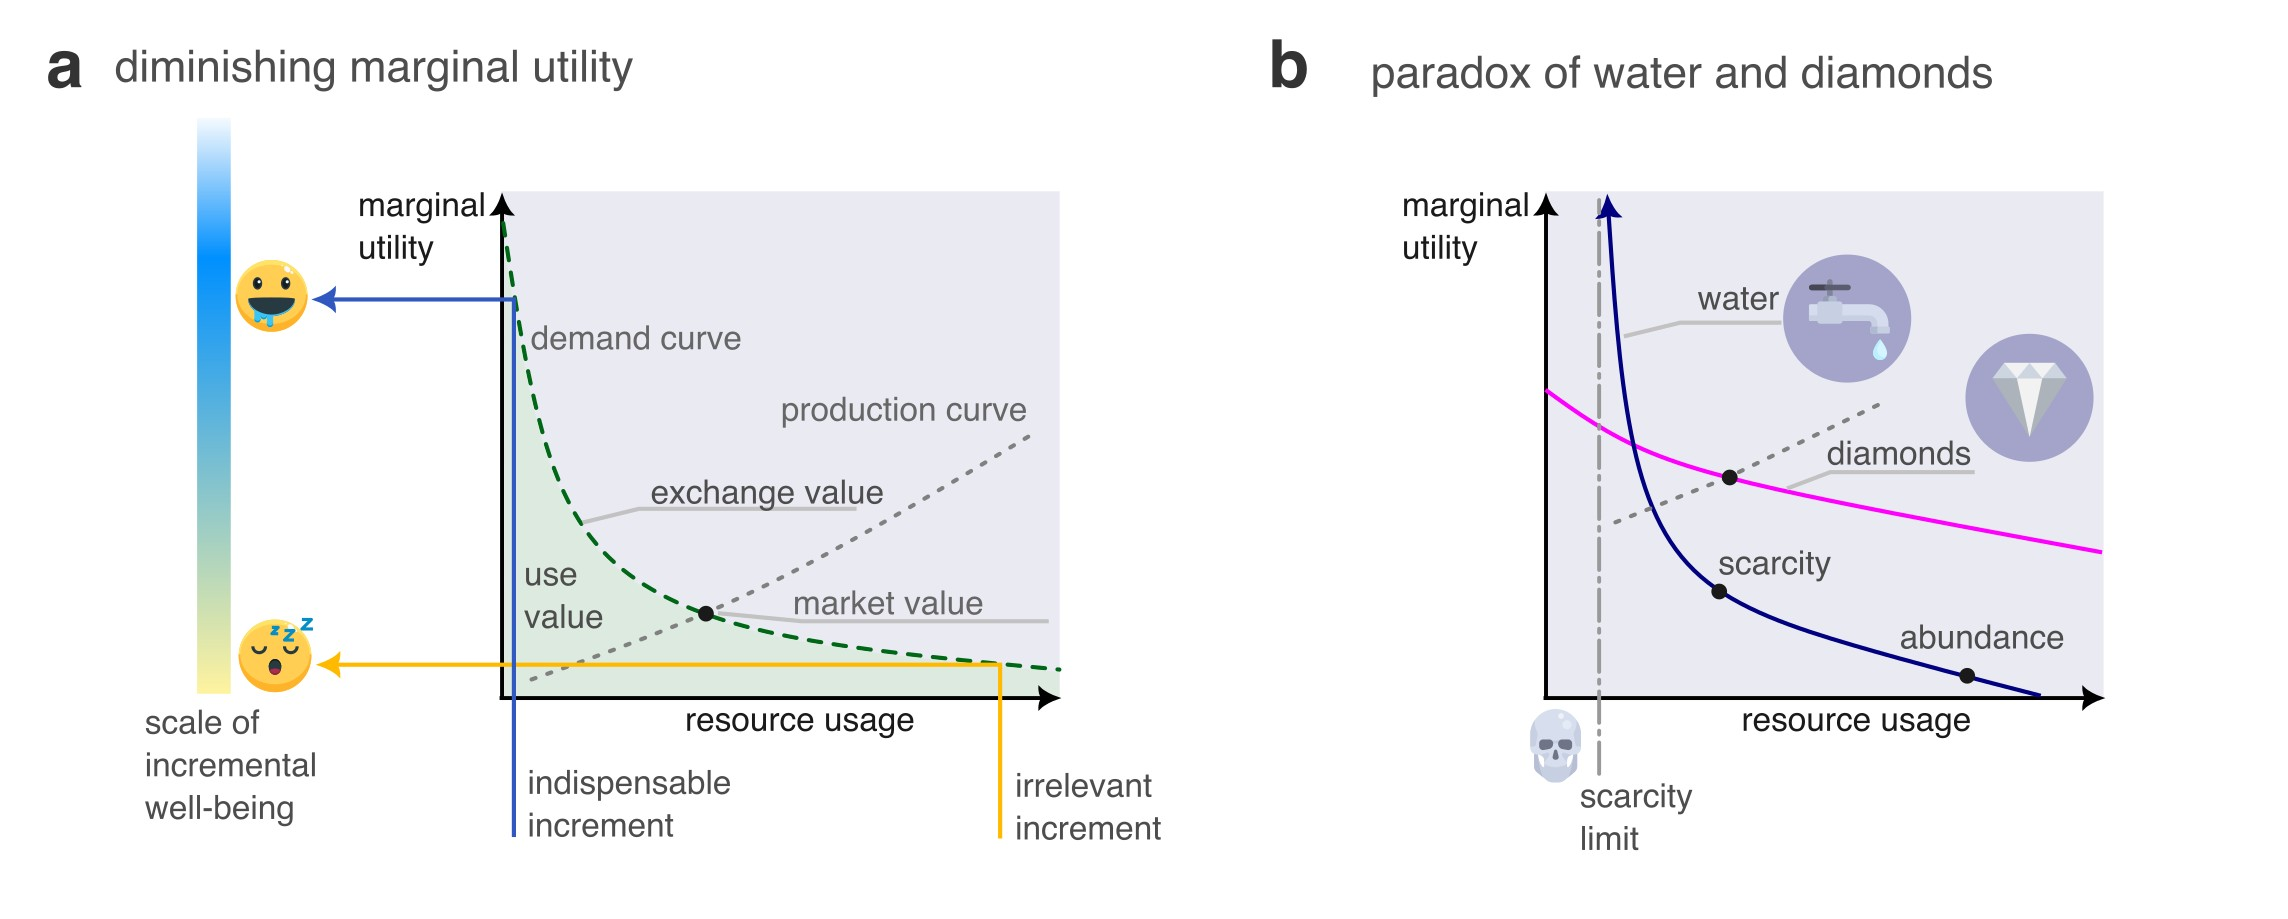
\includegraphics[width=0.98\linewidth]{figs/fig_marginalutil_en.jpg}		
\caption[Marginal Utility and Demand Curves]
{\textbf{---\;Marginal utility and demand curves.}
    The theory of marginal utility explains the observed price system in markets. Marginal utility, therefore, is equivalent to the exchange value of resources. 
    \;\textbf{a}\;---\;The theory is founded on the principle of diminishing marginal utility, the concept that the economic agent’s consumption gradually satisfies them as they consume a given resource, forming a downward-sloping demand curve. Initially, the first units consumed produce high marginal utility, an indispensable consumption increment. But marginal utility decreases as consumption increments become irrelevant. The production curve for this resource on the supply side establishes the point at which producers and consumers are equally satisfied, forming the market price.
    \;\textbf{b}\;---\;The theory of marginal utility explains exchange value in conditions of scarcity and abundance. Water, essential to life, has low marginal utility and market value when abundant, but in scarcity, its marginal utility rises, making it valuable. In contrast, diamonds, which are non-essential, maintain high market value due to their scarcity. The scarcity limit indicates the point where the marginal utility of essential resources like water reaches critical levels, raising its exchange value far above non-essential resources.
}
\label{fig:eco:marginutil} 		
\end{figure}

\par In \gls{microeon}, \gls{gutilitarism} found its peak expression in the \textbf{\gls{marutilteo}} during the 19th century, articulated by thinkers such as William Stanley Jevons and Carl Menger \cite{Gordon2002a}. This \gls{teoria} seeks to explain prices in markets, understood as the result of thousands of independent and decentralized decisions among consumers and producers. In a free-market \gls{system}, information about a resource’s scarcity is conveyed to consumers through its \textbf{\gls{gprice}}. The \gls{marutilteo} holds that the \gls{gprice} of a good or service constitutes its \textbf{market value} or \textbf{\gls{exchaval}}, in conditions that satisfy both producers and consumers (see Figure \ref{fig:eco:marginutil}\textbf{a}). This value corresponds to the additional \gls{gutility} an individual gains by consuming an extra unit of a good, which diminishes as consumption increases — the so-called \textbf{\gls{prindecmarut}}. Practically, this means that a consumer tends to become \textit{satiated} as they consume more of a given good or service, producing a downward-sloping demand curve.

\par The \gls{teoria} successfully explains the so-called \textbf{\gls{waterdiamonds}} paradox, the bizarre value difference between diamonds (of little utility) and water (of great utility) (see Figure \ref{fig:eco:marginutil}\textbf{b}). In this case, the \textbf{\gls{useval}} of a resource essential for survival, like water, can be extremely high, while its \gls{exchaval} is relatively low, especially where water is abundant. Conversely, goods such as diamonds or jewelry have low \gls{useval} but high \gls{exchaval} due to their scarcity and the high demand from those who consider them status items (though the \gls{exchaval} is low in societies that prefer feather headdresses, for example). In a situation of extreme water scarcity, on the other hand, the \gls{exchaval} of water could easily surpass that of diamonds, as it becomes a matter of life or death. This contrast illustrates how \gls{useval} and \gls{exchaval} can diverge significantly, and how marginal \gls{gutility} helps explain the market \gls{gprice} of a good or service, regardless of its functionality.\footnote{Karl Marx’s Labor Theory of Value contrasts with \gls{marutilteo} by asserting that the \textbf{\gls{workval}} of a good is determined by the socially necessary labor to produce it, rather than by the \gls{gutility} the good provides to the consumer. According to Marx, the value of a good is proportional to the amount of labor embedded in its production, including both direct labor and the labor necessary to produce the means of production. This concept underpins Marx’s analysis of labor exploitation to accumulate capital, where goods are exchanged based on the labor value, but workers receive only a fraction of this value, creating surplus value, or profit, for the owners of the means of production. Although the \gls{workval} of a good or service may exist, the problem with Marx’s thesis is that, in practice, goods produced by workers are sold in markets for the \gls{exchaval} received by consumers.} Based on this logic, the \gls{teoria} provides a \gls{model} to explain (and predict) price formation in markets, and its concept of \textbf{\gls{pareteff}} suggests that, under certain conditions, markets reach an equilibrium, allocating scarce resources optimally to satisfy everyone without improving one person’s situation at the expense of another.

\par The explanatory power of \gls{marutilteo} seems to corroborate the concept of \gls{gutility}, as consumers and producers in real markets supposedly adjust their decisions according to marginal benefits — even without ever having heard of Jeremy Bentham or diminishing marginal \gls{gutility}. Along with other auxiliary theories, \gls{marutilteo} forms the foundation of Classical \gls{microeon}, which seeks to scientifically explain the general functioning of specific markets. This set of theories assumes that agents in the economy are fully rational, capable of maximizing their individual \gls{gutility}, and that markets operate efficiently to maximize total \gls{gutility}, reaching an equilibrium automatically, without external interventions. However, for the supposed efficiency in resource allocation to be achieved, it is necessary for there to be no \textbf{\gls{marketdist}} and for ideal conditions to be present, such as the existence of many producers, full availability of information, and the absence of speculation and advertising — factors rarely observed in reality. In addition to \gls{marketdist}, the irrational behavior of human beings, as demonstrated by Daniel Kahneman \cite{kahneman2011}, challenges the idea of completely efficient markets. Consumers and producers, influenced by cognitive biases such as loss aversion and anchoring bias, often make decisions that are not entirely rational, generating inefficiencies and price distortions.

\par Evolutionary \gls{microeon} attempts to overcome these limitations by adopting a more dynamic approach, primarily including simulations with \gls{abm-models} \cite{Bourgine2006a}. In this case, agents have bounded rationality and local information, and their interactions occur over time, in explicitly defined processes. Moreover, various institutions, beyond the market, influence and sustain resource allocation. Thus, evolutionary microeconomics provides a more robust theoretical explanation for phenomena that classical microeconomics struggles to justify. The \gls{abm-models} of the evolutionary approach, naturally chaotic and computationally irreducible, make it clearer that, although they aim to make predictions, microeconomic theories generally remain limited to exploratory modeling. These models, therefore, offer a wide \gls{explan_cap} but low \gls{pred_cap}, making empirical adequacy occur in very specific cases, typically favoring some of the \gls{aux-hyp} but not the \gls{model} in its entirety.

\subsection{Macroeconomic paradigms} \label{subsec:macroeco}

\par As previously mentioned, \gls{macroeon} differs from \gls{microeon} by seeking to explain the economy as a whole, going beyond specific markets and encompassing national and global economies \cite{samuelson2009}. The classical and neoclassical doctrines of \gls{macroeon}, however, tend to be a generalization of \gls{microeon}, expanding the view to all markets, producers, and consumers in a region of interest, such as a country. The classical macroeconomic \gls{model} consists of the \textbf{\gls{circflowexval}} between producers and consumers. In practice, this corresponds to the flow of \gls{exchaval} between firms and households, which can be measured annually by the total revenue of companies and household income. Since it is a circular flow, the total value of one must be equivalent to the other.

\par The Neoclassical school revises the classical \gls{model} by introducing injections and leakages in the \gls{circflowexval} caused by private finances (individual investments and savings), public finances (tax collection and public investments), and international finances (imports and exports). The maximization of total \gls{gutility}, regarded as the \gls{ultimategoal}, can be understood as the maximization of this \gls{exchaval} flow in the circular \gls{system}. Thus, the Neoclassical school focuses solely on the \gls{exchaval} flow in markets and strategies to increase it, a concept known as \textbf{\gls{ecogrowth}}. Differences among these strategies generally involve more or less regulation or state intervention in markets to reduce unemployment and stabilize prices. Fiscal and monetary policies aim to control the leakage of taxes and individual savings in some way. The success of a strategy, however, is tested by the increase in companies' revenues or household incomes, with this growth interpreted as a sign of progress toward the \gls{ultimategoal} of maximizing total \gls{gutility}.

\par \gls{ecoeco}, primarily articulated by Herman Daly, proposes a new \gls{paradigma} that rejects the Neoclassical school \cite{daly2011}. This perspective proposes that macroeconomic \gls{teoria} be incorporated into \textbf{\gls{ecology}}, a science based on physical principles, recognizing that the \gls{sys-target} to be modeled is, essentially, a material \gls{system} \cite{Daly1968a}. Evidently, the material perspective on \gls{gseconomics} was present in its modern origins but was slowly replaced by an interest in \gls{exchaval}, which is immaterial \cite{Christensen1987}. A good example is that of Thomas Malthus (1766-1834), who identified potential limits to human population growth based on food production, which would grow at a relatively slower pace. In essence, Malthus clearly saw humans as material beings who need nutrients and energy to survive, like any other species on the planet. For example, if a human needs to consume 3 liters of water and 0.4 kg of food daily (approximately 2000 calories, divided among fats, carbohydrates, and proteins), it follows that today’s global population of 8 billion people demands 24 million cubic meters of water and 50,000 tons of food daily. Without a material flow of this magnitude, the global population would not survive for long. Eight billion seems like a large number, but would it be possible to double or triple that number?

\par Since Malthus's predictions of widespread famine and population collapse did not materialize in his time, classical and neoclassical economists tend to dismiss his \gls{teoria}, confusing his circumstantial conclusions with the material foundations of his approach. In the heated debate that arose with the proposal of \gls{ecoeco}, neoclassical economists accuse proponents of the new \gls{paradigma} of being \say{neo-Malthusians}, a term with a somewhat pejorative connotation \cite{Forrester1974}. The ecological perspective, in turn, accuses the Neoclassical school of being excessively focused on the \gls{exchaval} flows of \textbf{\gls{marktegoods}}, very specific goods and services that can be bought or sold \cite{Daly1997a, Daly1997b}. This focus on value flow is so dominant that the Neoclassical school does not even consider the materiality of \gls{marktegoods}; they are merely \textit{vehicles} that carry marginal \gls{gutility}, defined by their \gls{gprice}. Thus, the Neoclassical school instantiates an immaterial and abstract ontology of \gls{exchaval}. This representation may be an interesting \gls{model} for understanding and explaining value flows in markets, but it is far from being a representation of material reality.

\subsection{The ontology of physicalism} \label{subsec:physicalism}

\par Ontologically, \gls{ecoeco} upholds a physicalist reality. \textbf{\gls{gphysicalism}}\footnote{Also known as Materialism.} is a realist and naturalist line of thought that posits that objective reality exists, is governed by the laws of Physics, and ultimately comprises matter and energy \cite{sep-physicalism}. As Physics is a scientific \gls{teoria}, \gls{gphysicalism} forms the primary worldview directly implied by Scientific Realism. From this perspective, even the concept of \gls{gutility} is considered material, as notions like \say{well-being} or \say{satisfaction} are, in reality, synapses in brains, an organ of the human body.

\par Despite its appeal due to strong empirical adequacy, \gls{gphysicalism} faces some critical structural problems. One major issue is the mind-body problem, or the \textbf{\gls{consproblem}} — the apparent impossibility of explaining subjective experiences from physical processes like synapses \cite{sep-consciousness}. Another serious issue is the \textbf{\gls{willproblem}}, which arises when accepting the ultimate consequences of \gls{gphysicalism}, namely Determinism \cite{sep-skepticism}. In a deterministic reality, decisions would merely be sensations, devoid of real agency, rendering the idea of choices in resource allocation, central to \gls{gseconomics}, meaningless\footnote{Radical \gls{gphysicalism} leads to Nihilism, an ethical \gls{teoria} that denies the existence of moral values or ultimate objectives to guide decisions}. However, both issues are symptomatic of Scientific Realism, which proposes that Science aims to describe the truth about reality. Instrumentalists, such as Bas van Fraassen and Nancy Cartwright, contest this view, arguing that scientific theories aim merely to produce \textit{empirically adequate} descriptions without necessarily reflecting the ultimate truth about the world \cite{bas1980, nancy1983}. In this sense, choosing a physicalist ontology for \gls{macroeon} provides a more empirically robust foundation than the Neoclassical school, whose explanation is limited to the flow of \gls{exchaval} in markets. Whether true or not, a physical basis offers greater \gls{explan_cap} and predictive capability than the Neoclassical circular flow \gls{model}.

\par One of the pioneers in accepting and promoting \gls{gphysicalism} within \gls{gseconomics}, laying the groundwork for the ecological \gls{paradigma}, was Nicholas Georgescu-Roegen (1906-1994), especially with his seminal work \textit{The Entropy Law and the Economic Process} (1971). In this work, Georgescu-Roegen emphasizes the implications of the first and second laws of thermodynamics for an economy based on material resources. The \textbf{\gls{firstlaw}}, known as the \textbf{principle of conservation}, states that matter and energy can neither be created nor destroyed, only transformed from one form to another. The \textbf{\gls{secondlaw}}, on the other hand, establishes that the \textbf{entropy} of an isolated \gls{system} tends to increase, indicating that natural processes follow a trajectory of increasing disorder. This means that \textbf{free energy}, capable of performing work, tends to degrade into forms less capable of doing work. Similarly, material structures tend to spontaneously disintegrate from an ordered (heterogeneous and less probable) state to a disordered (homogeneous and more probable) state. The second law also implies that no process of energy transfer or material conversion is 100\% efficient, as there will always be losses in the form of heat and waste. Therefore, these laws establish that the maintenance of order in the Universe is only possible locally and at the cost of external sources of free energy. Even so, the creation of order through work inevitably results in the generation of material and energetic waste without \gls{gutility}.

\par Another pioneer of the physicalist view was Jay Forrester, the inventor of \gls{sys-dyn}, a topic introduced in Chapter \ref{chap:systems}. Jay Forrester and his team of engineers and scientists at \texttt{MIT} demonstrated through the publications \textit{World Dynamics} and \textit{Limits to Growth} how compartmental models can be employed to obtain predictions about the state of the global economy over time \cite{Forrester1973a, meadows1974}. The simulations of the \texttt{World3} \gls{model} introduced a physicalist approach, demonstrating the materiality of the economic \gls{system} by integrating the levels and material flows of the global \gls{system}, such as population, industrial capital, arable land, and resulting pollution. The results, although varied across different scenarios, highlight the physical limits imposed by the \gls{biosf} on the \gls{antroposf}, such as the depletion of non-renewable energy sources, agricultural land degradation, and the finite capacity of ecosystems to absorb pollutants. In the various scenarios explored, human population growth and industrial capital inevitably encounter a tipping point, where increasing resource extraction costs, agricultural productivity loss, and pollution impacts impose increasingly negative feedbacks, eventually leading to a decline in industrial capital growth. Thus, the explorations of \texttt{World3} illustrated the interdependence between the economic \gls{system} and the physical limits of the \gls{biosf}.

\subsection{The ecological model of macroeconomics} \label{subsec:ecomodel}

\begin{figure}[t!] 
\centering				
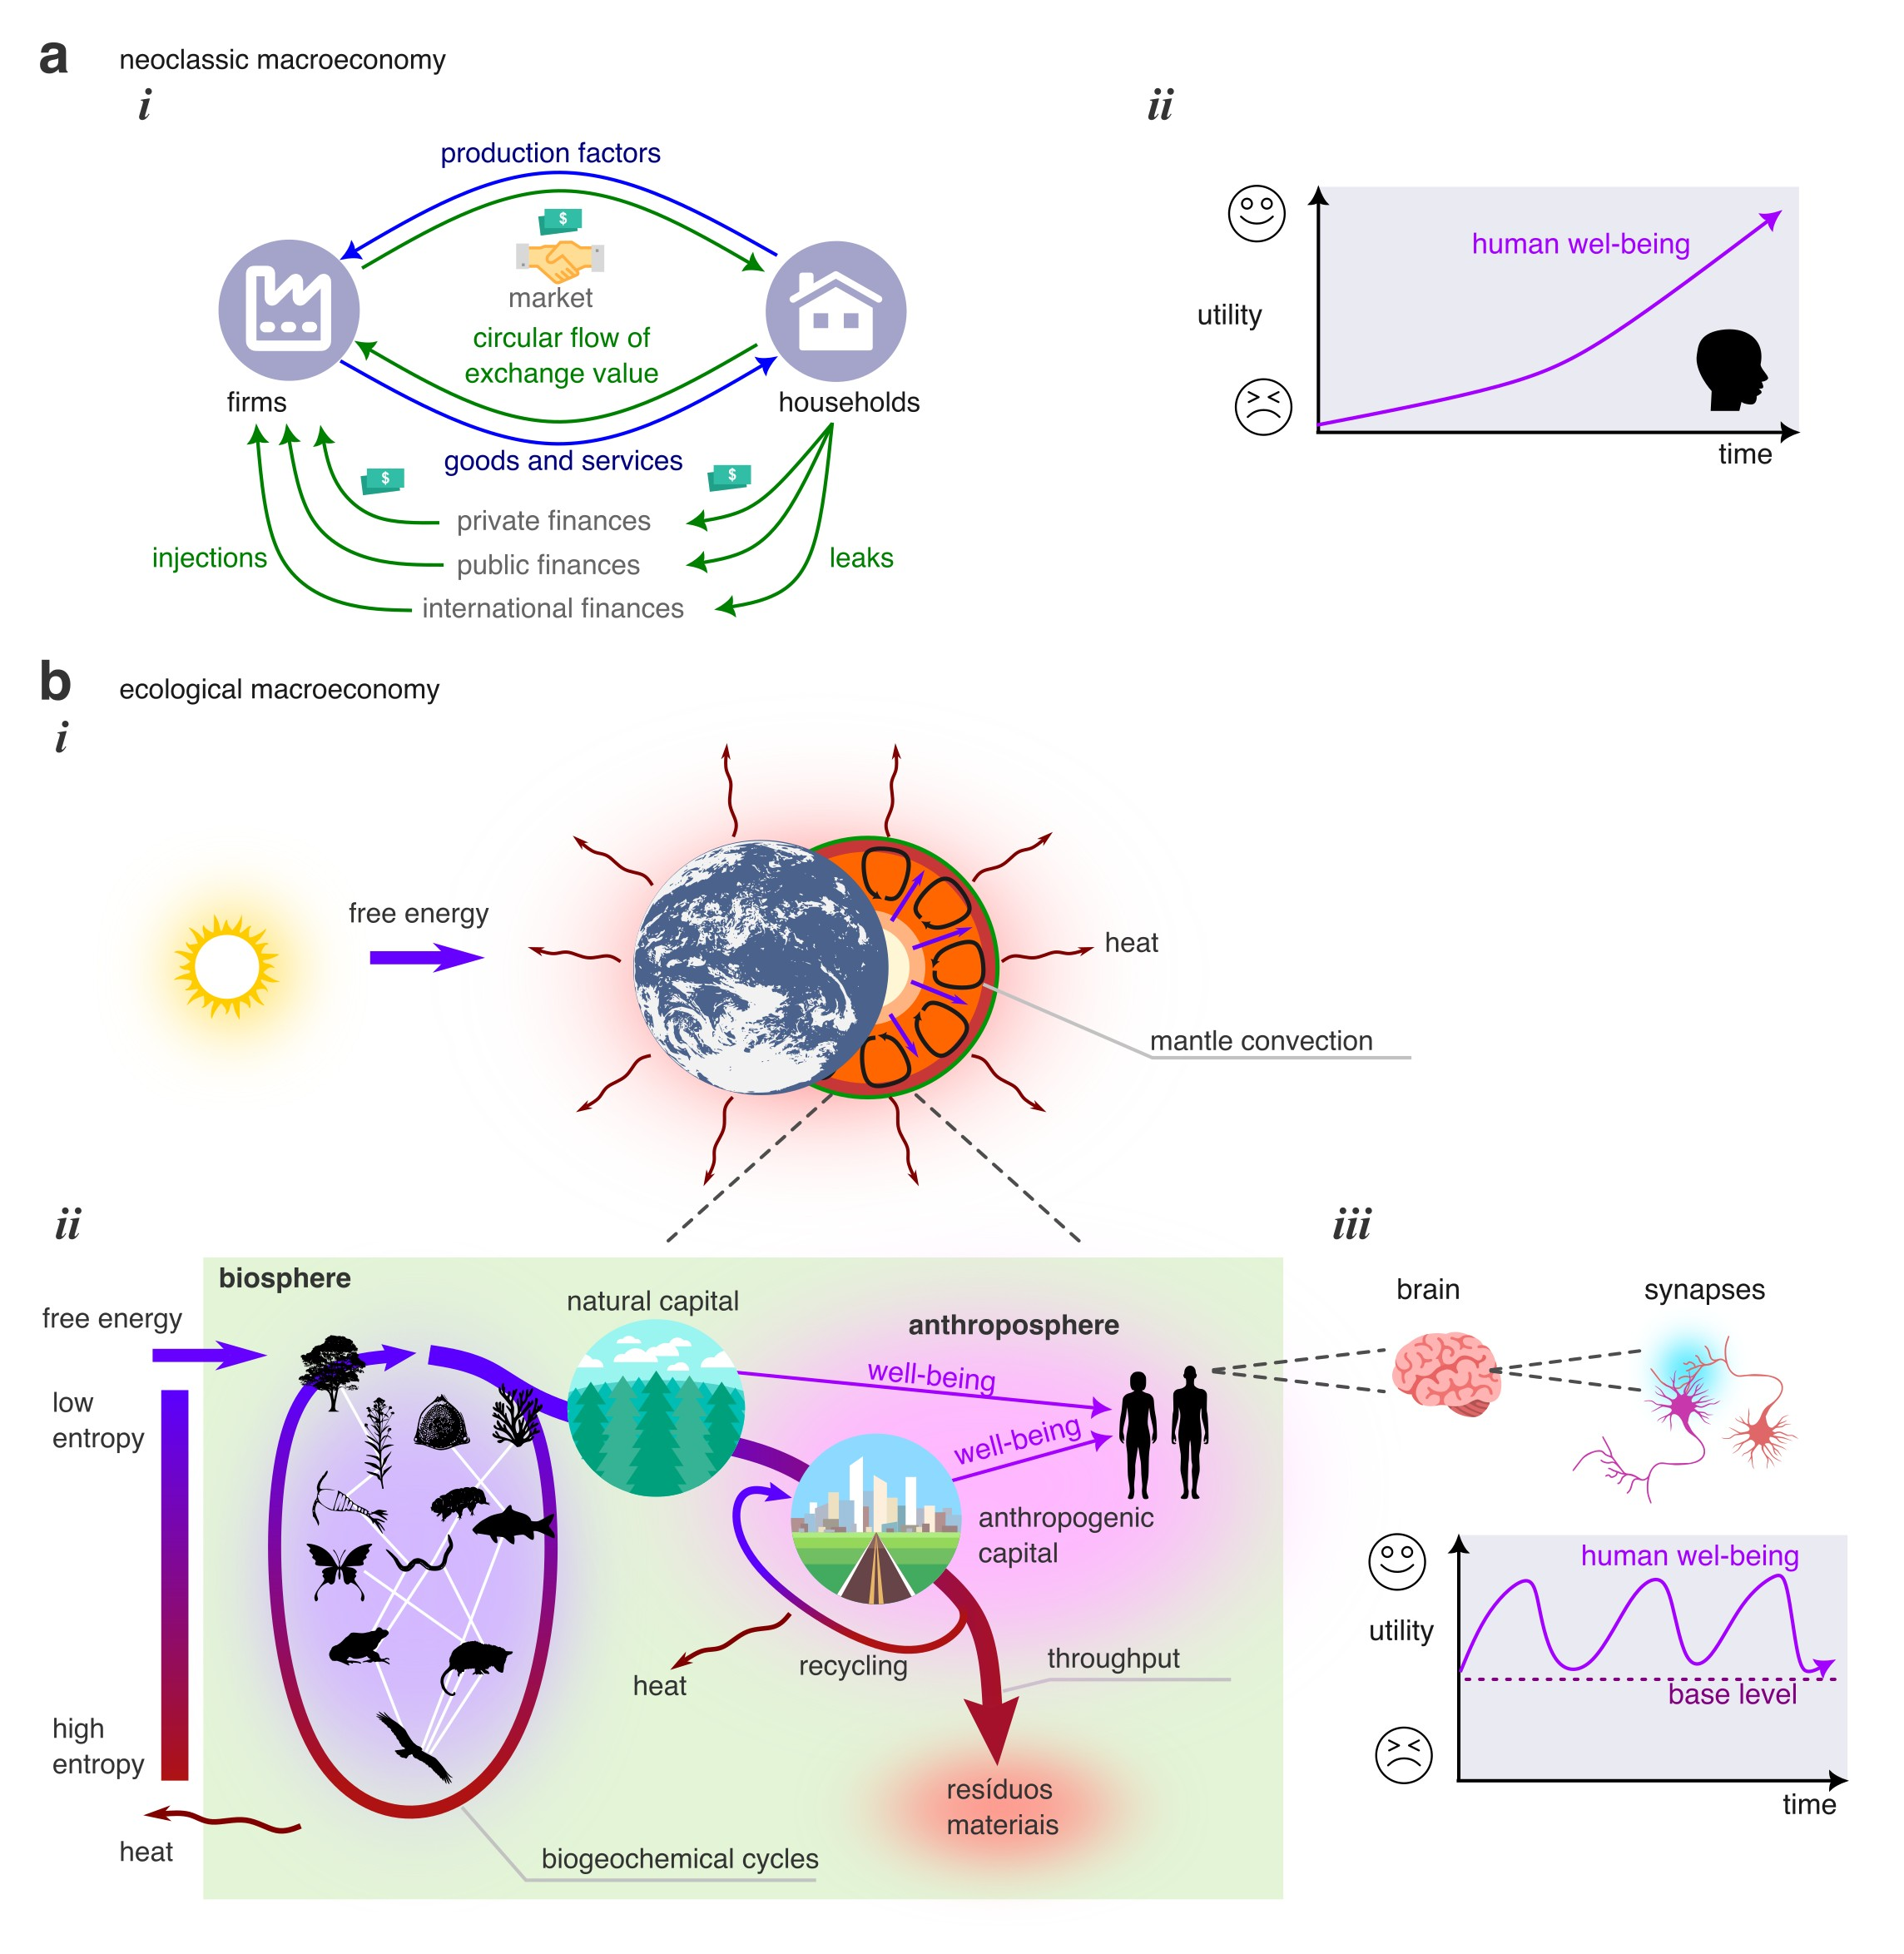
\includegraphics[width=0.98\linewidth]{figs/fig_ecomodel_en.jpg}		
\caption[Ecological \gls{macroeon}]
{\textbf{---\;Ecological \gls{macroeon}.}
    Unlike neoclassical macroeconomics, ecological macroeconomics instantiates a model based on the laws of thermodynamics.     
    \;\textbf{a}\;---\;The neoclassical macroeconomic model seeks to represent a circular flow of exchange value between firms and households, with injections and leakages generated by fiscal and financial policies of private and public agents (detail \textrm{\textit{i}}). If the exchange value flow increases, utility increases, as exchange value is equivalent to marginal utility. Consequently, it is concluded that an increase in the exchange value flow is a direct indicator of increased human well-being (detail \textrm{\textit{ii}}).    
    \;\textbf{b}\;---\;The ecological macroeconomic model assumes a physicalist ontology, instantiating matter and energy flows in open systems. The biosphere is the Earth’s upper layer that slowly exchanges matter with the mantle and receives free energy flows from the Sun and core, emitting heat to space (detail \textrm{\textit{i}}). The free energy flow in the biosphere is processed by biogeochemical cycles, including ecosystems, circulating materials between high and low entropy states. The anthroposphere consists of the human habitat embedded within the biosphere and is traversed by a linear flow of matter, resulting in waste (detail \textrm{\textit{ii}}). In this system, human well-being is also a material and finite process, derived both from anthropogenic capital, the structures of the anthroposphere, and directly from natural capital, the pre-existing structures in the biosphere (detail \textrm{\textit{iii}}).
}
\label{fig:eco:ecomodel} 		
\end{figure}

\par Based on thermodynamic laws and a systemic view, \gls{ecoeco} represents macroeconomics through an ecological \gls{model}, illustrated in Figure \ref{fig:eco:ecomodel}. In this \gls{model}, the \textbf{\gls{antroposf}} – the material environment inhabited by humans – is embedded within the \textbf{\gls{biosf}}, encompassing Earth’s material \gls{system}, from the atmosphere to the first kilometers of the lithosphere. Energetically, the \gls{biosf} is not an isolated \gls{system} but an open one, receiving a continuous flux of free energy from solar radiation and Earth’s inner core. This high-quality energy, after performing work, is emitted into space as less useful forms of heat. Materially, the \gls{biosf} is also connected to input and output flows driven by subduction, burial, uplift, and volcanism processes, which result from mantle convection, along with the loss of light gases into space. Although processes like volcanism are more abrupt exceptions, most material exchanges in the \gls{biosf} occur extremely slowly on geological scales. Thus, the \gls{biosf} can practically be considered an energetically open but materially closed \gls{system}.

\par The energy openness of a \gls{system} is essential for creating order within it. Photosynthesis, for example, is one of the main order-generating processes in the \gls{biosf}, employing free energy from solar radiation to produce low-entropy materials, such as sugars, from high-entropy compounds like carbon dioxide. The burial of these low-entropy materials over millions of years produced the fossil fuel reserves widely used today by the \gls{antroposf}. Beyond photosynthesis, the driving force behind the carbon cycle, various other \textbf{biogeochemical cycles} occur in the \gls{biosf}, all powered by external energy sources. The \gls{hydro_cicle}, for instance, is driven by solar energy, which evaporates water and raises it, imparting gravitational potential that can perform work in mills or turbines. These cycles maintain the dynamics and order of the \gls{biosf}, demonstrating the interdependence between external energy input and internal system organization.

\par The physical foundations of \gls{ecoeco} result in a completely different interpretation of \gls{ecogrowth}. The \gls{firstlaw}, viewed through the lens of the ecological \gls{model}, implies that no real material growth exists in the \gls{biosf}, as matter is conserved. The \gls{antroposf}, as a human habitat within the \gls{biosf}, can expand its structural complexity by processing materials from the \gls{biosf}, but always at the cost of generating heat and other waste. The \gls{secondlaw}, in turn, implies that merely \textit{sustaining} the anthroposphere requires a flow of free energy and replacement materials, as it is necessary to continuously work against the spontaneous degradation of the material \gls{system}. This inevitable flow of matter processed by the \gls{antroposf} and generating useless waste dispersed into the \gls{biosf} is called \textbf{\gls{gthoughput}} in \gls{ecoeco}\footnote{Free translation of \textit{throughput}.}. In this sense, the \gls{ecogrowth} theorized by Neoclassical \gls{gseconomics} is, above all, an illusion, an imaginary phenomenon instantiated by the intersubjective reality of \gls{exchaval}. However, since goods and services in markets are material entities, increasing their consumption necessarily implies increasing \gls{gthoughput}. The difference between economic paradigms becomes very clear here: while one instantiates a circular and immaterial flow (marginal \gls{gutility} and exchange value), the other envisions a linear and material flow (processing of free energy).

\section{Natural capital} \label{chap:ecoeco:natcap}

\subsection{The optimal scale of the anthroposphere} \label{subsec:escaleopt}

\begin{figure}[t!] 
\centering				
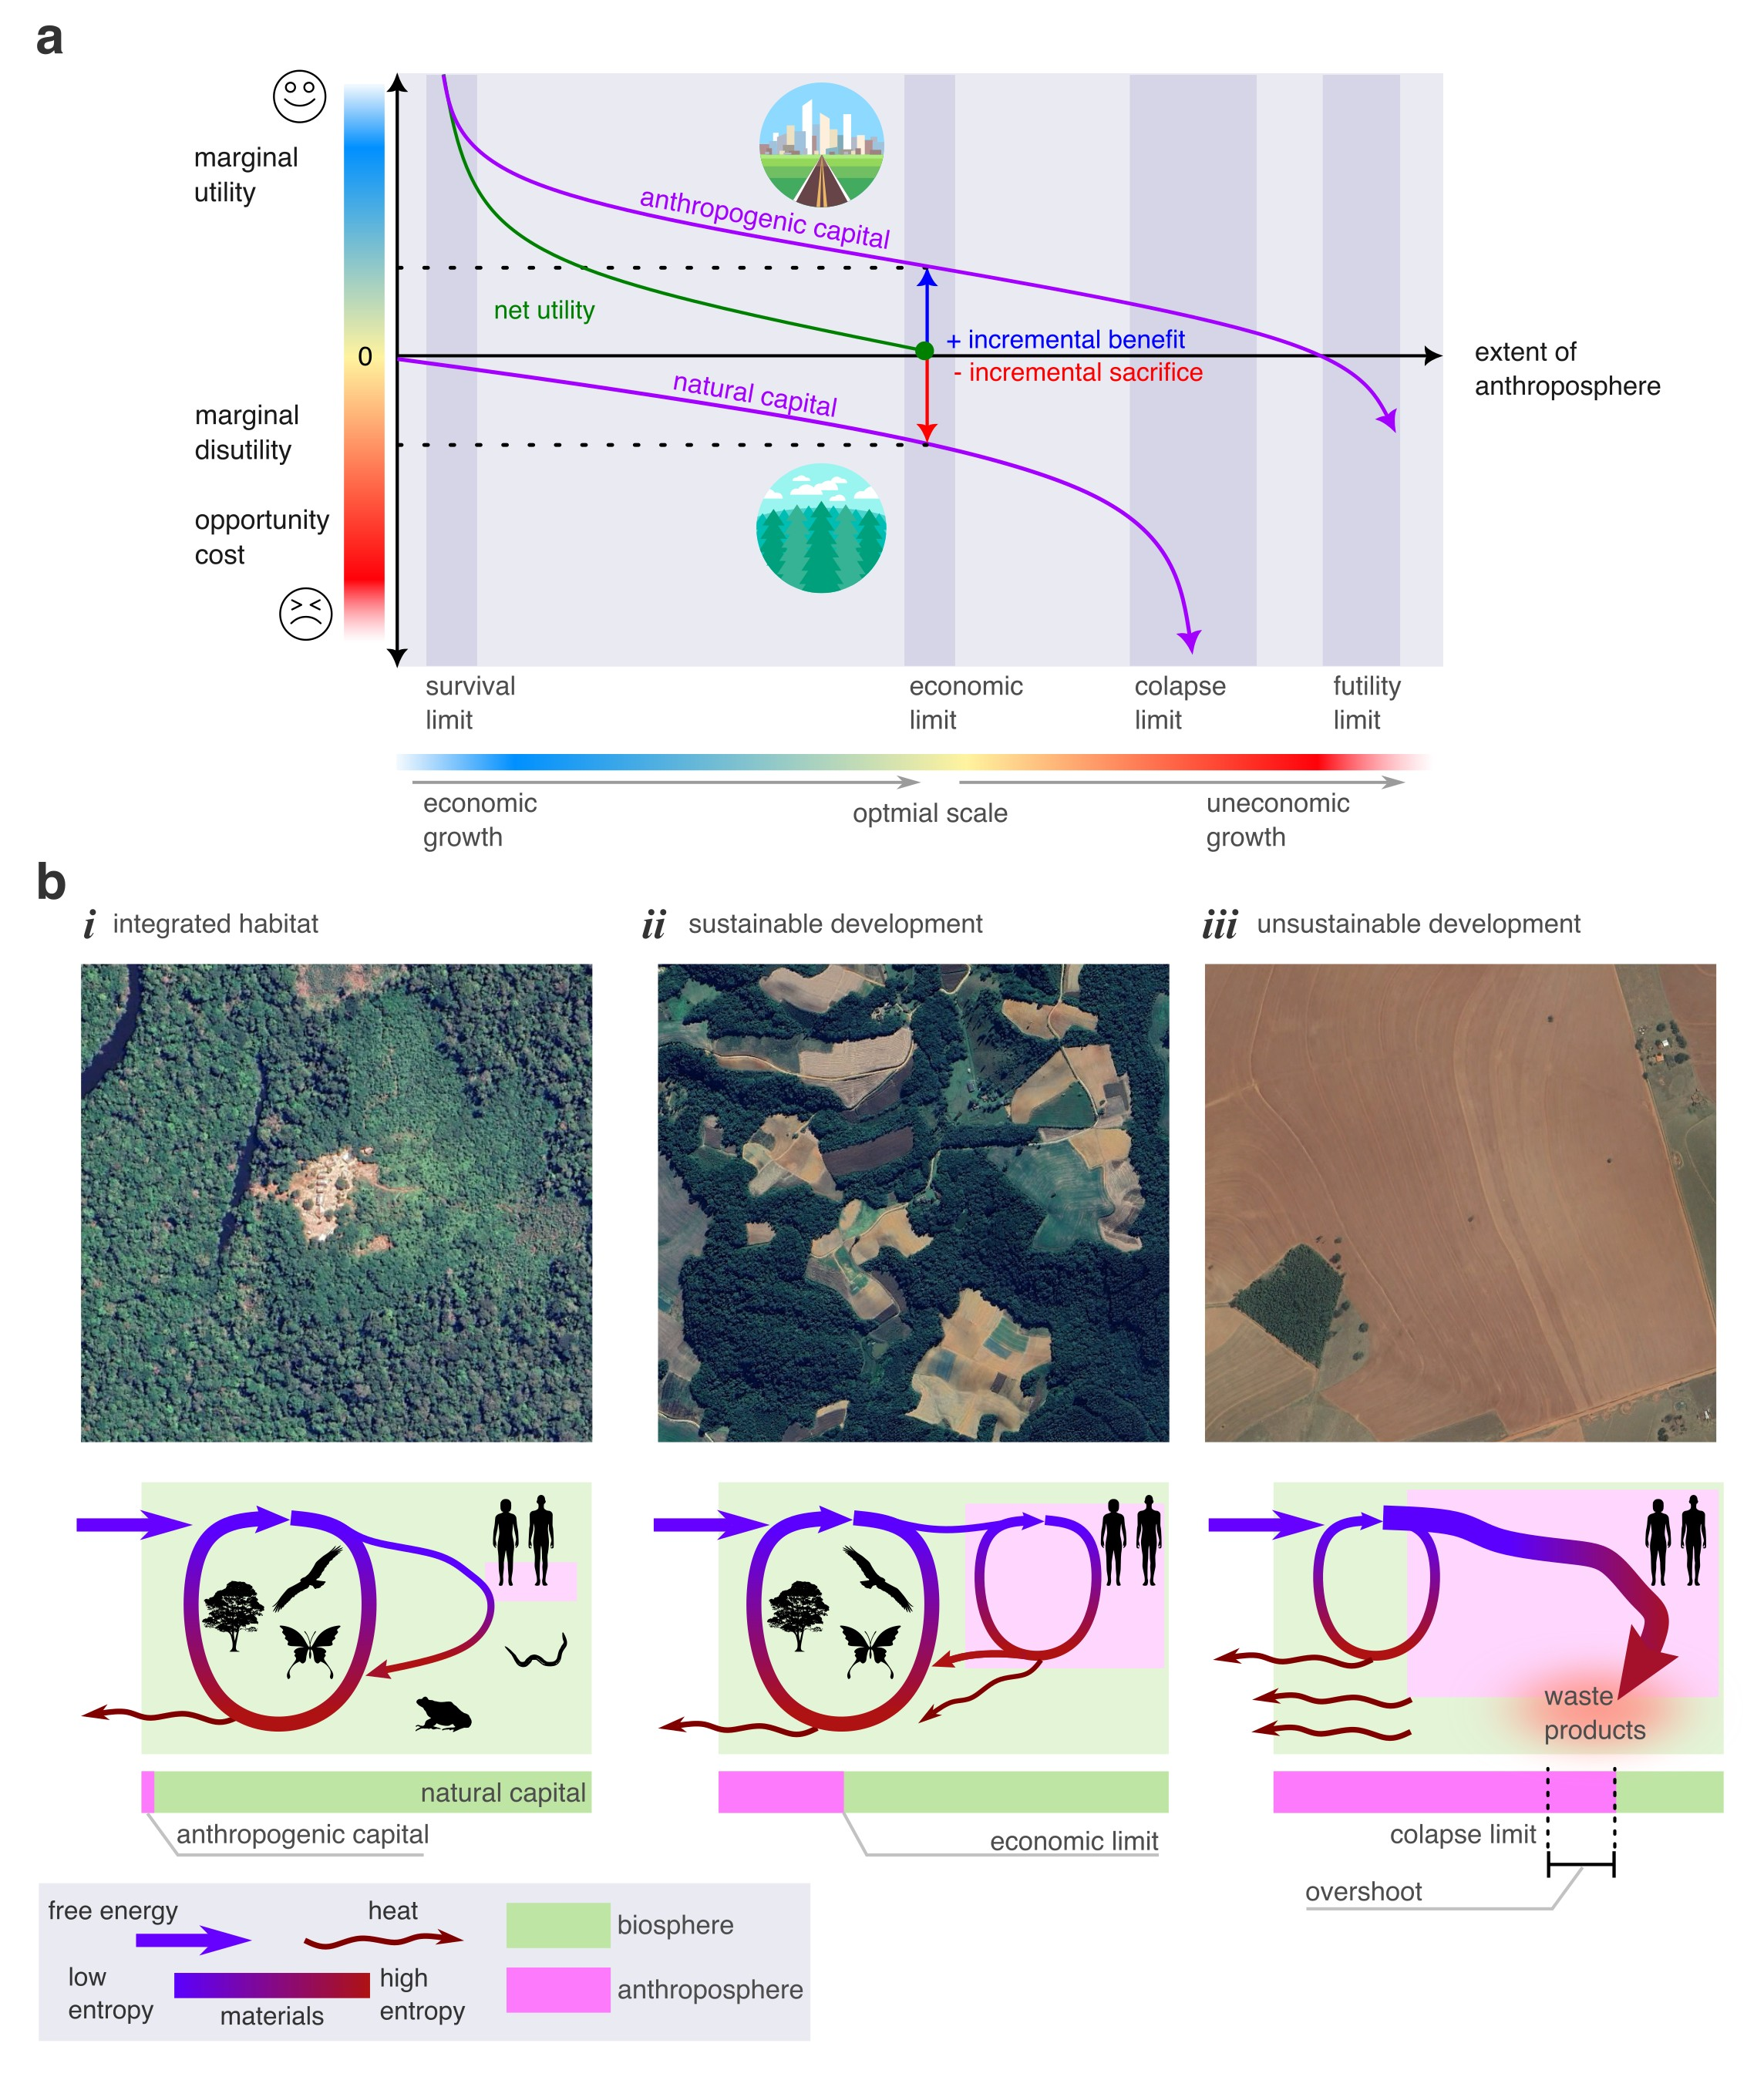
\includegraphics[width=0.98\linewidth]{figs/fig_optscale_en.jpg}		
\caption[The Optimal Scale of the Anthroposphere]
{\textbf{---\;The optimal scale of the anthroposphere.}
    The main implication of the ecological macroeconomic model is that, being material, the anthroposphere imposes an economic extension over the biosphere, or an optimal scale. The research questions of the ecological paradigm revolve around identifying the optimal scale and other limits from different perspectives.
    \;\textbf{a}\;---\;The expansion of the anthroposphere incurs both diminishing marginal utility and an opportunity cost, or marginal disutility, due to the sacrifice of natural capital for the expansion of anthropogenic capital. The survival limit, therefore, is the minimally viable habitat that humans need to metabolize and reproduce. The economic limit is the scale at which the incremental benefit is equivalent to the incremental sacrifice. Beyond the optimal scale, the expansion of the anthroposphere is anti-economic, as it results in negative net marginal utility. In this region, there is the collapse limit, which varies according to the scale of analysis, and the futility limit.
    \;\textbf{b}\;---\;The optimal scale can be visualized by land use, showing the gradual transition from integrated habitat with small open clearings (detail \textrm{\textit{i}}), through a mosaic of fragmented areas (detail \textrm{\textit{ii}}), to complete anthropization (detail \textrm{\textit{iii}}). Sustainable development represents the maximum size of the anthroposphere that can still be integrated into the ecological system, which requires a resource recycling flow.
}
\label{fig:eco:escaleopt} 		
\end{figure}

\par Although \gls{ecoeco} rejects neoclassical ideas in \gls{macroeon}, it shares several fundamental concepts of \gls{microeon}, such as \gls{marutilteo} and the \gls{ultimategoal} of maximizing \gls{welbeing}. In this sense, Herman Daly \cite{Daly2015a} proposes that, as the \gls{antroposf} is a material sub\gls{system} of the \gls{biosf}, there exists an \textbf{optimal scale} for the \gls{antroposf}, the point at which \gls{welbeing} reaches its maximum, as illustrated in Figure \ref{fig:eco:escaleopt}. Beyond the so-called \textbf{\gls{ecolimit}}, the growth of the \gls{antroposf} becomes anti-economic, generating increasing detriments. The concept of \textbf{\gls{sustdev}} is directly tied to this idea, indicating that the material growth of the economy must be balanced within the limits of the \gls{biosf}. Thus, economic choices need to consider this balance, implementing mechanisms and policies that prevent the \gls{antroposf} from exceeding its optimal point. The research agenda of this \gls{paradigma} therefore aims to investigate how close we are to this limit. In an empty world, there is room to expand. In a crowded world, however, this limit may have been surpassed, requiring planning that prioritizes the \textbf{degrowth} of the \gls{antroposf}.

\par Understanding the optimal scale is only possible by generalizing the concept of \textit{capital} beyond its conventional conception. In the ecological view, \textbf{\gls{antcap}} consists of the material and social structures built by humans that produce a flow of goods and services, resulting in \gls{welbeing}. The definition is vague and may be confused with the \gls{antroposf} itself. A motorcycle factory, for example, is a typical example of industrial capital that produces goods (motorcycles). However, a motorcycle can be used to provide a delivery service, making it a good on one hand and capital on the other. The ability to ride a motorcycle makes the workers of a delivery company its human capital. The term \say{capitalism}, in this sense, consists of the doctrine of accumulating \gls{antcap} or expanding the \gls{antroposf}. It should be noted that, from the neoclassical perspective, capitalism explicitly dictates capital growth but only indirectly assumes that this will increase human well-being by increasing the flow of \gls{exchaval}. As we have seen, this doctrine results in the expansion of the \gls{antroposf} over the \gls{biosf}, increasing \gls{gthoughput}.

\par Beyond \gls{antcap}, the ecological view also introduces the concept of \textbf{\gls{natcap}}. The idea was initially articulated by Robert Costanza and Herman Daly, in \gls{analogy} to built capital \cite{Costanza1992a}. Thus, \gls{natcap} is defined by the material structures of the \gls{biosf} itself that produce a \textit{direct} flow of goods and services, resulting in \gls{welbeing}. In addition to directly usable goods, such as timber or fish stocks, services like pollination, which supports food production, fertile soil formation, essential for agriculture, and biogeochemical cycles like carbon sequestration, which regulates the global climate, are also considered. These services stem from fundamental \textbf{environmental functions} essential to life on Earth, even though they are often overlooked by the conventional approach to \gls{natrec} \cite{Groot1987a}. A good exercise to illustrate their importance is to imagine what would be required to reproduce natural conditions in a human colony on Mars. Without the support of \gls{natcap}, all processes essential to life would need to be artificially replicated, highlighting the critical interdependence between the \gls{antroposf} and the \gls{biosf}.

\par The core of the optimal scale concept, therefore, is to recognize that constructing \gls{antcap} requires dismantling the existing \gls{natcap} infrastructure. This necessarily results in a sacrifice of well-being provided directly by resources and \gls{natserv}. In economic jargon, there is an \textbf{\gls{opcost}} to the expansion of the \gls{antroposf}, which is the sacrifice of resources and \gls{natserv} provided by \gls{natcap}. \gls{marutilteo} helps illustrate this dilemma through the \gls{gutility} diagram (Figure \ref{fig:eco:escaleopt}): the \gls{ecolimit} of \gls{antcap} growth occurs when its marginal \gls{gutility} equals its \textbf{\gls{desutilmar}}. \gls{desutilmar} consists of the incremental loss of \gls{gutility} on the \gls{natcap} side and is exactly the \gls{opcost}. This incremental sacrifice of \gls{gutility} is small in an empty world: a small clearing in an immense forest is practically imperceptible in terms of detriments, even at the \gls{loc-scale} of the ecosystem. Indeed, it can be conceived that the \gls{antroposf} requires a minimally viable limit, the \textbf{survival limit} of humans in the \gls{biosf}. But as the world becomes crowded, the losses in \gls{gutility} grow non-linearly. In many cases, it is possible for a \textbf{\gls{colaplimit}} to be exceeded, when virtually irreversible degradation processes are triggered. The overload region is a dangerous situation, as crossing the collapse limit does not imply an immediate catastrophe due to the delay in the propagation of impacts within the ecological system. The diagram represents the entirety of the \gls{biosf} but can also be interpreted at other scales, such as countries, watersheds, etc., and in relation to specific natural processes. In a watershed, for example, the \gls{ecolimit} would be a balanced land occupation and water use that preserves various other goods and \gls{natserv}. A more intuitive example is the global climate \gls{system}: the \gls{ecolimit} would be a greenhouse gas pollution level balanced in terms of well-being, while the \gls{colaplimit} represents a pollution level at which climate change processes become uncontrolled, triggering positive feedback loops.

\par The \gls{ecolimit} and \gls{colaplimit} are generally lower than the \textbf{\gls{futilelimit}}, the level at which the marginal \gls{gutility} of \gls{antcap} is zero or even negative (the situation when more resources directly bring \textit{less} well-being). This brings important political implications that challenge the social \textit{status quo}. The Neoclassical economic school tends to be well-regarded by social elites, as it suggests that simply increasing resource consumption will raise collective well-being, regardless of the relative inequalities among consumers. With the so-called \textbf{promise of a bigger slice}, it is enough to make the \say{pie} grow for everyone so that the poorer will have a larger slice tomorrow than today — even if the slicing remains unfair. But by admitting that an optimal scale exists for the \gls{antroposf}, we see that resources should be consumed at the \gls{ecolimit} to maximize \gls{welbeing}, far below the \gls{futilelimit}. The only viable way for someone to consume resources above the \gls{ecolimit} is to ensure that others consume far below, one compensating for the loss of \gls{natcap} by the other. Since this unequal arrangement does not maximize collective well-being, \gls{ecoeco} postulates that, in a finite material world, inequality is immoral.

\subsection{Understanding natural resources} \label{subsec:natrec}

\begin{figure}[t!] 
\centering				
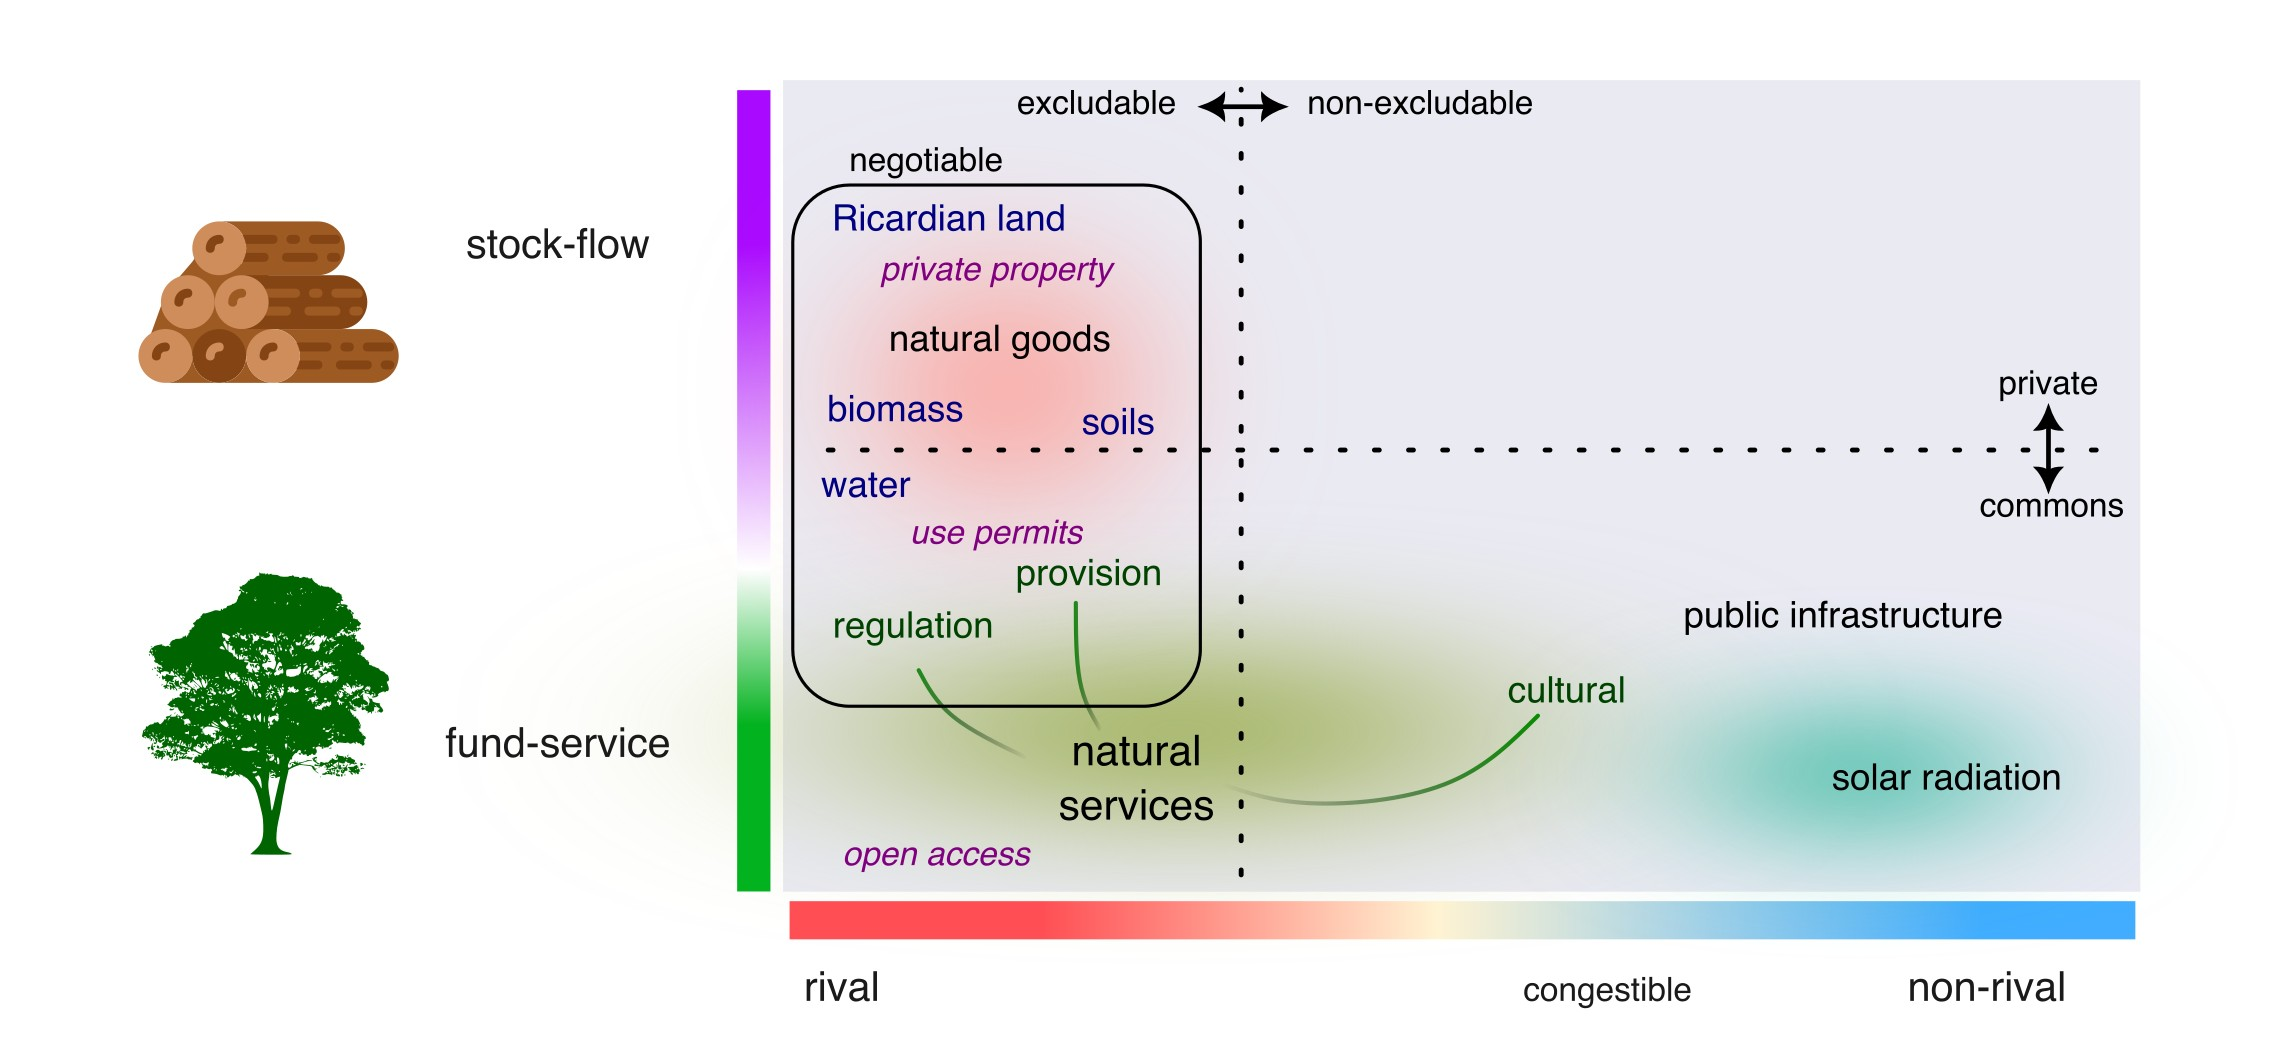
\includegraphics[width=0.98\linewidth]{figs/fig_natrec_en.jpg}		
\caption[Classification of Natural Resources]
{\textbf{---\;Classification of \gls{natrec}.}
    The ecological paradigm organizes scarce resources into stock-flow and fund-service typologies. Stock-flow resources provide utility when materially transformed during their consumption, while fund-service resources provide utility without being transformed. Stock-flow resources can be consumed at any rate but are depleted suddenly. Fund-service resources can only be consumed at a maximum possible rate and can eventually become congested. All stock-flow resources are rivals by definition, meaning multiple users cannot consume them simultaneously, and all non-rival resources, by definition, are fund-services. Natural services, unlike raw materials, are generally rival fund-services and therefore require some regulated form of exclusivity to avoid the tragedy of the commons.
}
\label{fig:eco:natrec} 		
\end{figure}

\par The classification of \textbf{\gls{natrec}} by \gls{ecoeco} contrasts sharply with the approach of the Neoclassical school. Since Neoclassical \gls{macroeon} tends to be an extended view of \gls{microeon}, this \gls{paradigma} treats resources homogeneously, reducing them to mere inputs, or \textbf{factors of production}, that contribute to maximizing goods and services through \gls{antcap}. In general, these factors are categorized as \say{land} (raw materials) and \say{labor} (workforce), along with capital itself (machinery and equipment). In the Neoclassical view, the idea of \textbf{substitutability} prevails, implying the possibility of substituting one input for another when it becomes scarce, which creates a relative insensitivity to resource depletion. By not recognizing \gls{natcap}, resource depletion is not seen as a fundamental problem, provided that technological innovations allow for substitutions.

\par Nonetheless, Herman Daly articulates a critical distinction between \textbf{\gls{recstflow}}, which can be consumed at any rate, and \textbf{\gls{fundserv}}, whose productivity is time-limited and cannot be easily substituted \cite{daly2011}. \gls{natcap} can be of either type — or both, as in the case of forests. Forests are a stock-flow of timber, a raw material. But they are also a fund-service of various \textbf{\gls{natserv}} (see Figure \ref{fig:eco:natrec}). Here, the \gls{scale_problem} becomes evident: the \gls{econbenefit} of dismantling a forest comes with the \gls{opcost} of the sacrificed \gls{natserv}. However, since forests are a \gls{system} that regenerates with solar energy, it is possible to find a sustainable flow of timber extraction without entirely giving up \gls{natserv}. This classification highlights the need for strategies that consider the limits and \textbf{irreplaceability} of certain resources, providing a more suitable framework for designing \gls{sustdev} policies.

\par \gls{recstflow} are those resources materially transformed during the production process, meaning they become part of the final product. In the context of \gls{natcap}, these resources are classified as \textbf{\gls{recrenew}} and \textbf{\gls{recnotrenew}}. A clear example is oil, which is refined into fuel, or trees, which are converted into boards and paper. When available, these resources can be consumed at nearly any rate. For instance, large quantities of oil can be quickly extracted if enough wells and refineries are in operation. Similarly, a forest can be cleared within days if sufficient machinery and workers are available. These resources can also be stored for future use; raw materials like grains, fuels, and minerals can be stockpiled, allowing for flexible management over time. Similarly, forest stands can be preserved for future harvesting.

\par When consumed at a rate exceeding the \textbf{\gls{carycap}}, \gls{recstflow} resources become suddenly depleted. Since oil takes millions of years to form naturally, it is considered a non-renewable resource, as is the case with most \textbf{\gls{recmineral}}. Forests, however, when properly managed, can regenerate within a reasonably short time, making timber a renewable resource, as is the case with most \textbf{\gls{recbio}}. Water, despite being an \textbf{\gls{recabio}}, is also renewable because the \gls{hydro_cicle} constantly operates to eventually restore river and lake levels. However, once these resources are used, they are destroyed and cannot be recovered in their original form. In some cases, the waste generated can be reused in other processes or recycled. Identifying \textbf{\gls{recreus}} and \textbf{\gls{recreci}} is an essential strategy for sustainability as it reduces \gls{gthoughput} in the \gls{antroposf}. Nonetheless, it is important to remember that these processes do not reduce the need to import free energy for work.

\par In contrast, \gls{fundserv} are those that participate in the production process \textit{without} being physically transformed into the final product. They provide essential means and services for the production process but are not immediately exhausted. Their depletion occurs through wear or \textbf{\gls{deprec}} over time, following the \gls{secondlaw}. In the case of \gls{antcap}, infrastructure such as highways, energy systems, communication networks, as well as machinery and labor, are examples of these resources. They do not become part of the final product; a sewing machine, for example, participates in clothing manufacturing but is not incorporated into the product. Unlike \gls{recstflow}, \gls{fundserv} have a limited production capacity per unit of time. A machine or a worker can produce only a finite quantity of products within a given period, regardless of the available raw material. Additionally, these services cannot be stored. If a factory remains inactive for a week, that week's production capacity is lost and cannot be recovered later. Over time, these resources wear out; a machine, for example, rusts and requires maintenance, and workers need rest and continuous training to maintain productivity. Therefore, these resources do not exist statically but also participate in \gls{gthoughput}, consuming free energy and low-entropy materials.

\par Unlike \gls{antcap}, which requires continuous maintenance through human intervention, \gls{natcap} possesses intrinsic \textbf{\gls{selforg}} mechanisms. Biogeochemical cycles, for example, are driven by sources of free energy such as solar radiation and Earth's core heat, making the \gls{biosf} a self-organized \gls{system} that sustains life and regulates the flow of materials and energy. As we will see in more detail later, \gls{natserv} are the \gls{fundserv} we obtain directly from this self-regulated \gls{system}. These services can be categorized into three major groups: \textbf{\gls{natservprov}}, which encompass the \gls{biosf}'s ability to provide and regenerate \gls{recstflow}, such as food, water, and raw materials; \textbf{\gls{natservreg}}, which control vital processes like the water cycle, climate regulation, and pollination, balancing and organizing material flows within the \gls{biosf}; and \textbf{\gls{natservcult}}, which refer to the immaterial well-being provided by human interaction with the natural environment, through recreational, scientific, religious, or spiritual activities. Concrete examples of these services include tropical forests' ability to sequester atmospheric carbon, regulating the global climate, or coral reefs, which not only provide habitats for a vast marine biodiversity but also serve as natural barriers against coastal storms. Similarly, interacting with natural landscapes, such as national parks, promotes mental health and \gls{welbeing}, exemplifying the cultural dimension of these services.

\subsection{The tragedy of the commons} \label{subsec:tragedy}

\begin{figure}[t!] 
\centering				
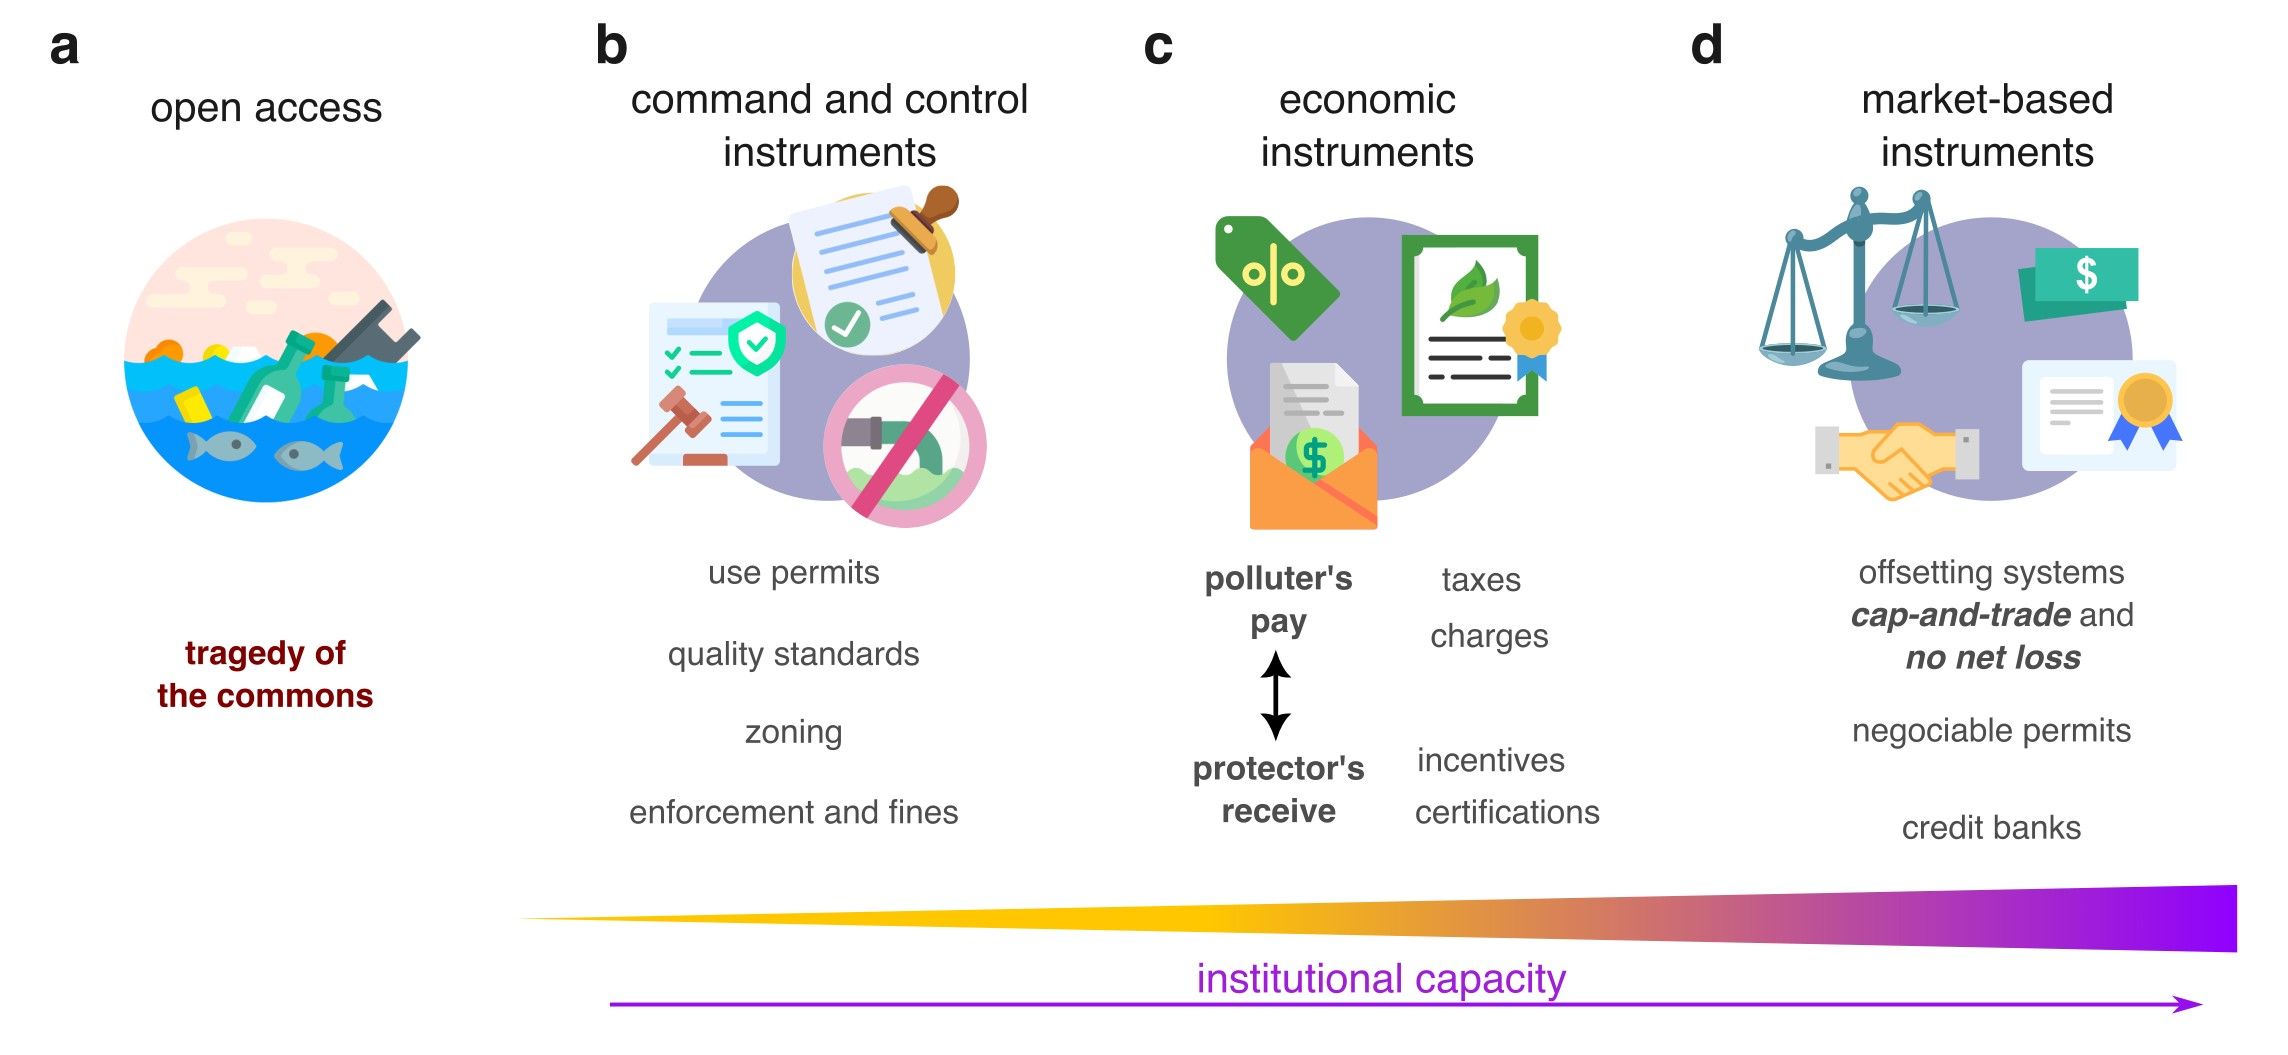
\includegraphics[width=0.98\linewidth]{figs/fig_opensacc_en.jpg}		
\caption[Solutions to the Tragedy of the Commons]
{\textbf{---\;Solutions to the \gls{probfreeacc}.}
    The tragedy of the commons arises with common resources that lack institutionalized exclusivity. The solution involves incremental layers of management instruments, requiring greater institutional capacity from the State.
    \;\textbf{a}\;---\;Without regulations on the use of common resources, individual action leads to a race to exploit natural services and raw materials, producing the tragedy of the commons — an environmental collapse.
    \;\textbf{b}\;---\;Command-and-control instruments are the first layer of management, setting general rules enforced by law on economic agents, such as usage permissions, quality standards, zoning, and penalties for infractions.
    \;\textbf{c}\;---\;Economic instruments form the second layer of management, encouraging economic agents to change their behavior beyond the mandatory general rules. Here, both the polluter-pays principle, with taxes and fees, and the protector-receives principle, with incentives and certifications, can be applied.
    \;\textbf{d}\;---\;Market-based instruments form a third layer of management, creating a negotiation space for usage permissions, allowing economic agents to find optimized arrangements on their own. In this approach, compensation systems are typically established, creating a market of credits and debits, such as cap-and-trade and no net loss. Banks are necessary to facilitate and reduce transaction costs.
}
\label{fig:eco:tragedy} 		
\end{figure}

\par Designing resource allocation policies to keep the \gls{antroposf} within its \gls{ecolimit} invariably involves addressing the \textbf{\gls{probfreeacc}}. This issue was articulated in the article \textit{The Tragedy of the Commons} by ecologist Garret Hardin (1968) \cite{Hardin1968a}. In this article, Hardin argues that environmental problems, such as land overuse and water pollution, are consequences of unrestricted access to goods and services that are commonly used, or \textbf{\gls{reccom}}\footnote{This term refers to both \gls{natcap} and \gls{antcap}.}. As individuals and companies act solely to maximize their own well-being, unrestricted access ultimately creates a rush to exploit the resource, which ends up being congested or depleted. It becomes a tragedy, therefore, as the supposedly rational actions of individuals turn into irrational collective behavior. Hardin thus recognizes that treating public resources similarly to private goods can be an interesting solution, though it does not apply in all cases:

\begin{adjustwidth}{100pt}{0pt}
\medskip
\small The tragedy of the commons as a food basket is averted by private property, or something formally like it. But the air and waters surrounding us cannot readily be fenced, and so the tragedy of the commons as a cesspool must be prevented by different means, through coercive laws or taxing devices that make it cheaper for the polluter to treat their pollutants than to discharge them untreated. We have not progressed as far with the solution to this problem as we have with the first. Indeed, our particular concept of private property, which deters us from exhausting the positive resources of the earth, favors pollution. The owner of a factory on the bank of a stream—whose property extends to the middle of the stream—often has difficulty seeing why it is not their natural right to muddy the waters flowing past their door. The law, always behind the times, requires elaborate stitching and fitting to adapt it to this newly perceived aspect of the commons. -- Garret Hardin (1968, p. 1245) \cite{Hardin1968a}.
\medskip
\end{adjustwidth}

\noindent The problem of water and air pollution can be addressed by ensuring that polluters take full responsibility for their waste. A central concept in Neoclassical Environmental Economics, in this regard, is \textbf{\gls{external}}, which can be either positive or negative. Externality refers to the impact of one economic agent's actions on the well-being of others \cite{Mankiw2002a}. In Hardin's example, where a factory pollutes the air and water, regulatory mechanisms should be created to prevent the loss of collective well-being (the negative \gls{external}), forcing the factory to manage its waste, even if it incurs higher costs. In this context, \gls{ecoeco} provides a broader interpretation of \gls{probfreeacc} and externalities compared to Neoclassical Environmental Economics. The concept of negative \gls{external}, according to this perspective, is related to the \gls{opcost} of the expansion of the \gls{antroposf} over the \gls{biosf}. Transforming a river into an effluent channel generates a series of negative externalities precisely due to the loss of \gls{natcap} — the resources and services directly provided by the river, ranging from the supply of drinking water to cultural activities.

\par Here, the concepts of \textbf{\gls{rivalty}} and \textbf{\gls{exclusvty}}, also from \gls{microeon}, are relevant for conceiving appropriate allocation policies. \textbf{\gls{recrival}} exhibit an intrinsic characteristic that prevents their use by multiple economic agents simultaneously. This interpretation is quite intuitive: if a bakery consumes flour from a silo, it automatically prevents another bakery from doing the same; if a fishing boat catches a school of fish, it automatically prevents another boat from doing the same; if a farmer plants corn on a plot of land, they prevent another from grazing sheep on the same plot. All rival resources are excludable, but not necessarily exclusive. This is because \textbf{\gls{recexclu}} require a social guarantee of reserved use by a given economic agent, which does not always exist. \gls{exclusvty} gives rise to markets, as it turns \gls{recrival} into \textbf{\gls{rectrad}}, encouraging economic agents to allocate resources among themselves based on their \gls{exchaval}. The guarantee of \gls{exclusvty} manifests essentially through \textit{deterrence} among economic agents. In small-scale societies, like families and clans, this deterrence can occur through tacit agreements. In larger societies, where strangers interact, the State tends to guarantee the right of use through a monopoly on force and the diffusion of cultural norms of coexistence. The right to \textbf{\gls{privprop}} is an institution created by the State to confer exclusive use of a rival resource to the owner, through an official document. To negotiate the resource, one must also negotiate the State’s official document that establishes \gls{exclusvty}. The difference between \gls{privprop} and a public concession is that property is lifelong and hereditary, though both are exclusivity guarantees provided by the State. In large societies with weak States, \gls{exclusvty} can also occur but often requires greater investment in private deterrence mechanisms, such as fences, weapons, and hiring mercenaries.

\par All \gls{recstflow} are rival, and all \textbf{\gls{recnonrival}} are fund-services. Since \gls{recstflow} are destroyed during their use, they are inherently rival — the same coal burned by one power plant cannot be burned by another. By definition, \gls{recnonrival} are those that can be consumed by more than one economic agent \textit{simultaneously}. Logically, therefore, these resources cannot be \gls{recstflow}. They are \gls{reccom}, for general use, accessible by all at the same time and not exhaustible or storable. A typical non-rival resource is solar radiation, a free energy flow that is relatively homogeneously distributed. If a plant photosynthesizes with sunlight, it does not automatically prevent other plants from also photosynthesizing at the same time. Another typical example is transportation routes, such as roads and highways. If a car drives on a road, it does not prevent another car from driving at the same time. Likewise, the scenic beauty of parks and beaches offers well-being to users indiscriminately.

\par The \gls{probfreeacc} can be divided between its mild form, involving \gls{recnonrival}, and its severe form, involving \gls{recrival}. \gls{recnonrival}, being necessarily \gls{fundserv}, are considered \textbf{\gls{reccongest}} because they can be consumed up to the limit of their provision rate. Congestion, as a mild form of \gls{probfreeacc}, occurs when the resource is neither destroyed nor degraded during use but imposes a maximum number of users. Typical examples occur when very tall buildings block sunlight for shorter buildings; when the road \gls{system} becomes overcrowded with the number of cars; or when parks and beaches are crowded with people seeking leisure. In all these cases, the services provided by the resources eventually lose their \gls{useval} due to unrestricted access. In such cases, the solution to the problem inevitably involves \textbf{\gls{instrcc}}, coercive impositions by the State through the action of regulatory authorities, along with auxiliary strategies such as reinforcing cultural norms.

\par The severe form of \gls{probfreeacc} occurs in the context of rival \gls{reccom}, as their uncontrolled consumption not only causes congestion but can lead to environmental collapse — Hardin's \say{tragedy of the commons} mentioned above. This is evident with stock-flow types of \gls{reccom}, such as when river water is used as an input in production processes. In this situation, unrestricted access may lead economic agents to use up all available water resources, creating scarcity and associated negative \gls{external}. However, river water can also serve as a public fund-service, as in the case of pollution. Here, the river's capacity for dilution and self-purification of waste is an example of a \textit{rival} fund-service. The river itself is not transformed into any new product, but the natural service of regulating environmental quality is progressively degraded as it is used. When an industry discharges waste into the river, the original dilution capacity is consumed, preventing subsequent industries downstream from using the service simultaneously.

\par The solution to the severe problem of unrestricted access also involves implementing some form of \gls{exclusvty} through the official issuance of \textbf{\gls{usepermits}} for economic agents \cite{Schlager1992}. Usage permits for \gls{reccom} are not \gls{privprop}, which would imply lifelong and hereditary rights of use; instead, they resemble public concessions, periodically reviewed and renewed by regulatory institutions. In the case of water, official permits for withdrawal establish \gls{exclusvty} within predefined limits, compatible with the natural availability of water sources. Similarly, official permits for effluent discharge aim to regulate the use of dilution capacity, again limiting users. Thus, allocation policies can range from conventional \gls{instrcc}, which establish general rules, to \textbf{\gls{instecon}} that not only impose penalties for negative externalities (\textbf{polluter-pays principle}[todo:gls]) but also offer incentives for users who generate positive externalities (\textbf{protector-receives principle})[todo:gls]. An advancement in this direction is \textbf{\gls{instrmarkt}}, or cap-and-trade policies \cite{Borghesi2013}. In this type of regulation, resources retain their public nature, but \gls{usepermits} are defined by exclusive quotas that can be freely traded among economic agents. A classic example of this instrument is the carbon market, where agents with credits (sequestered carbon) trade with agents with debits (emitted carbon), keeping the \gls{system} in a neutral condition \cite{Mazaheri2022}.

\par Here, it is worth noting that the development of \gls{instecon} and \gls{instrmarkt} requires a \textbf{\gls{insticap}} on the part of the State \textit{greater} than simple command and control. This is because these management policies are not merely substitutes for one another but are incrementally more complex strategies. Command and control, by itself, cannot influence economic agents beyond ensuring compliance with \textit{general rules}, such as quality standards, zoning, etc. If \gls{instrcc} goes beyond general rules, economic agents cease to exist \textit{by definition}, becoming extensions of the State itself. In societies that tolerate the existence of multiple economic agents, therefore, the State needs an extra institutional apparatus to operationalize the economic limit without making decisions for the agents. In this regard, \gls{instecon} aim to encourage behavior changes that are not mandatory but \textit{desirable}. \gls{instrmarkt} go further, with greater potential to maximize the total \gls{econbenefit}, as negotiations tend to find an optimized allocation solution within the predefined limits. In the case of pollution, the regulatory and enforcement apparatus forms a command-and-control base that cannot be abandoned, as it sets discharge standards, monitors, and applies penalties. On top of the command-and-control framework, an incentive system can be created to further reduce the use of natural services, such as encouraging water reuse. However, maintaining and updating a \textbf{credit bank} requires a higher administrative burden than just the previous enforcement apparatus. Finally, a permit market can be implemented, but not without the advent of an institution to enable and regulate its dynamics, reducing the embedded \textbf{\gls{costtransac}} of negotiating permits.

\section{Natural services} \label{chap:ecoeco:natserv}

\begin{figure}[t!] 
\centering				
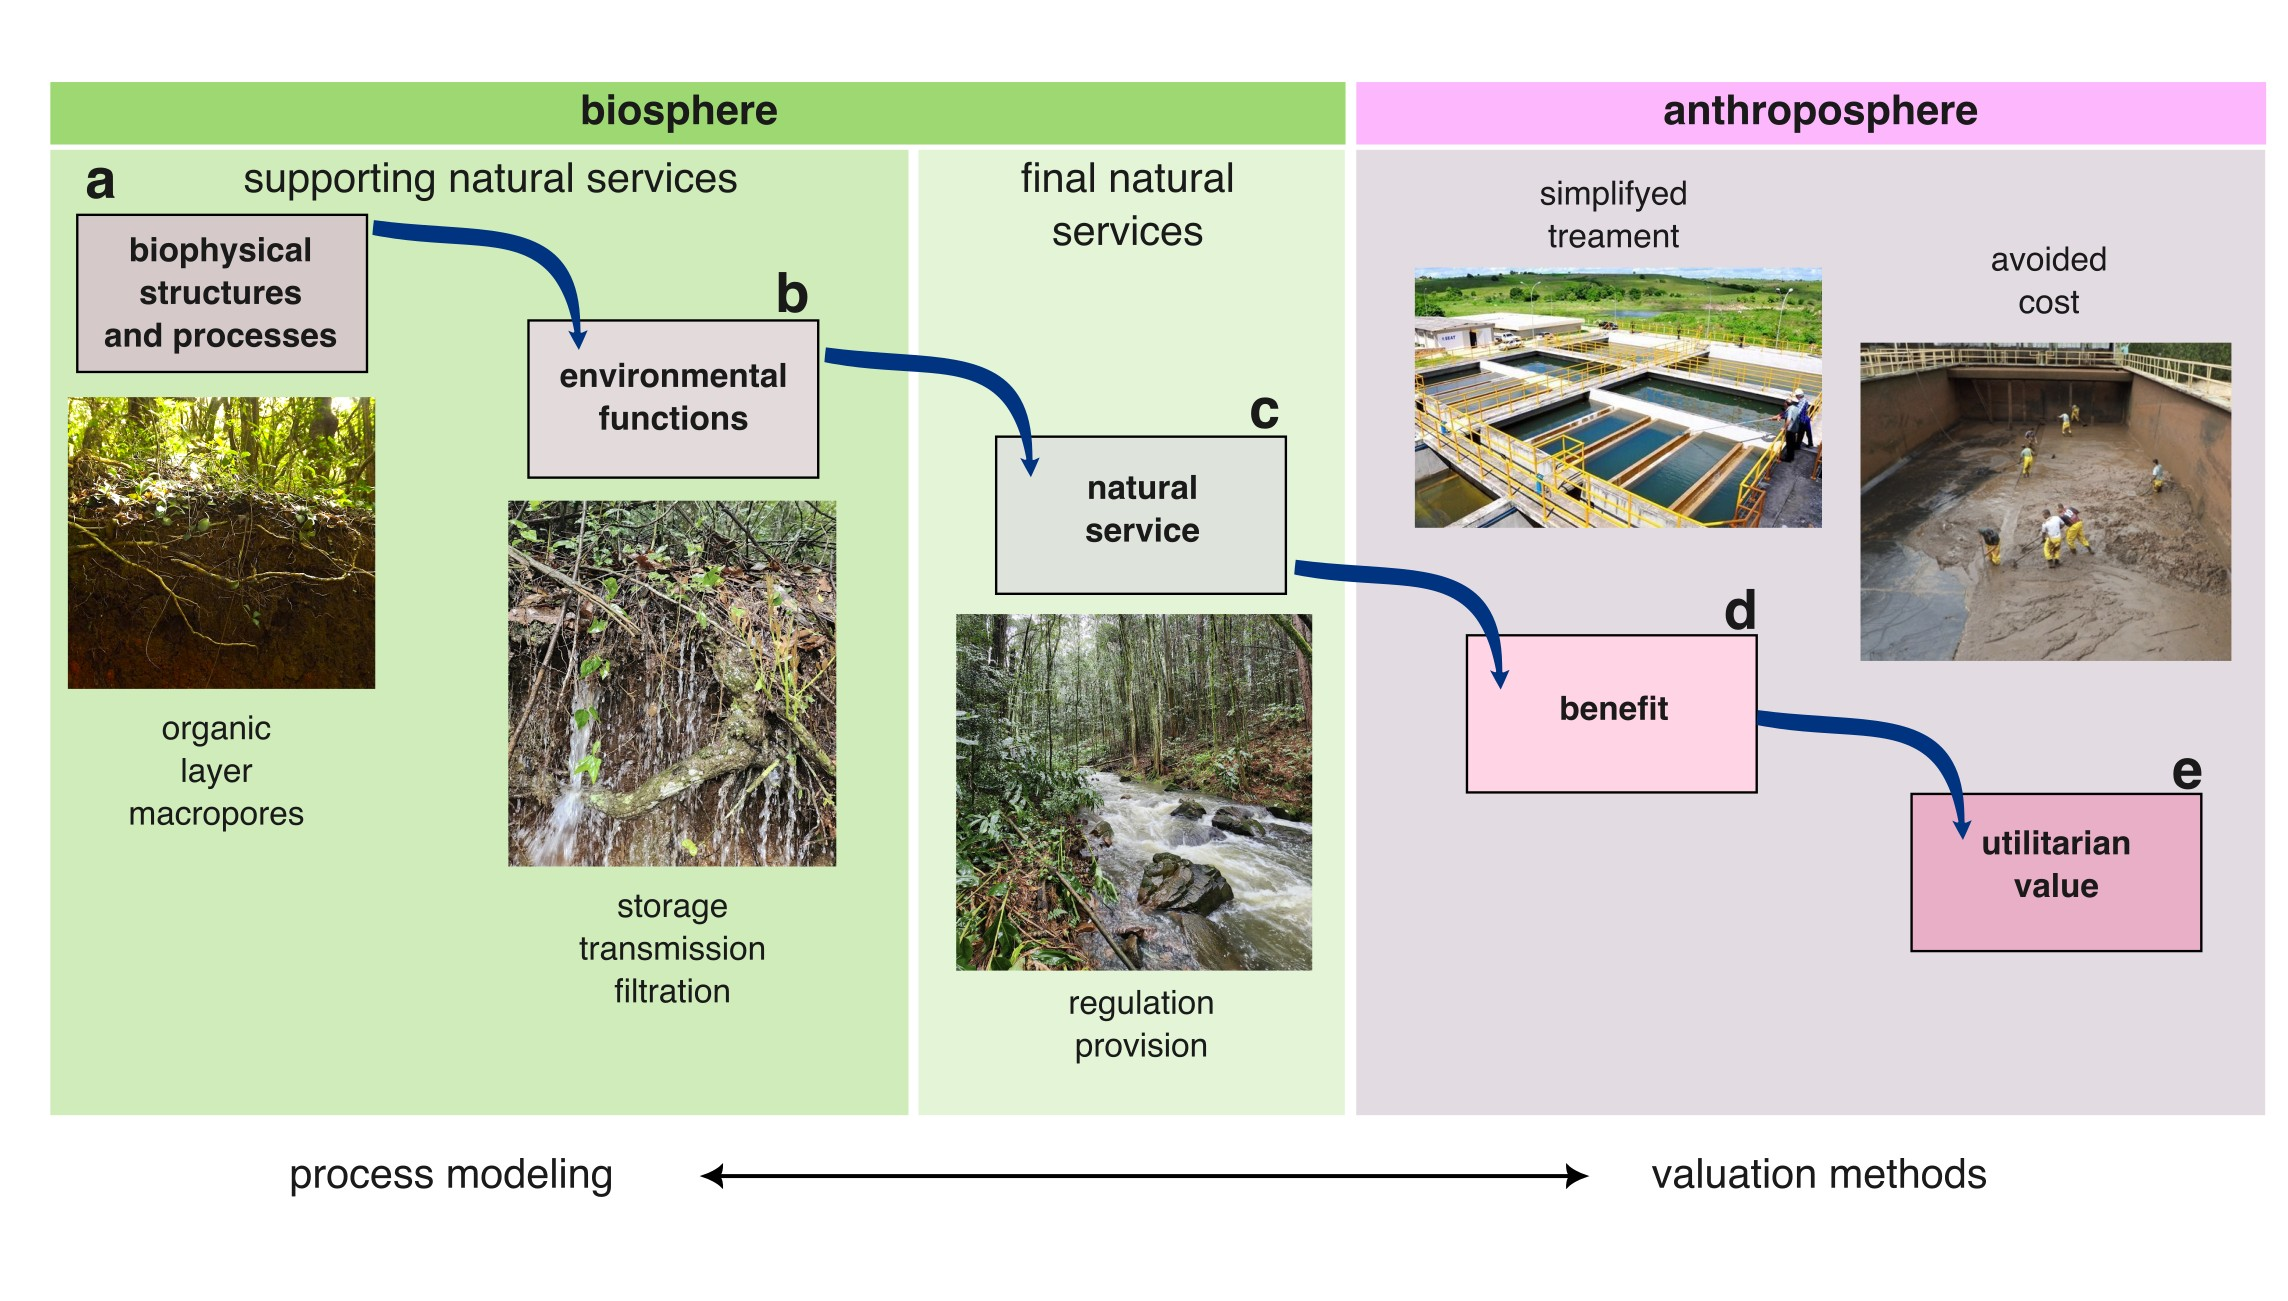
\includegraphics[width=0.98\linewidth]{figs/fig_cascade_en.jpg}		
\caption[The Natural Services Cascade Model]
{\textbf{---\;The \gls{casctmodel}.}
    The most modern conceptual framework for understanding natural services is the cascade model, proposed by Haines-Young \& Potschin (2010) \cite{haines-young2010}. This model describes how natural services flow to generate benefits for society in five stages, with the first three stages in the biosphere and the last two stages in the antroposphere. Quantitative estimates can be developed at each end through process models and valuation methods.
    \;\textbf{a}\;---\;Structural base and biophysical processes: represent the fundamental ecosystem elements that support their functions, such as physical and chemical characteristics. For example, this includes the organic horizon of the soil and the presence of macropores.
    \;\textbf{b}\;---\;Environmental functions: correspond to ecological processes stemming from structural dynamics. In the soil example, these functions encompass water storage, transmission, and filtration, essential processes for aquifer recharge and natural water purification.
    \;\textbf{c}\;---\;Final natural services: benefits derived directly from environmental functions that can be used by the antroposphere, such as providing clean water or ensuring the perennial flow of downstream watercourses.
    \;\textbf{d}\;---\;Benefit: refers to the utilitarian value derived from natural services, such as improved health, environmental security, and support for economic activities. In the case of water, one of the benefits is simplified and less costly treatment for supply.
    \;\textbf{e}\;---\;Utilitarian value: represents the economic valuation of the benefits obtained. For example, one way to assess value is by estimating the costs avoided in sludge management and advanced water treatment, or the need to source high-quality water from a more distant location.
}
\label{fig:eco:cascade} 		
\end{figure}

\par The \gls{natserv} implied by the concept of \gls{natcap} have presented both theoretical and practical challenges in designing \gls{sustdev} policies. The idea of natural service, without clear definitions, becomes intangible for influencing allocation decisions. In contrast, managing non-renewable resources is far more evident, as consuming these resources, with their irreversible destruction or transformation, makes them progressively scarce. Knowing that a coal deposit will inevitably be exhausted makes it logical to devise strategies for energy diversification. On the other hand, a tropical forest represents \gls{natcap} that provides a vast array of services, many of which are diffuse and benefit much more than just its inhabitants or visitors, at various scales. The \gls{recrenew} of the forest itself, such as timber or food, result from \gls{natservprov}, which can be degraded for various reasons, such as ecological collapse. To design management instruments for these \gls{natserv}, such as control, incentives, and trade mechanisms, they need to be identified, measured, and assigned \textbf{\gls{econval}}. This is a major challenge in the new \gls{paradigma}, even though recent advances have been made.

\par A more modern conceptual framework for understanding \gls{natserv} is the \textbf{\gls{casctmodel}}, proposed by Haines-Young \& Potschin (2010) \cite{haines-young2010, potschin2016}. This \gls{model} describes how ecosystem services flow from nature to benefit society in five main stages: (1) structure and process; (2) function; (3) service; (4) benefit; and (5) value. The first three stages belong to the \gls{biosf}, highlighting the primary importance of \textbf{\gls{biophysistrc}}, such as forests and wetlands, which provide the foundation for the development of \textbf{\gls{ecoprocess}}, such as water infiltration and nutrient cycling. These processes, in turn, generate \textbf{\gls{envfunc}} that can become useful to humans. Thus, the \gls{model} emphasizes that an ecosystem's environmental function, that is, its \textit{capacity} to do something potentially useful for humans, is not automatically a natural service. Only when this function is considered \textit{beneficial} to society does it become a service, such as the \gls{gutility} of flood regulation in densely populated areas. The last two stages of the cascade, on the other hand, belong to the \gls{antroposf}. The \textbf{\gls{econbenefit}}, therefore, corresponds to the tangible manifestation of \gls{welbeing} derived from this natural service, such as a city being less vulnerable to flood impacts. But the perception of this well-being depends on context and specific human needs, leading to variability in the assessment of its \textbf{economic value}. For example, value varies according to supply and demand conditions: during a rodent population explosion, the \gls{econval} of \gls{natservcontrol} is much higher than in normal periods. Furthermore, not all benefits can be assessed in terms of \gls{exchaval}, exhibiting only \gls{useval}, as in the case of \gls{natservcult}, which directly impact subjective well-being without intermediate material products.

\subsection{Classifications of natural services} \label{sec:natserv:sist}

\begin{figure}[t!] 
\centering				
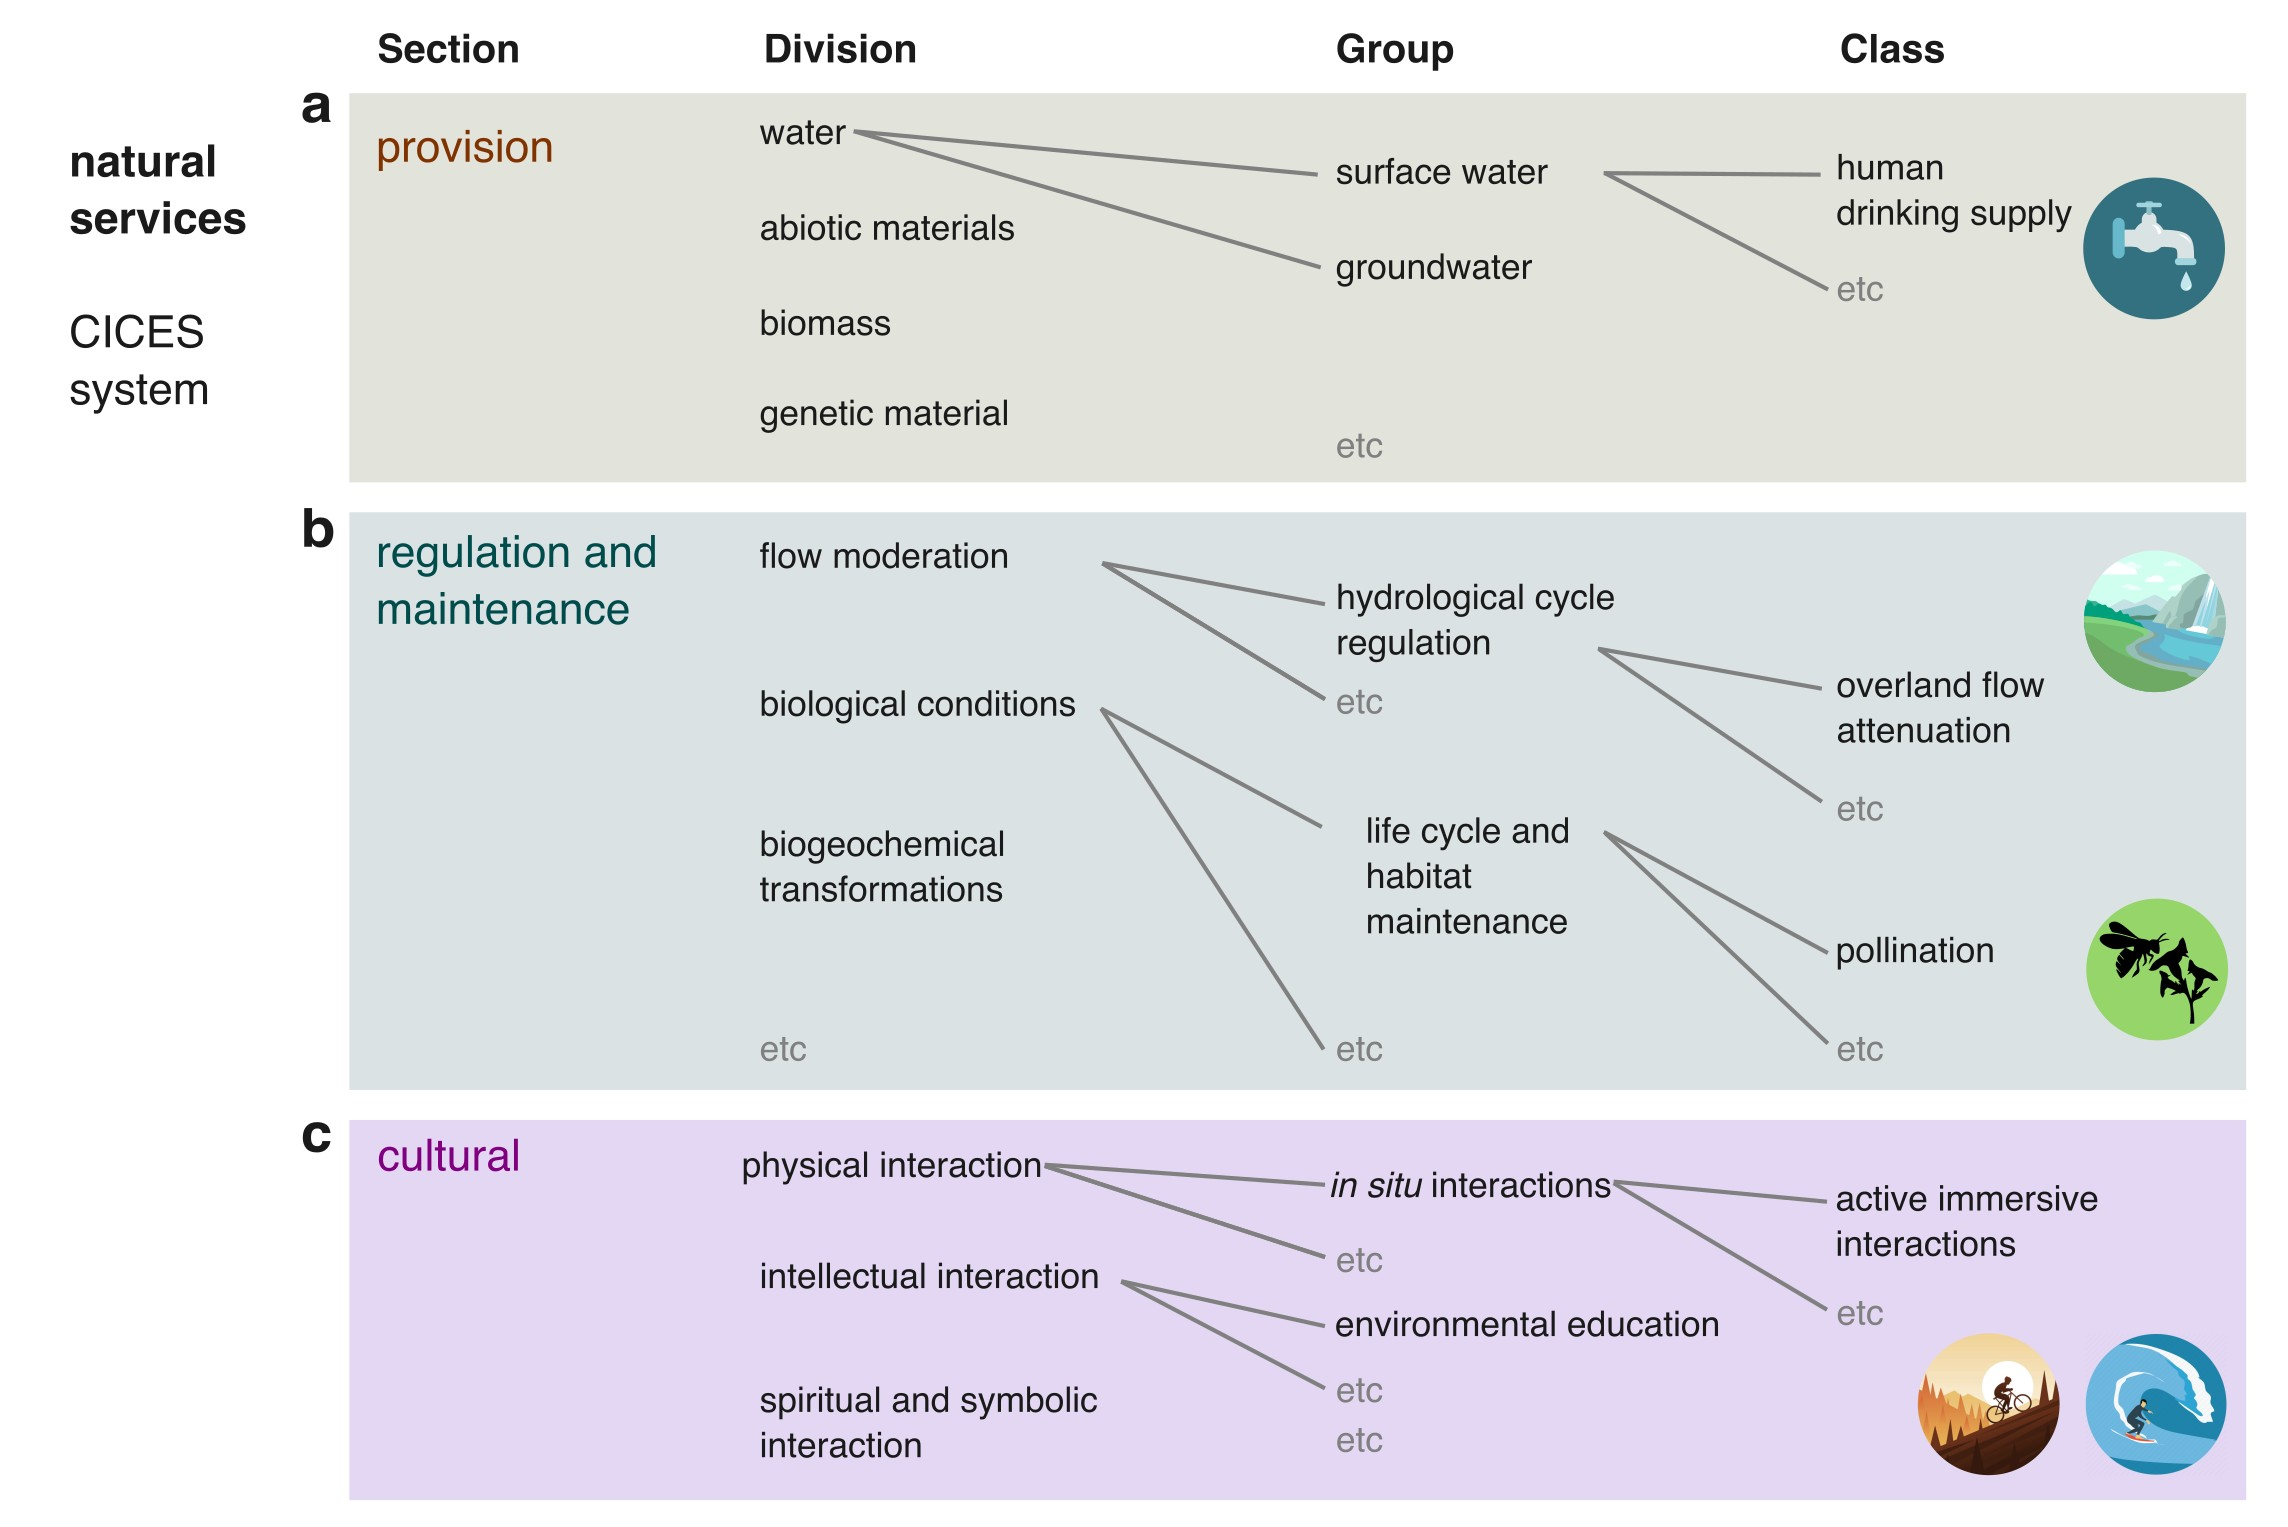
\includegraphics[width=0.98\linewidth]{figs/fig_cices_en.jpg}		
\caption[The CICES Classification System for Natural Services]
{\textbf{---\;The CICES Classification System for Natural Services}
    The Common International Classification of Ecosystem Services (CICES) provides a system categorizing ecosystem services into three main sections: provisioning, regulation and maintenance, and cultural. Each section is further detailed into divisions, groups, and classes.
    \;\textbf{a}\;---\;Provisioning natural services are related to the direct supply of raw materials (stock-flows), such as water and biomass, essential for human supply and other economic activities. For example, water is classified into subgroups like surface water and groundwater, providing essential resources for human consumption, agriculture, etc.
    \;\textbf{b}\;---\;Regulation and maintenance natural services include fund-services from biogeochemical processes and functions that ensure environmental quality and the functioning of natural cycles. These services encompass regulation of the hydrological cycle, such as flood control, and habitat maintenance for various species, like pollination.
    \;\textbf{c}\;---\;Cultural natural services represent services that provide immaterial fund-services related to physical, intellectual, spiritual, and symbolic interactions between humans and nature. These services include recreational activities, such as interactions within the natural environment, and opportunities for environmental education, promoting well-being and cultural enrichment.
}
\label{fig:eco:natserv:cices} 		
\end{figure}

\par The systematization of \gls{natserv} began with Daily \textit{et al.} (1997), especially in terms of identifying and characterizing \gls{natserv}, but also regarding valuation issues \cite{daily1997}. The authors define these services as \say{the conditions and processes through which natural ecosystems, and the species that comprise them, sustain and enhance human life}. They provide a pioneering categorization, though without including details on cultural aspects, which separates \textbf{\gls{natservgen}} from \textbf{\gls{natservbiome}}. For general services, the list includes \textbf{\gls{natservclim}} provided by various biogeochemical cycles (such as carbon, nitrogen, phosphorus, and sulfur) and sediment cycles in water. In this list, biodiversity is cited as a critical factor for ecosystem stability, ensuring greater resilience to disturbances. Also mentioned are \textbf{\gls{natservsoil}}, such as the regulation of the \gls{hydro_cicle}, physical support and nutrient provision for plants, as well as organic matter decomposition, which recycles nutrients and prevents pathogen proliferation. Other general services cited include \textbf{\gls{natservpol}}, which supports agricultural production, and \textbf{\gls{natservcontrol}}, provided by predators and parasites that reduce the need for pesticides, preserving food production stability. Biome services, on the other hand, perform all the mentioned general services but with specific uniqueness across different ecosystems. These include services from oceans, freshwater services, forest services, and natural grassland services.

\par Another historical milestone for the theoretical and practical consolidation of the \gls{natserv} concept was the \textit{Ecosystems and Human Well-being} report, a United Nations initiative completed in 2005, also known as the \acrfull{mea} report\footnote{Millennium Ecosystem Assessment, in a free translation from English.} \cite{MEA2005a}. This report advanced, to some extent, the global modeling effort of \gls{natrec} published in 1974 by the Club of Rome in \textit{Limits to Growth} \cite{meadows1974}, providing more detailed data on ecosystem distribution and changes. At the time, the assessment highlighted that approximately 60\% of \gls{natserv} were being degraded or used unsustainably, endangering the well-being of populations worldwide, especially the most vulnerable. Besides providing extremely relevant sizing, the \acrshort{mea} report helped consolidate the definition of \gls{natserv} as \textit{the direct benefits people obtain from nature}. It is worth noting that the \acrshort{mea} report also solidified the term \textbf{\gls{ecoserv}}, which is currently the most used, although there are variations like \textbf{\gls{envserv}}\footnote{Personally, I prefer the term \say{natural service}, not only because it is more comprehensive but also because it is simpler for the general public to understand.}. This terminological separation is not yet entirely clear in \gls{teoria}, but there are practical and regulatory differences. In Brazil, for instance, the National Policy on Payment for Environmental Services makes the separation as follows:

\begin{adjustwidth}{100pt}{0pt}
\medskip
\small 
(...)
Art. 2º For the purposes of this Law, the following are considered:

I - ecosystem: a dynamic complex of plant, animal, and microorganism communities and their inorganic environment interacting as a functional unit; 

II - ecosystem services: benefits relevant to society generated by ecosystems, in terms of maintaining, recovering, or improving environmental conditions, (...)

III - \gls{envserv}: individual or collective activities that favor the maintenance, recovery, or improvement of ecosystem services.

-- Brazil (2021, p. 1) \cite{brasil2021}.
\medskip
\end{adjustwidth}

\noindent Despite this official definition, the term \say{environmental service} can also refer to benefits obtained from natural elements within built environments, such as cities. In this view, urban forestry, for example, would consist of a form of \textbf{\gls{greeninfra}} that provides \gls{envserv}.

\par The \acrshort{mea} report paved the way for the systematization of \gls{natserv} currently adopted by the \acrfull{cices}, illustrated in Figure \ref{fig:eco:natserv:cices}, which was mentioned in the previous section: \gls{natservprov}, \gls{natservreg}, and \gls{natservcult} \cite{Haines-young2018a}. A fourth category was also articulated by the \acrshort{mea}, which would be \textbf{\gls{natservsup}}, but in \acrshort{cices}, services in this class were either disaggregated or conceptually maintained as precursor processes of the services themselves. The systematization proposed by \acrshort{mea} and \acrshort{cices} adopts an approach opposite to that of Daily \textit{et al.} (1997), as it takes an economic and anthropocentric perspective focused on the typology of services rather than their origin in the \gls{biosf}. This classification directly guides decisions and evaluations related to \gls{sustdev}, regardless of the ecosystems involved. In provisioning services, the main issue is whether the materials provided by the ecosystem are being consumed at a rate exceeding their regeneration capacity, as seen with soil erosion in agricultural lands or overfishing. For regulation and maintenance services, the focus is on assessing the ecosystem's capacity to regulate resources, identifying the extent to which this capacity can be used without requiring additional measures, such as soil water storage to regulate water availability or carbon absorption by oceans to mitigate global warming. For cultural services, the central question is to identify and assess the intangible benefits different groups obtain from the ecosystem, from leisure to scientific and educational value. This systematization thus emphasizes the economic aspect, facilitating policy formulation for \gls{sustdev}. Costanza (2008) suggests that this is an inevitable consequence of the transition between the \gls{biosf} and the \gls{antroposf}, making it necessary to maintain more than one \gls{system} of classification—some to map and identify services on the \gls{biosf} side and others to assist decision-making on the \gls{antroposf} side \cite{costanza2008}.

\par The \acrshort{cices} system presents a hierarchical structure that organizes \gls{natserv} into three levels: sections (highest level), divisions (intermediate level), and groups (lowest level), providing a standardization that facilitates environmental accounting and inventory. Without such a detailed \gls{system}, it would be virtually impossible to develop effective policies for the management and valuation of these services. With it, projects and actions can be explicitly focused on maximizing one or more \gls{natserv}. From a hydrological perspective, for example, water provision is a division within the provisioning service (code 4.2), which also covers the provision of biomass and other abiotic resources. This division is subdivided into groups, such as surface water provision (code 4.2.1) and groundwater provision (code 4.2.2). In the case of surface water, service classes include potable water provision (code 4.2.1.1), water provision as a material input (code 4.2.1.2), and water provision for energy production (code 4.2.1.3). These services can compete with each other, as in a reservoir supplying a hydroelectric plant, where use for energy generation may conflict with demand for potable or industrial water. Concerning regulation and maintenance services, attenuation of \gls{hydro_cicle} flows in \acrshort{cices} results from both biotic (code 2.2.1.3) and abiotic divisions (code 5.2.1.2). Biotic regulation involves hydrological processes at the hillslope scale, where fauna and flora influence surface fragmentation, enhancing infiltration. Abiotic regulation occurs at the watershed scale, such as in floodplains. Both services require management, as they can be compromised by soil compaction on hillslopes or dike construction in floodplains.

\subsection{Manifestations of utility value} \label{sec:natserv:value}

\begin{figure}[t!] 
\centering				
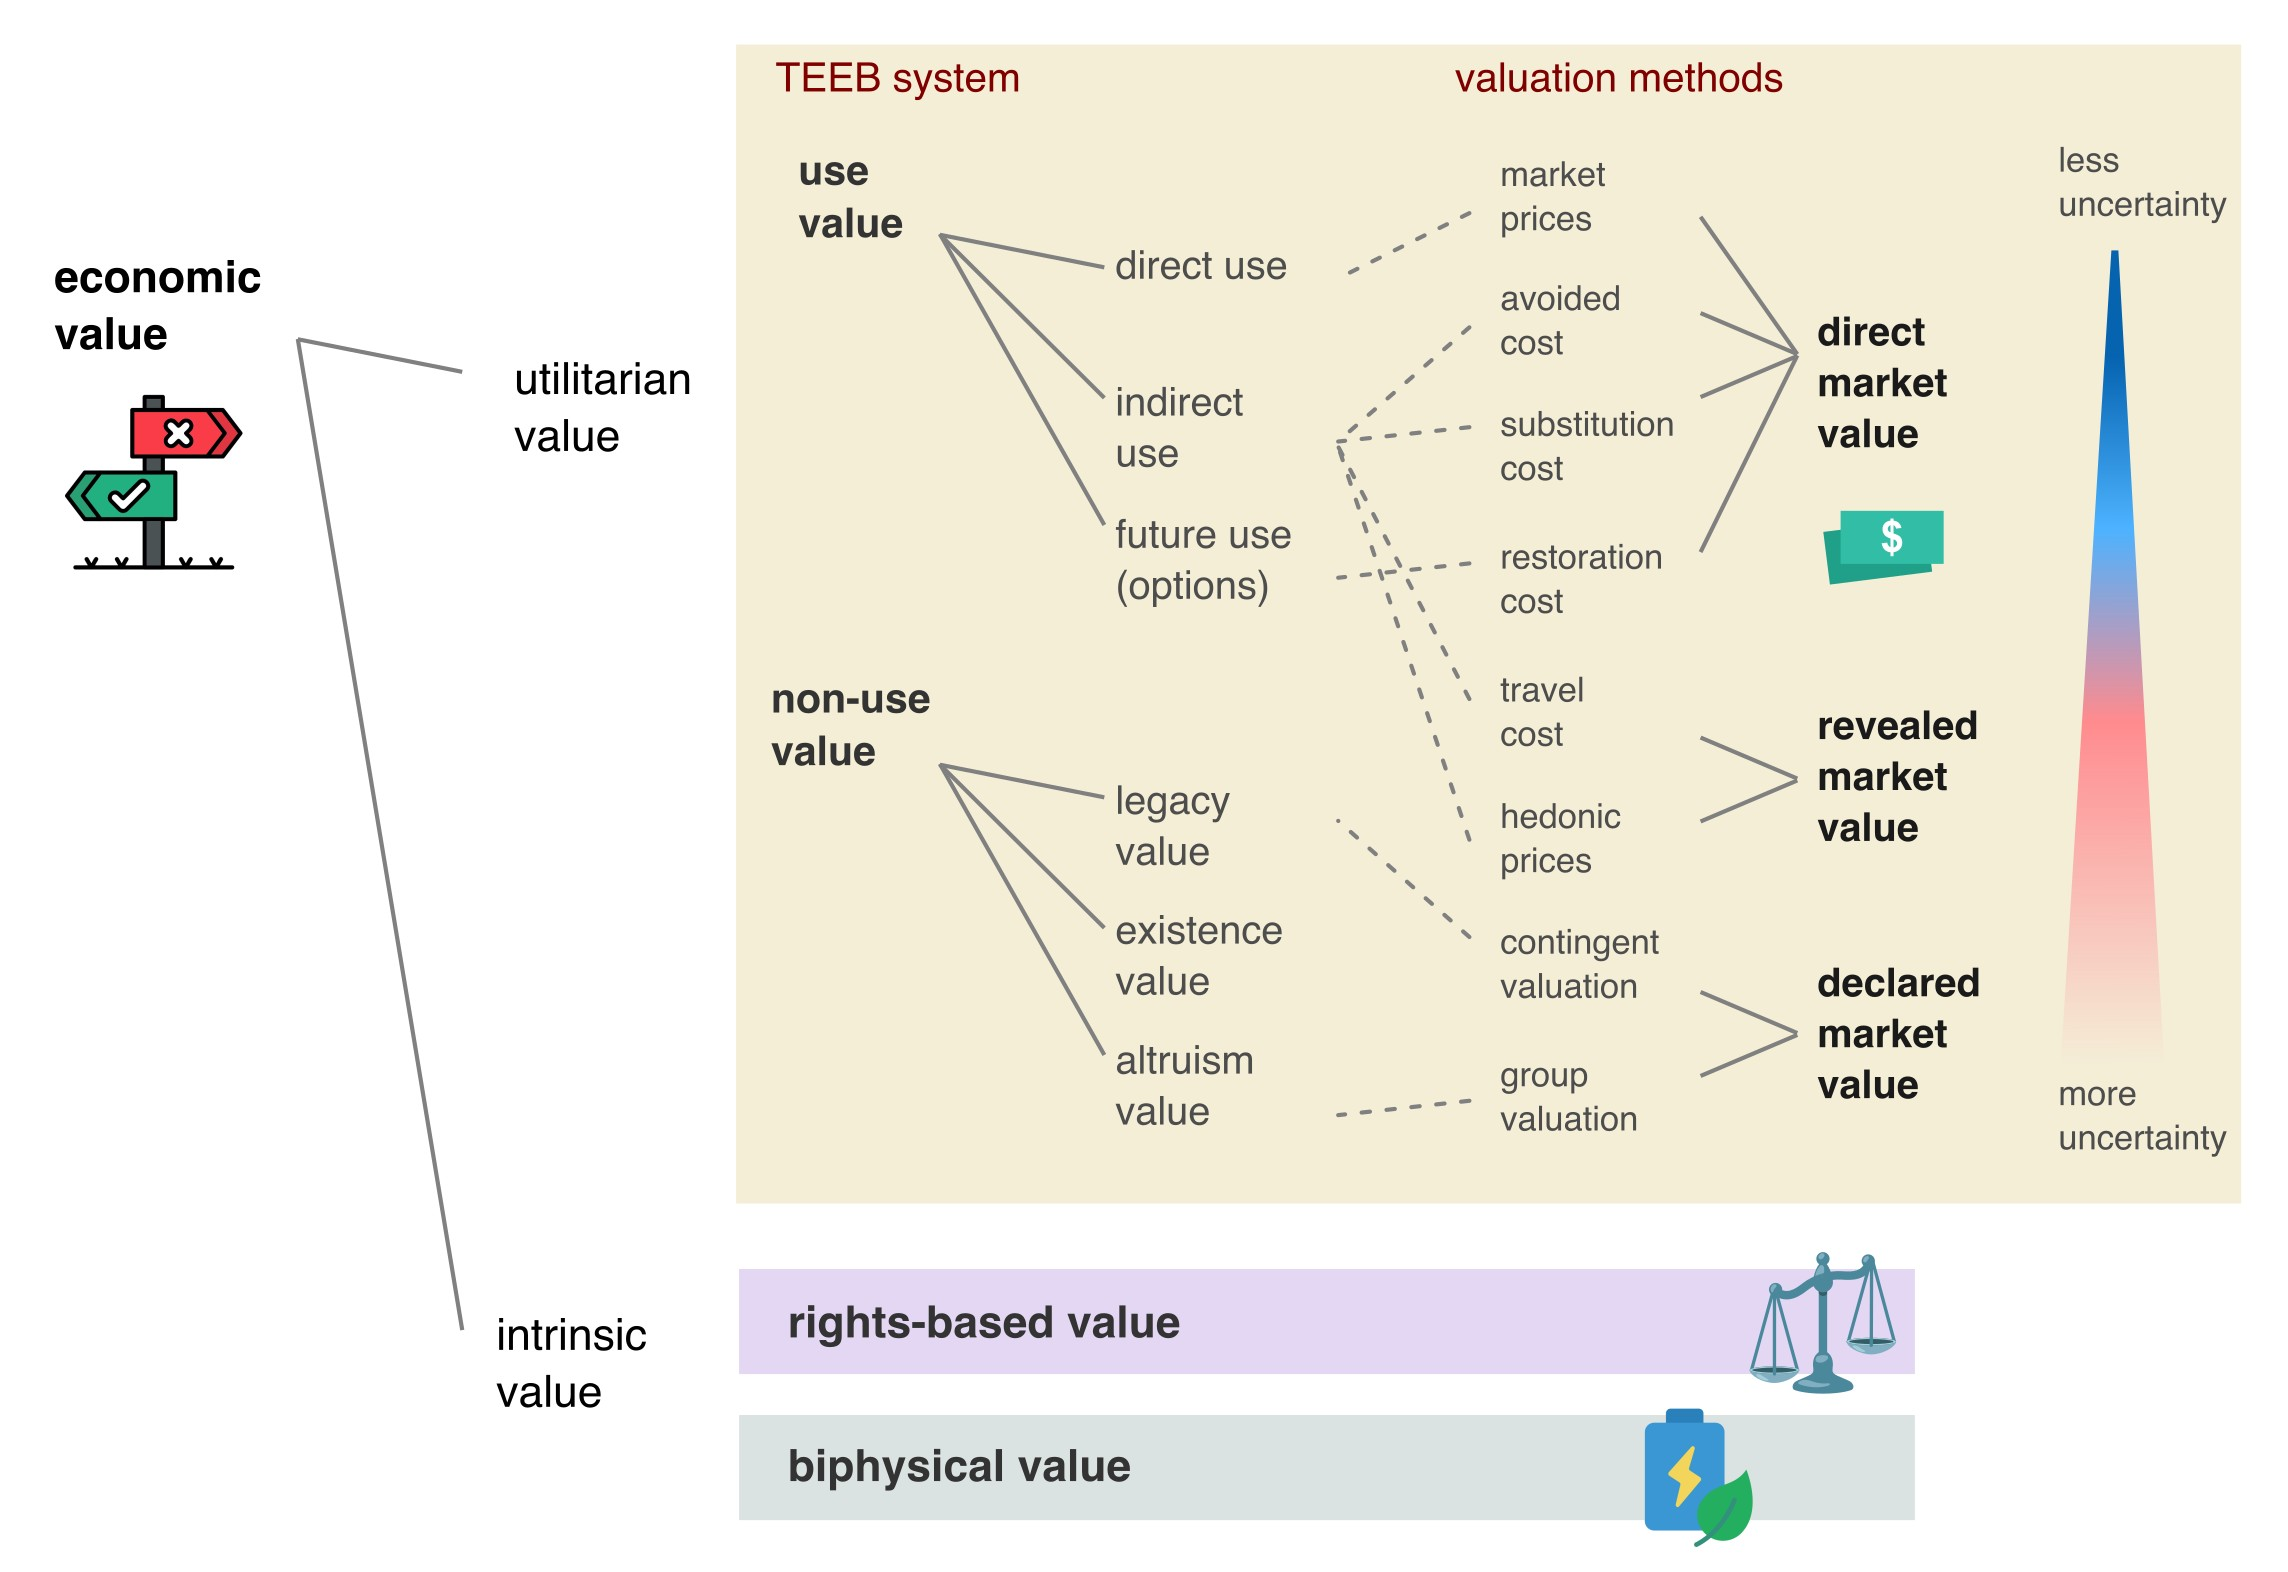
\includegraphics[width=0.98\linewidth]{figs/fig_teeb_en.jpg}		
\caption[Manifestations of Utility Value]
{\textbf{---\;Manifestations of \gls{utilval}.}
    Utility value is the metric of the utilitarian ethical paradigm, which selects the maximization of utility as its ultimate goal. However, other forms of intrinsic value are possible for guiding economic decisions, such as rights-based (deontological) value and biophysical value, like carbon footprint or water footprint.
    \;\textbf{a}\;---\;In the TEEB system, utility value involves both use and non-use value. Use value includes direct use (consumptive and non-consumptive); indirect use (with intermediaries); and future use value, also known as option value. Non-use value consists of utility values that include legacy value, existence value, and altruism value.
    \;\textbf{b}\;---\; Valuation methods include direct market value, such as prices and costs; indirect market value, like the added value of scenic beauty and the opportunity cost of tourists' time; and declared market value, when surveys are conducted to infer value in hypothetical markets. The more direct the valuation, the lower the uncertainty associated with the method.
}
\label{fig:eco:natserv:value} 		
\end{figure}

\par The valuation of \gls{natserv} involves the last two stages of the cascade model: benefit assessment and \gls{econval}. To fully understand this process, it is necessary to step back from practical aspects and revisit more theoretical issues. A \textit{value} is a metric used in making choices, which are always guided by a supreme ethical objective. For instance, if honesty is an important value for human relationships, then it is \textit{better} to interact with trustworthy people than with deceitful ones (and to be honest so as not to be \textit{devalued} by others). Thus, valuation is the calculation of this metric based on predefined ethical foundations. In this sense, a value is considered \textit{economic} when it is the metric for allocating scarce resources among different ends. In \gls{ecoeco}, which is based on \gls{gutilitarism}, \gls{econval} is a \textbf{\gls{utilval}}—the \gls{gutility} or sense of \gls{welbeing}. Thus, despite all the differences resulting from adopting a physicalist ontology, \gls{ecoeco} aligns with the Neoclassical economic paradigm in its ethical dimension. Both consider \gls{gutility} as the \gls{ultimategoal}, though the former recognizes its physical limit while the latter does not.

\par However, \gls{utilval} is not the only possible way to assess choices in an economic context, as there are also forms of \textbf{\gls{intrisval}}, based on rights or biophysical properties \cite{kumar2012economics}. The \textbf{\gls{rightval}}\footnote{Also known in philosophy as deontological value, as it is not consequentialist but based on rules defined \textit{a priori}.} seeks to correct the \gls{antropoc} inherent to \gls{gutilitarism}, which, for example, does not explicitly ensure that other species are not driven to extinction, provided that this does not detract from the overall \gls{welbeing} calculation. An alternative to this approach is \textbf{\gls{gbiocentrism}}, inspired by Kantian ethics, which asserts that other species have the inalienable right to exist. In this context, Kant's \textbf{\gls{impercateg}} serves as a moral principle that should be followed regardless of utilitarian consequences. This ethical principle states that decisions should be made \textit{as if} they were derived from a \textit{universalizable} law. Thus, this logic can be applied to establish the rights of other species, since if we dislike the idea of being used or exterminated by technologically superior species, we should not do this to less advanced species \cite{daily1997}. The \textbf{\gls{biophyval}} uses physical metrics, such as embodied energy and materials, to decide on resource allocation. This value is an extended version of \textbf{labor value} as identified in Karl Marx's economics. The concept of \textbf{\gls{ecofootprint}}, for instance, assigns value based on the material load required to produce a good or service, such as carbon and water footprints. These valuations, though philosophically distinct, are not mutually exclusive and can complement each other through \textbf{\gls{amcrit}} or multi-objective optimization. Biocentric rights, for example, can function as constraints on the extent of utilitarianism, while life cycle analysis can influence the sense of satisfaction or \gls{welbeing}. After learning about the substantial carbon footprint of an airplane trip, you might be willing to pay an extra fee to offset emissions.

\par The possible manifestations of \gls{utilval} for \gls{natserv} are systematically explored by the \acrfull{teeb} initiative, illustrated in Figure \ref{sec:natserv:value}. The authors of this initiative define \textbf{\gls{tev}} as the sum of all forms of \gls{utilval}, organized into a hierarchy of values. It is worth noting that this is a broad conceptual \gls{system}, applicable to both natural and anthropogenic capital. While obtaining the total value of a given resource is challenging and uncertain, this is often unnecessary for decision-making, as economic agents usually focus on specific components of this value. At the same time, from a \gls{natcap} management perspective, the \gls{tev} concept is crucial in reminding us that management solutions must consider the trade-offs between agents involved in different components.

\par The \gls{tev} is divided into \textbf{\gls{useval}} and \textbf{\gls{nonuseval}}. \gls{useval}, as previously mentioned, is a relatively intuitive and well-established concept in \gls{gseconomics}. The \gls{marutilteo} suggests that marginal use value—the incremental benefit obtained per unit consumed—corresponds to the \textbf{exchange value}, which varies according to supply and demand in efficient markets. On the other hand, \gls{nonuseval} refers to the satisfaction and well-being derived from \textit{not} using a given good or service. Although less tangible, these values cannot be ignored and include \textbf{\gls{legval}}, reflecting concern for resource availability for future generations; \textbf{\gls{altrval}}, which considers equity among members of the current generation; and \textbf{\gls{existval}}, relating to satisfaction derived simply from knowing that species and ecosystems continue to exist.

\par \gls{useval} includes both \textbf{\gls{direcuseval}} and \textbf{\gls{indirectuseval}}. \gls{direcuseval} refers to explicit interaction with the resource, whether it is a natural service or a conventional consumption good. This direct use can be \textbf{\gls{useconsum}} or \textbf{\gls{usenonconsun}}. \gls{useconsum} involves the irreversible transformation of the resource, as is the case for all stock-flow resources. \gls{usenonconsun}, on the other hand, is more related to fund-service resources, which are not transformed. Going to the movies, for example, involves \gls{direcuseval} with \gls{useconsum} (the popcorn) and \gls{direcuseval} with \gls{usenonconsun} (the movie itself). In the context of \gls{natcap}, \gls{natservprov} offers resources with \gls{direcuseval} and \gls{useconsum}, while \gls{natservcult} provides \gls{direcuseval} and \gls{usenonconsun}. A river supplying drinking water to a city, for instance, has \gls{direcuseval} with \gls{useconsum} because the water is transformed in the process. However, recreational activities on the same river have \gls{direcuseval} with \gls{usenonconsun}. \gls{indirectuseval}, on the other hand, refers to less explicit interactions with the resource, where the value is realized through intermediary processes often not immediately visible. Using the cinema example, we seldom interact directly with the cleaning staff, but a clean environment enhances our experience. Similarly, in the context of \gls{natcap}, indirect use is associated with \gls{natservreg}. Pollination by insects, for instance, is essential for agriculture, but this service does not involve direct interaction between the food consumer and the pollinators. Similarly, water infiltration on hillsides benefits downstream users by providing clean water, even if they do not interact directly with the natural process.

\par \gls{direcuseval} and \gls{indirectuseval} are both forms of \gls{useval} \textit{in the present}. However, the authors of \acrshort{teeb} also highlight a form of \textbf{\gls{futuseval}}, known as \textbf{\gls{optionval}}. This value, in the context of \gls{natcap}, is strongly tied to ecosystem resilience and recovery from disturbances. However, this resilience has limits and may be compromised when the ecosystem undergoes a significant disturbance, surpassing a \textbf{\gls{tippingpoint}}. Beyond this critical threshold, the \gls{system} attractor moves to a new stable or unstable state, resulting in the loss or significant degradation of previously available \gls{natserv}. An example of a stable-stable regime shift is the introduction of invasive species, which quickly disrupt ecological balance and reduce biodiversity. In this situation, restoring the original ecosystem becomes extremely costly as the \gls{system} attractor has shifted to another point or region of stability. A stable-unstable regime shift, on the other hand, occurs when soil erosion progresses from small rills to large gullies and ravines, with strong positive feedback intensifying erosion over time. \gls{optionval} reflects the \textbf{\gls{riskaversv}} of regime shifts in the \gls{system}, which would entail exorbitant costs. In this context, \gls{uncert-episteme} — the lack of knowledge about the \gls{system} — becomes a crucial factor in assessing this value, increasing as ignorance of the \gls{system} behavior is recognized. \gls{futuseval}, therefore, is directly linked to the \textbf{\gls{precauprinci}}, which advises that, under high uncertainty about non-return points, policies should be guided by conservative safeguards.

\subsection{Valuation methods} \label{sec:natserv:valuemethos}

\par Determining each component of the \gls{tev} involves using various methods that proceed incrementally, according to available information on marginal \gls{useval} (prices). Naturally, technical, methodological, and uncertainty limitations increase as available information becomes scarcer. When \gls{natserv} are closely tied to real markets, \textbf{\gls{valuadm}} techniques can be applied. In cases where \gls{natserv} have an indirect relationship with real markets, information is sought in parallel real markets through \textbf{\gls{valuarevpref}} techniques. Finally, in the complete absence of a real or parallel market, valuation alternatives employ \textbf{\gls{valuastatpref}} techniques, estimating the value in hypothetical markets.

\par In the most basic case, \gls{valuadm} identifies market transactions directly linked to \gls{natserv}. This method is divided into three main categories: \textbf{\gls{valuaprice}}, \textbf{\gls{valuacost}}, and \textbf{\gls{valuafuncprod}}. Market \gls{valuaprice} relates to \gls{natservprov} whose products are traded in markets. This approach is as direct as possible: the direct, marginal \gls{useval} with \gls{useconsum} is the market \gls{gprice}, which may be adjusted to remove potential distortions. Cost-based approaches, more associated with \gls{natservreg}, focus on estimating the expenses required to replicate the benefits of \gls{natserv} through artificial means. These techniques include \textbf{\gls{valuaavoid}}, which considers production costs that would be incurred in the absence of \gls{natserv}; \textbf{\gls{valuarepo}}, which estimates the cost needed to replace the service itself with artificial technologies; and \textbf{\gls{valuarest}}, which evaluates the expenses required to mitigate or restore \gls{natserv}. Production function-based approaches are the most integrated methods within this category when there is enough knowledge to establish the causal link between \gls{natserv} performance and the production of a market-traded good or service.

\par In the intermediate case, revealed preference techniques rely on observing individual choices in existing markets indirectly related to the natural service in question. In other words, economic agents \textit{reveal} the \gls{gutility} of the service through their choices. \acrshort{teeb} authors emphasize that the primary methodologies in this scope are \textbf{\gls{valuatravcost}} and \textbf{\gls{valuahedonpric}}, both strongly related to \gls{natservcult} values with direct and \gls{usenonconsun} use. Travel cost estimation is essential for valuing cultural services related to tourism and recreational activities, including direct expenses and \gls{opcost} of time. Thus, the value of a change in the quality or quantity of a recreational site can be inferred from the estimated demand function for visits. In contrast, hedonic pricing uses information about the implicit demand for an environmental attribute embedded in resources traded in markets. A typical example of this \textit{added value} is the scenic beauty highly valued in property prices with views of natural landscapes. Installing wind turbines and other aspects of visual pollution in the landscape can lead to the loss of this cultural natural service, as evidenced by property devaluation.

\par Finally, in the absence of market information, stated preference approaches simulate a hypothetical market for \gls{natserv} using surveys that consider changes in service provision. These techniques can estimate both use and non-use values, such as existence or \gls{legval}. Among the available techniques is \textbf{\gls{valuacontg}}, which uses questionnaires to infer economic agents' willingness to pay for improvements in a natural service or willingness to accept degradation in a natural service—two sides of the same coin. A more complex form involves the \textbf{\gls{valuachoice}} method, where survey respondents are presented with a network of possible choices, better indicating declared loss and gain relationships. An even more robust assessment includes \textbf{\gls{valuagroups}}, where different economic agent groups participate in a pluralistic process to deliberate the value of a given service or natural resource. This process enables, with multi-criteria approaches, integration with other value metrics and ethical systems mentioned above.

\section{Watershed natural services} \label{chap:ecoeco:watersheds}

\begin{figure}[t!] 
\centering				
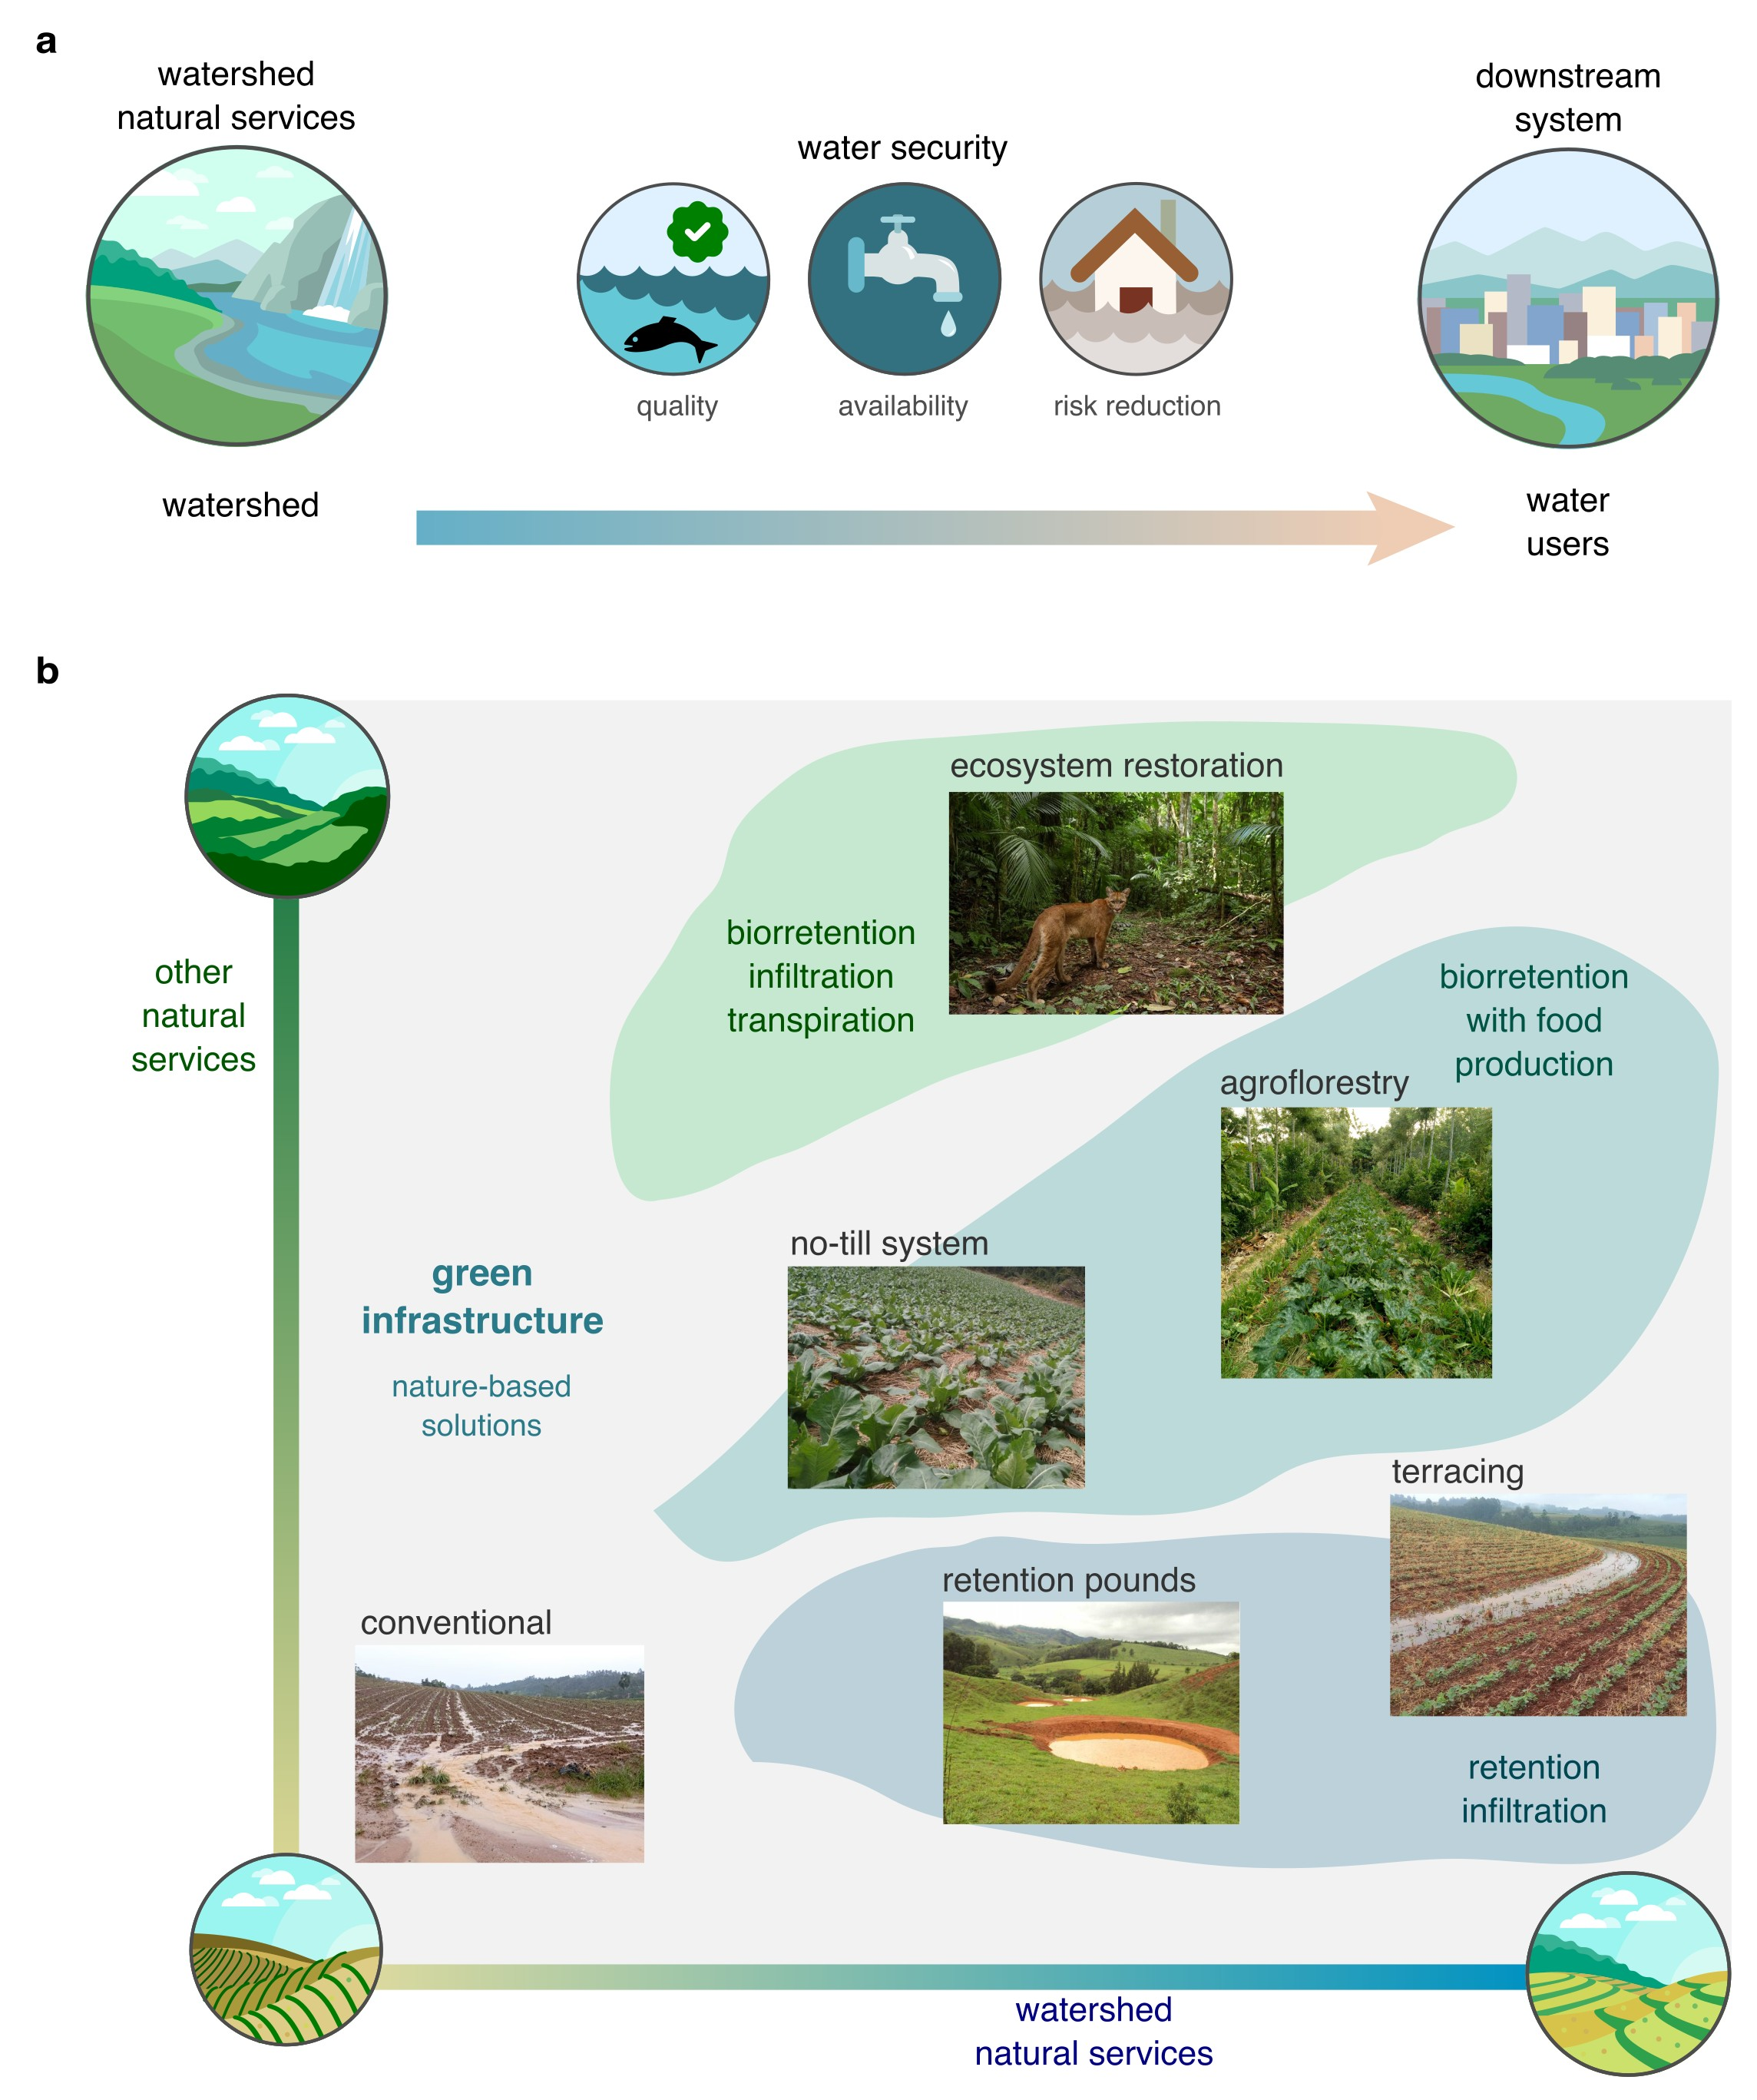
\includegraphics[width=0.98\linewidth]{figs/fig_sbn_en.jpg}		
\caption[Watershed natural services and the expansion of green infrastructure.]
{\textbf{---\;Watershed natural services and the expansion of green infrastructure.}
    Watershed natural services encompass a wide range of services related to land use, spanning from zero-order catchments to floodplains.
    \;\textbf{a}\;---\;The primary characteristic of watershed natural services is their scale of manifestation (the watershed) and their linear causal relationship, benefiting downstream water users. From an integrated water resource management perspective, watershed natural services contribute to water security by improving quality, increasing availability, and reducing risks associated with hydrological processes.
    \;\textbf{b}\;---\;Complementary to gray infrastructure, the expansion of various forms of green infrastructure, which are nature-based solutions, can enhance the provision of watershed natural services. In zero-order basins and slopes, these solutions include techniques to increase surface retention capacity and soil infiltration. Synergies and trade-offs with other natural services may arise here. For example, ecological restoration implies forgoing conventional food production. Agroforestry balances both water production and food production while also supporting natural services related to biodiversity.
}
\label{fig:eco:watersheds} 		
\end{figure}

\subsection{Water security and green infrastructure} \label{sec:watersheds:watersecurity}

\par With the advent of Ecological Economics and its concept of natural capital, new perspectives have emerged to frame \textbf{Integrated Water Resources Management} (IWRM), defined by the Global Water Partnership as “a process that promotes the coordinated development and management of water, land, and related resources, aiming to maximize the resultant economic and social welfare in an equitable manner without compromising the sustainability of vital ecosystems” \cite{GWP2000}. As a paradigm for watershed management and planning, IWRM largely aims to ensure \textbf{water security}. The United Nations defines water security as the capacity of a population to: ensure sustainable access to adequate quantities of water of acceptable quality, necessary to sustain its socioeconomic development; protect against water-related pollution and disasters; and preserve ecosystems in a context of peace and political stability \cite{cassin2021}. In practice, ensuring water security requires planning and managing programs, projects, and actions that, within socioeconomic and geopolitical contexts, guarantee the availability, quality, and regularity of water in sufficient conditions to meet the demands of multiple water users, in addition to mitigating human risks associated with extreme events, such as major floods and landslides. Such users in a watershed represent different agents or economic sectors, ranging from traditional communities and water supply companies to economic sectors such as agriculture, industry, and energy production.

\par Under the ecological-economic paradigm, water ceases to be viewed solely as a production factor for these users and is instead recognized as a common resource provided by the natural capital of the watershed. From this perspective, it becomes clear that the allocation of water for different uses actually involves the consumption of a series of natural services provided by the basin's ecosystems, referred to as \textbf{hydrological natural services}. Smith \textit{et al.} (2006) \cite{Smith2006a} demonstrate that these services go beyond the mere provision of water, also including the provision of food, regulation of water and sediment flows, water quality, mitigation of hydrological risks, and various cultural natural services (Table \ref{tbl:waterserv}). Moreover, this interpretation suggests that the economic value of water, fundamental in allocation strategies and water use charging in Brazil\footnote{In this case, by the National Water Resources Policy (Brazil, 1997)}, is actually a network of providers and consumers of the natural service of provision and regulation. If a city abstracts water from a source with good quality and availability, the value of that water is tied to the fact that the watershed is in a good state of conservation, for example. Similarly, a downstream irrigator owes part of their production to an upstream farmer who has invested heavily in soil conservation actions, such as the construction of infiltration trenches.

{\renewcommand{\arraystretch}{1.5}
\begin{table}[t!]
    \centering	
    \tiny
    \sffamily
    \rowcolors{2}{white}{rowgray}
    \begin{tabular}{ 
        >{\raggedright\arraybackslash}m{1.5cm} 
        >{\raggedright\arraybackslash}m{2.5cm}  
        >{\raggedright\arraybackslash}m{3.0cm}  
        >{\raggedright\arraybackslash}m{2.5cm}
        >{\raggedright\arraybackslash}m{2.5cm}
    }
    \toprule 
    \textbf{Service section} & \textbf{Watershed services} & \textbf{Service attributes} & \textbf{State indicator} & \textbf{Sustainable use indicator} \\ 
    \midrule 
    \textbf{Provision} & Water supply & Precipitation, infiltration, soil retention, percolation, streamflow, groundwater flow, biotic and abiotic effects on water quality & Water storage capacity (m³/m²), Pollutant concentrations & Discharge (m³/year) \\ 
    
    \cline{2-5} 
     & Food provision & Crop, fruit, livestock production, edible plants and animals (e.g., fish, algae, invertebrates) & Agricultural water use (m³/ha), Fish stock (kg/m³) & Maximum sustainable water use for irrigation (m³/year), Net productivity (kg/ha/year) \\ 
    
    \cline{2-5}
     & Non-food goods & Production of raw materials (e.g., timber, reeds), production of medicines & Amounts available (kg/ha/year) & Maximum sustainable harvest (kg/ha/year) \\ 
    
    \cline{2-5} & Hydro-electric power & Flow for energy generation & Storage capacity of riverbeds and lakes (m³/m²), Slope (degree), Elevation (m) & Maximum sustainable energy production (kWh/year) \\ 
    
    \textbf{Regulation} & Regulation of water flows & Retention of rainfall and release (especially by forests and wetlands), Water storage by rivers, lakes, and wetlands, Groundwater recharge and discharge & Infiltration capacity (mm/h), Water storage capacity of soils (m³/m²) & Baseflow volume (m³/year) \\ 
    
    \cline{2-5}
    & Hazard mitigation & Reduced flood peaks and storm damage, Coastal protection, Slope stability & Maximum natural water storage capacity (m³/m²) & Size (km²) and economic value (US\$/km²/year) are protected from flooding \\ 
    
    \cline{2-5}
    & Control of soil erosion and sedimentation & Protection of soil by vegetation and soil biota & Infiltration capacity (mm/h), Slope length (m), Barren land (\%) & Soil loss (kg/ha/year), Sediment storage (kg/m²/year) \\ 
    
    \cline{2-5}
    & Water purification & Reduced siltation of streams and lakes, Nutrient uptake and release by ecosystems, Removal of organic matter, salts, pollutants & Nitrogen amount (kg/ha), Total dissolved solids (kg/m²), Electric conductivity (\(\mu\)S/cm) & Denitrification (kg/ha/year) \\ 
    
    \cline{2-5}
    & Wildlife habitat & Wildlife and nursery habitats & Resident and endemic species (number), Surface area per ecosystem type (ha) & 
    Increase or decline in species population size (number) \\ 
    
    \cline{2-5} 
    & Environmental flows & Maintenance of river flow regime & Area of critical habitats (ha), Discharge for each season (m³/day) & Fish species and population, Total fish catch (t/year) \\ 
    
    \textbf{Cultural} & Aesthetic and recreational services & Landscape quality and features, Recreational value & Stated appreciation, Recreational value (e.g., entrance fees, US\$/visit) & Houses on lakeshore (number/km), Visitors (number/year) \\ 
    
    \cline{2-5} 
    & Heritage and identity & Landscape features or species & Cultural significance and sense of belonging & Visitors (number/year) \\ 
    
    \cline{2-5} 
    & Spiritual and artistic inspiration & Inspirational value of landscape features and species & Books and paintings using watershed as inspiration & Pilgrims (number/year) \\ 
    
    \bottomrule
    \end{tabular}
    \caption[Os serviços naturais hidrológicos]{
        \textbf{Serviços naturais hidrológicos}\; --- \;Relação dos serviços naturais hidrológicos, principais atributos, indicadores de estado e indicadores de uso sustentável. Adaptado de Smith et \textit{al.} (2006) \cite{Smith2006a}.}
    \label{tbl:waterserv}
\end{table}
}

\par Evidently, the spatial extent of watershed natural services is directly linked to the watershed, distinguishing them from other ecosystem services, like climate regulation (which operates on a global scale). The upstream-to-downstream dynamics in watersheds generate a causal chain of hydrological responses, economically translating into externalities, both positive and negative. These effects vary according to the state of conservation of natural services in upstream areas and the usage of these services in downstream regions. Following the cascade model (Figure \ref{fig:eco:cascade}), it is evident that hydrological services arise from interactions between vegetation, soil, geology, and topography, the biophysical structures, and processes that generate environmental functions. As discussed in Chapter \ref{chap:hydrology}, hydrological processes occurring on slopes and in zero-order catchments are the original source of many watershed natural services. However, in large river basins, these natural services also manifest through processes like floodplain inundation and the ecological functioning of wetlands, which contribute to regulating the hydrological cycle. Recognizing this flow of externalities creates the opportunity to manage this natural capital to address the free-access problem and prevent the tragedy of the commons. Management policies, in this sense, should design and reinforce strategic connections between downstream water users and the economic agents responsible for conservation and management on upstream slopes. The ultimate goal, therefore, is to maximize human well-being by optimizing human actions within the watershed’s economic limit.

\par In a world of rapid urbanization, water security primarily depends on managing the sources that supply cities \cite{Liu2024}. In this regard, the World Bank report by Dudley \textit{et al.} (2003) \cite{Dudley2003a} highlighted the importance of managing watershed natural services in source areas, noting that protected areas with well-managed forests generally improve both the quality and quantity of water supplied. The study showed that natural forests, especially well-conserved ones, offer higher quality water with fewer sediments and pollutants compared to other catchment areas. Moreover, mature native tropical forests can increase water flow, although young forests and exotic plantations may reduce it. The report also revealed that about one-third (33 of 105) of the world's largest cities drew water directly from protected areas, while five others depended on distant watersheds that included protected areas, and at least eight cities drew water from forests managed specifically for water supply. The authors suggested that despite the benefits these areas provide for urban supply and biodiversity, the economic value of hydrological services was still underestimated. The report proposed creating financial mechanisms, such as user fees, to help cover the protection and management costs of these areas, a concept now aligned with Payments for Ecosystem Services incentives (details to follow).

\par With the role of watershed natural services well established, maximizing water security has increasingly been conceived within integrated water resource management through a combination of anthropogenic and natural capital \cite{un2018}. Cities, for example, rely on \textbf{gray infrastructure} for potable water, including storage dams, pumping, and treatment stations, among others. However, the vegetation and soil in the watershed above the intake point act as \textbf{green infrastructure}, reducing the intensity of runoff on slopes—a quick-response process with high erosion potential. Hydrologically, this effect is mainly due to the high infiltration capacity of forest soils, as discussed in Chapter \ref{chap:hydrology}. The high degree of surface fragmentation in forests also reflects a relatively higher effective surface retention capacity, helping control rainfall runoff that exceeds soil infiltration capacity. Table \ref{tbl:nbs} summarizes the range of actions that green infrastructure can offer under different natural services contexts, across various action scales, in comparison with their gray infrastructure counterparts.

\par The integration of green and gray infrastructure has increasingly been framed by the concept of \acrfull{nbs}, practices that are inspired by or directly utilize natural processes to improve water management, food production, and biodiversity conservation \cite{un2018, fao2019}. The underlying idea of \acrshort{nbs} integrates established concepts such as ecological engineering, soil conservation management, and environmental management approaches. Additionally, it aligns with the principles of Ecological Economics, which recognize the central importance of natural capital for sustainable development \cite{nesshover2017}. The distinctive feature of \acrshort{nbs}, however, is that it does not necessarily require the preservation of pristine and untouched natural capital, such as native forests, but rather expands the scope of actions by \textit{drawing inspiration} from natural processes, enabling an ecological \textit{transition} that favors the \textit{reproduction} of these processes, even in anthropized landscapes. For example, a crop field that adopts no-till techniques with terraces and bioretention and infiltration bands reproduces a biophysical structure analogous to the infiltration processes observed in native forest areas. Thus, \acrshort{nbs} facilitate ecosystem restoration and the recovery of ecosystem services by integrating practices that mimic essential ecological functions in managed environments. Forestry or agroforestry with non-invasive exotic tree planting can also contribute to the recovery of degraded soils, regenerating the organic horizon and preparing the soil for native forest regeneration in subsequent stages. In this way, \acrshort{nbs} promote a gradual transition toward the economic limit without relying solely on intact natural ecosystems.


{\renewcommand{\arraystretch}{1.5}
\begin{table}[t!]
    \centering	
    \tiny
    \sffamily
    \rowcolors{2}{white}{rowgray}
    \begin{tabular}{ 
 >{\raggedright\arraybackslash}m{2.5cm}  
 >{\raggedright\arraybackslash}m{3.5cm}  
 >{\raggedright\arraybackslash}m{1.0cm}
 >{\raggedright\arraybackslash}m{1.0cm}
 >{\raggedright\arraybackslash}m{1.0cm}
 >{\raggedright\arraybackslash}m{2.5cm}}
    \toprule 
    \textbf{Water management issue/natural service} & \textbf{Green Infrastructure solution} & \textbf{Watershed} & \textbf{Floodplain} & \textbf{Urban} & \textbf{Corresponding Grey Infrastructure solution}\\ 
    \midrule
    \textbf{Water supply (flow regulation)} & Re/afforestation and forest conservation & x &  &  & Dams and groundwater pumping \\
    \cline{2-5}
    & Reconnecting rivers to floodplains & x & x &  & Water distribution systems \\
    \cline{2-5}
    & Wetlands restoration/conservation & x & x & x &  \\
    \cline{2-5}
    & Constructing wetlands &  & x & x &  \\
    \cline{2-5}
    & Water harvesting &  &  & x &  \\
    \cline{2-5}
    & Bioretention and infiltration & x &  & x &  \\
    \cline{2-5}
    & Permeable pavements &  &  & x &  \\
    
    \textbf{Water purification (quality regulation)}& Re/afforestation and forest conservation & x &  &  & Water treatment plant \\
    \cline{2-5}
    & Reconnecting rivers to floodplains & x & x &  &  \\
    \cline{2-5}
    & Riparian buffers & x &  &  &  \\
    \cline{2-5}
    & Wetlands restoration/conservation & x & x & x &  \\
    \cline{2-5}
    & Constructing wetlands &  & x & x &  \\
    \cline{2-5}
    & Bioretention and infiltration & x &  & x &  \\
    \cline{2-5}
    & Permeable pavements &  &  & x &  \\
    
    \textbf{Erosion control (quality regulation)}& Re/afforestation and forest conservation & x &  &  & Reinforcement of slopes \\
    \cline{2-5}
    & Riparian buffers & x &  &  &  \\
    \cline{2-5}
    & Reconnecting rivers to floodplains & x & x &  &  \\
    \cline{2-5}
    & Wetlands restoration/conservation & x & x & x &  \\
    \cline{2-5}
    & Constructing wetlands &  & x & x &  \\
    
    \textbf{Water temperature control (quality regulation)}& Re/afforestation and forest conservation & x &  &  & Dams \\
    \cline{2-5}
    & Riparian buffers & x &  &  &  \\
    \cline{2-5}
    & Reconnecting rivers to floodplains & x & x &  &  \\
    \cline{2-5}
    & Wetlands restoration/conservation & x & x & x &  \\
    \cline{2-5}
    & Constructing wetlands &  & x & x &  \\
    \cline{2-5}
    & Green spaces (shading of water ways) &  &  & x &  \\
    
    \textbf{Biological control (quality regulation)}& Re/afforestation and forest conservation & x &  &  & Water treatment plant \\
    \cline{2-5}
    & Riparian buffers & x &  &  &  \\
    \cline{2-5}
    & Reconnecting rivers to floodplains & x & x &  &  \\
    \cline{2-5}
    & Wetlands restoration/conservation & x & x & x &  \\
    \cline{2-5}
    & Constructing wetlands &  & x & x &  \\
    
    \textbf{Riverine flood control (disturbance regulation)}& Re/afforestation and forest conservation & x &  &  & Dams and levees \\
    \cline{2-5}
    & Riparian buffers & x &  &  &  \\
    \cline{2-5}
    & Reconnecting rivers to floodplains & x & x &  &  \\
    \cline{2-5}
    & Wetlands restoration/conservation & x & x & x &  \\
    \cline{2-5}
    & Constructing wetlands &  & x & x &  \\
    \cline{2-5}
    & Establishing flood bypasses &  & x &  &  \\
    
    \textbf{Urban stormwater (disturbance regulation)}& Green roofs &  &  & x & Urban stormwater infrastructure  \\
    \cline{2-5}
    & Bioretention and infiltration &  &  & x & \\
    \cline{2-5}
    & Water harvesting &  &  & x &  \\
    \cline{2-5}
    & Permeable pavements &  &  & x &  \\
    
    \bottomrule
    \end{tabular}
    \caption[Green infrastructure for watershed natural services]{
    \textbf{Green infrastructure solution for enhancing watershed natural services}\; --- \;Systematized relationship by Cassin et \textit{al.} (2021) \cite{cassin2021} between natural hydrological services, green infrastructure, application scales (watershed, floodplain, or cities), and the corresponding grey infrastructure solution.
    }
    \label{tbl:nbs}
\end{table}
}

\par Payment for Environmental Services (PES) schemes\footnote{A commonly used term in Brazil, as per the National Policy. Internationally, the term "Payments for Ecosystem Services" is used.} are economic instruments for environmental management that encourage the sustainable use of natural services. In the context of watershed management, they are known as Watershed PES, promoting changes in land use, especially by expanding green infrastructure in zero-order basins in headwater areas. The water PES instrument can be seen as the formalization of \textbf{conservation leases}, agreements that maintain private land ownership but transfer the right to use it for natural resource conservation for a defined, renewable period. The negotiation of land use rights can vary from total prohibition in highly sensitive areas to implementing sustainable management practices, with the paying institution responsible for monitoring compliance by current and future landowners. In this context, the land itself should be understood under the concept of \textbf{Ricardian land}, which consists of the indestructible and inexhaustible characteristics that the land surface offers for human activities to develop \cite{haddad2023}. Ricardian land is generally not a common resource, as it is often parceled into exclusive lots among economic agents, primarily as private property. Additionally, Ricardian land has a use value associated not only with soil fertility but also with access conditions and proximity to \textit{other} resources. For instance, due to its location, a hectare of land within a city’s urban perimeter has a relatively higher use value than a hectare in rural areas. However, land use often generates negative externalities that degrade many common natural services, including watershed natural services. An example of this is the soil's vadose and groundwater zones’ water storage function, which prolongs river baseflow during droughts—an essential service for water security. This service is severely degraded by soil compaction or impermeabilization due to rural and urban activities. Thus, as with other common resource issues, PES schemes aim to induce economic agents using land to neutralize the negative externalities they generate or even produce positive externalities.

\par This management instrument generally falls into three main categories based on funding agents and the type of economic incentive involved \cite{Smith2006a, Salzman2018a}. In terms of funding, the first category is \textbf{user-funded PES schemes}, involving direct beneficiaries of watershed natural services. These users can be individuals, companies, NGOs, or public actors who directly benefit from the conservation, improvement, or reestablishment of natural services. A typical example is incentives paid by hydroelectric and sanitation companies to upstream landowners, making the companies intermediaries between end consumers and the initial producers of natural services \cite{Fuentes-Llanillo2021}. The second category, \textbf{third-party-funded PES schemes}, involves economic agents acting on behalf of beneficiaries. Here, the buyer is a public or private entity, such as conservation organizations or government agencies, which do not directly use natural services. Governmental programs aimed at reducing deforestation and encouraging reforestation, particularly in China, exemplify this model. Finally, \textbf{regulation-funded PES schemes} include incentives paid by economic agents required to meet regulatory obligations, compensating for externalities in other locations. Such schemes, which create demand for offsets in a cap-and-trade format, fostering an \textbf{environmental credits market}, necessitate institutions to centralize and manage these transactions in a bank. In terms of economic incentives, the categories are divided into \textbf{direct economic incentives} and \textbf{indirect economic incentives}. The first involves direct payments to economic agents for conservation leasing, while the second involves \textbf{cost-sharing assistance} for establishing green infrastructure, including rural extension activities, as well as \textbf{ecological certification}, a label that adds market value to the agents' production. These classifications are not rigid, and combinations and overlaps between approaches are possible. In water PES schemes, regardless of the primary funding and incentive format, experience shows that PES schemes require a comprehensive socio-environmental program with multiple partner institutions and other sustainable development goals to become effective \cite{Viani2019a}. For instance, Richards \textit{et al.} (2015) \cite{Richards1931a} illustrate that the “Water Conservationist” PES program in Extrema (MG), Brazil, was implemented through a collaboration of multiple funding and supporting organizations, including municipalities, state governments, watershed agencies, NGOs, rural extension agencies, educational institutions, and research entities.

\par It is worth noting that economic instruments are not substitutes for command-and-control measures but rather supplementary to them. Thus, PES schemes aim to \textit{enhance} the conservation of natural services beyond legally mandated obligations. In Brazil, the primary regulation on land use at the national level is the \textbf{Federal Native Vegetation Protection Law}, informally called the \textbf{New Forest Code} (despite native vegetation in Brazil encompassing other vegetation types as well) \cite{brasil12651}. Other relevant regulations at the national scale, though not uniformly applied, include the City Statute \cite{brasil2021}, which grants municipalities regulatory power over land use through the Master Plan, and the National System of Conservation Units \cite{Brasil2000}, allowing federative entities to create and regulate protected areas. When enacted in 2012 to revise previous legislation, the New Forest Code introduced cadastral tools like the \textbf{Rural Environmental Registry (CAR)} and guidelines for deforestation compensation, supporting the establishment of PES schemes. These initiatives are even more necessary given the problematic changes brought by the new legislation. According to Soares-Filho \textit{et al.} (2014) \cite{Soares-filho2014a}, the revision granted amnesty to illegal deforesters, potentially compromising conservation on private properties, where 53\% of Brazil’s native vegetation is located. Additionally, Brancalion \textit{et al.} (2016) \cite{Brancalion2016a} point out that relaxed requirements for environmental recovery and the maintenance of agricultural activities in protected areas weakened mandatory protections for soil and water resources, increasing the risk of natural service loss. In this context, PES schemes serve as a valuable complement to legal regulations, offering financial incentives for landowners to voluntarily commit to conservation practices.

\par In summary, the Federal Native Vegetation Protection Law establishes zoning rules for private properties in Brazil, resulting in the \textbf{Individual Property Plan (PIP)}. In addition to optional zones like cultivation areas, fallow land, access easements, property headquarters, etc., the PIP includes two mandatory zones: the \textbf{Legal Reserve (RL)} and \textbf{Permanent Preservation Areas (APP)}. The Legal Reserve consists of the mandatory native vegetation zone that each lot must preserve, calculated as a fraction of the total area. In other words, it defines the maximum extent of economic activities that do not directly use native vegetation, such as agriculture. This zone's proportion varies by region. In the Legal Amazon, the RL fraction must be 85\% in forest areas, 35\% in cerrado areas, and 20\% in general fields. In the rest of the country, the RL fraction is 20\%, a questionable percentage in terms of sustainability, depending on land use in the remaining 80\%. From an ecological perspective, Banks-Leite \textit{et al.} (2014) \cite{Banks-leite2014a} indicate that, in the Atlantic Forest biome, a viable limit for conserving vertebrate communities is approximately 40\% of natural habitat. From a hydrological perspective, Caldwell \textit{et al.} (2023) \cite{Caldwell2023} demonstrate that 20\% forest cover could lead to a degradation in water quality up to an order of magnitude worse (10 times poorer) than in fully conserved basins. Additionally, according to the law, the RL can be economically exploited through sustainable management, and if there is insufficient vegetation on the lot, the owner can restore the area or compensate for it on another property within the same biome. Permanent Preservation Areas, on the other hand, are areas that, even without native vegetation, must be preserved to protect water resources, biodiversity, soil, and slope stability. They include springs, steep slopes, hilltops, and watercourses, among others, forming buffer zones in riparian areas with widths defined according to the size of the watercourse. Legally, APPs can count towards the Legal Reserve percentage, though they are mandatory even if this percentage is exceeded. For instance, if a lot contains more than 20\% of very steep slopes, the total APP area must expand to protect these slopes.

\par Although PES schemes are a relevant tool to set economic limits on human activities in a watershed, they are not the only solution. A possible, more robust alternative is simply to mandate stricter land use regulations by enforcing laws. In an extreme scenario, economic agents interested in preserving watershed natural services acquire exclusive land use rights in the watershed, eliminating the need for negotiations with other agents. This scenario is largely observed in the northeastern United States, a region with high demand for water to supply major cities like New York and Boston \cite{alcott2013}. In this region, sanitation companies, both private and government-owned, secured exclusive access to critical watershed areas through direct purchase of rural properties. In this regard, New York’s case study in the Catskills and Delaware basins has received some criticism from Blanchard \textit{et al.} (2015) \cite{Blanchard2015a}, mainly for having become a favorable narrative for economic incentives, while in reality, it was substantially grounded in command and control and invested more in rural sanitation (gray infrastructure) than in forest restoration (green infrastructure). A similar strategy applies to zoning for protected areas, known in Brazil as \textbf{Strict Protection Conservation Units}, such as Ecological Stations or Nature Parks. In these cases, the land is exclusively managed by the State, with compensation for former owners, either at the municipal, state, or federal level. An intermediate alternative in Brazil is the creation of \textbf{Sustainable Use Conservation Units}, such as Environmental Protection Areas (APA), where private land ownership is maintained, but land use is regulated by the unit’s \textbf{Management Plan}. In headwater areas, for instance, conventional agriculture practices using pesticides may be prohibited. Municipal \textbf{Master Plans} can also serve this intermediate role by regulating permissible activities in headwater areas, as in the case of the Peri Lagoon Municipal Park in Florianópolis, where existing rural properties are subject to stricter land use regulations.

\subsection{Planning guidelines}

{\renewcommand{\arraystretch}{1.5}
\begin{table}[t!]
    \centering	
    \tiny
    \sffamily
    \rowcolors{2}{white}{rowgray}
    \begin{tabular}{ 
         >{\raggedright\arraybackslash}m{1.5cm}  
         >{\raggedright\arraybackslash}m{2.2cm}  
         >{\raggedright\arraybackslash}m{4.6cm}
         >{\raggedright\arraybackslash}m{4.6cm}
    }
    \toprule 
\textbf{Principle} & \textbf{Objective} & \textbf{Basic Scientific Guidelines} & \textbf{Desirable Scientific Guidelines} \\
\midrule
\textbf{Metrics}& 
Robust, efficient, and versatile methods for data acquisition.
& \begin{itemize}
    \setlength{\itemsep}{-0.4em}
    \item Should be relevant, reliable, and scale-appropriate.
    \item Should comply with voluntary standards, certifications, and regulations.
    \item Should reflect spatial-temporal scales, as identified in Dynamics.
    \item Optimize the balance between precision and simplicity.
    \item Evaluate progress (alongside Baseline and Monitoring).
    \item Establish benchmarks (alongside Baseline and Monitoring).
    \item Measure both absolute changes and trend changes.
\end{itemize}
& \begin{itemize}
    \setlength{\itemsep}{-0.4em}
    \item Preferably selected to allow comparisons between service types.
    \item Evaluate how services influence each other.
\end{itemize} \\
\textbf{Baseline}
& Document initial and reference conditions. 
& \begin{itemize}
    \setlength{\itemsep}{-0.4em}
    \item Measure influences of interventions on services.
    \item Measure status and trends of non-target services.
    \item Ensure measurements are viable given resources.
\end{itemize}
& \begin{itemize}
    \setlength{\itemsep}{-0.4em}
    \item Assess the initial state of exogenous and endogenous threats to services.
    \item Measure important factors to predict service trends.
\end{itemize} \\
\textbf{Monitoring}
& Track factors necessary for management, negotiations, evaluations, and forecasts.
& \begin{itemize}
    \setlength{\itemsep}{-0.4em}
    \item Quantify benefits associated with target services.
    \item Identify spatial-temporal scales before implementation.
    \item Use established methods/protocols and best practices for monitoring.
    \item Monitoring should inform decision-making.
    \item Monitoring should detect potential changes in baseline conditions.
\end{itemize}
& \begin{itemize}
    \setlength{\itemsep}{-0.4em}
    \item Monitor non-target services that influence target services.
\end{itemize} \\
\textbf{Dynamics}
& Ensure project’s ability to adapt to dynamic natural and human processes.
& \begin{itemize}
    \setlength{\itemsep}{-0.4em}
    \item Identify key natural services for each service class beyond target services.
    \item Identify spatial-temporal scales of target services.
    \item Identify data needs, resources, and gaps.
    \item Identify stressors and their spatial-temporal variability.
    \item Identify and predict trends of endogenous and exogenous threats.
\end{itemize} 
& \begin{itemize}
    \setlength{\itemsep}{-0.4em}
    \item Determine how functional diversity influences resilience.
    \item Identify service production functions and sensitivities.
    \item Determine trade-offs and synergies between services.
\end{itemize} \\ 
\textbf{Multiple Services} 
& Recognize trade-offs and synergies between services. 
& 
& \begin{itemize}
    \setlength{\itemsep}{-0.4em}
    \item Assess how intervention influences other services.
    \item Avoid double-counting services.
    \item Assess intervention impacts on non-target services.
\end{itemize} \\
\textbf{Sustainability} 
& Ensure project durability and sustainability.
& 
& \begin{itemize}
    \setlength{\itemsep}{-0.4em}
    \item Estimate short- and long-term performance of the project or program.
\end{itemize} \\
\bottomrule
\end{tabular}
\caption[Principles and Scientific Guidelines for PES Programs]{
        \textbf{Principles, objectives, and scientific guidelines for PES programs} \; --- \;Structured by Naeem \textit{et al.} (2015) \cite{Naeem2015b}}
    \label{tbl:guidelines}

\end{table}
}

\par Over the last two decades, both academic and technical literature, based on theoretical and practical experiences, have extensively debated the foundational structure a PES scheme in watersheds must provide to be considered a successful strategy. Building on the Millennium Ecosystem Assessment report, the report by Smith \textit{et al.} (2006) \cite{Smith2006a}, an initiative of the \textit{International Union for Conservation of Nature} (IUCN), presented a pioneering and comprehensive conceptual and practical framework for implementing PES schemes in watersheds. Among the key contributions was the term “watershed natural services,” cataloged in Table \ref{tbl:waterserv}. Moreover, Smith \textit{et al.} (2006) emphasize that, to be effective, PES schemes must be founded on the strongest evidence possible. Therefore, developed actions should yield identifiable benefits for users, with clear connections between upstream land use and downstream watershed natural services for users.

\par Among the guidelines from Smith \textit{et al.} (2006), the emphasis lies on estimating the \textbf{service supply capacity}, that is, the expected changes in upstream biophysical processes and, consequently, in downstream economic value. In essence, the authors advocate for measuring both ends of the Haines-Young \& Potschin cascade model -- processes and value. Thus, the performance of the \textbf{target service} should be estimated using specific, consensual, and measurable process indicators, enabling clear action priorities and continuous tracking aligned with the program's goals. Along these lines, \textbf{state indicators}, which reveal the observed state of processes underlying the services, and \textbf{sustainable use indicators}, which show how far usage is above or below the economic limit of resource use, are suggested. Examples of these indicators are also listed in Table \ref{tbl:waterserv}. Regarding valuation, Smith \textit{et al.} (2006) highlight that economic valuation efforts should focus on \textbf{cost-benefit analysis} among the involved parties. Costs correspond to the economic incentives offered by the paying entity, negotiated directly with economic agents. Ideally, these costs should be lower than the estimated economic benefits, evaluated using valuation methods based on improvements to watershed natural services, thus justifying the investment in the payment scheme.

\par The guidelines proposed by Smith \textit{et al.} (2006) led to a wide-ranging discussion, with various authors contributing on different aspects. In this context, Luca Tacconi's work (2012) \cite{Tacconi2012a} aimed to unify key concepts for this field by reviewing the defining attributes and issues of a successful \acrshort{pes} scheme. Tacconi points to three essential principles: additionality, conditionality, and transparency. The \textbf{additionality principle} seeks to ensure that economic incentives produce benefits that would not occur \textit{without} the \acrshort{pes} scheme. This principle, crucial in applying hydrological models, will be further discussed in the next section. The \textbf{conditionality principle}, on the other hand, stipulates that payments in a \acrshort{pes} scheme are directly tied to practices that ensure the provision of watershed natural services. In other words, conservation leases must be honored by the contracted parties. This requires periodic monitoring of land use that conditions the continuity of the contract. For instance, if a landowner conducts a large burn on their plot, the \acrshort{pes} contract should be terminated, and payments should cease. While strict application of this principle may increase indirect costs and impact economic agents' voluntary motivation, its complete absence can compromise the scheme's effectiveness, risking resource waste without guaranteed environmental outcomes. Lastly, the \textbf{transparency principle} involves providing clear and reliable information to all stakeholders, which is essential for the acceptance and integrity of \acrshort{pes} schemes. Tacconi emphasizes that low transparency in negotiations and payment determination can foster distrust and perceptions of corruption, especially when third-party funding, such as environmental offsets, is involved. Transparency is also critical for program scalability, as it relates to trust and verifiability, both key components for cooperation among stakeholders. To promote transparency, public disclosure of information regarding the technical criteria for selecting priority areas, participant selection procedures, valuation methods, and benefit distribution is recommended. A strategy gaining traction to implement this principle, illustrated by Young \& Bakker (2014) \cite{Young2014a}, involves \textbf{\acrshort{pes} calculators}. This approach uses a scoring system to evaluate various attributes of land plots that qualify for payments, determining value in an objective and transparent manner. The system allows a landowner to increase their \acrshort{pes} value by meeting additional environmental requirements, thereby earning more points in the calculator. For example, if they adopt soil conservation practices, the rural producer should receive more incentives compared to others.

\par The foundational cycle of guidelines was largely solidified by Naeem \textit{et al.} (2015) \cite{Naeem2015b} in their article \textit{Get the science right when paying for nature’s services}. With contributions from dozens of technical and academic institutions with experience in hundreds of case studies, the authors propose a structured set of scientific principles and guidelines to strengthen science integration in \acrshort{pes} schemes, aiming to increase their efficacy and ensure they provide consistent environmental and social benefits. The principles, listed in Table \ref{tbl:guidelines}, include defining robust metrics, documenting baselines, continuous monitoring, dynamic management, evaluating multiple services, and adopting a long-term perspective. Each principle includes basic and desirable guidelines: for example, the metrics principle guides the selection of methods balancing precision and simplicity, while continuous monitoring is essential for tracking benefits and adapting management effectively. The dynamics principle emphasizes adaptive management, attentive to ongoing natural and human processes and identifying necessary course corrections. The multiple services principle seeks to recognize and manage trade-offs and synergies among natural services beyond the target service, avoiding double counting and assessing impacts on non-target services. The sustainability principle, crucial for ensuring project longevity, encourages short- and long-term performance assessment. Evidently, Naeem \textit{et al.} (2015)’s principles do not replace Tacconi’s approach, as they have multiple connections with additionality, conditionality, and transparency.

\subsection{The additionality principle}

\begin{figure}[t!] 
\centering				
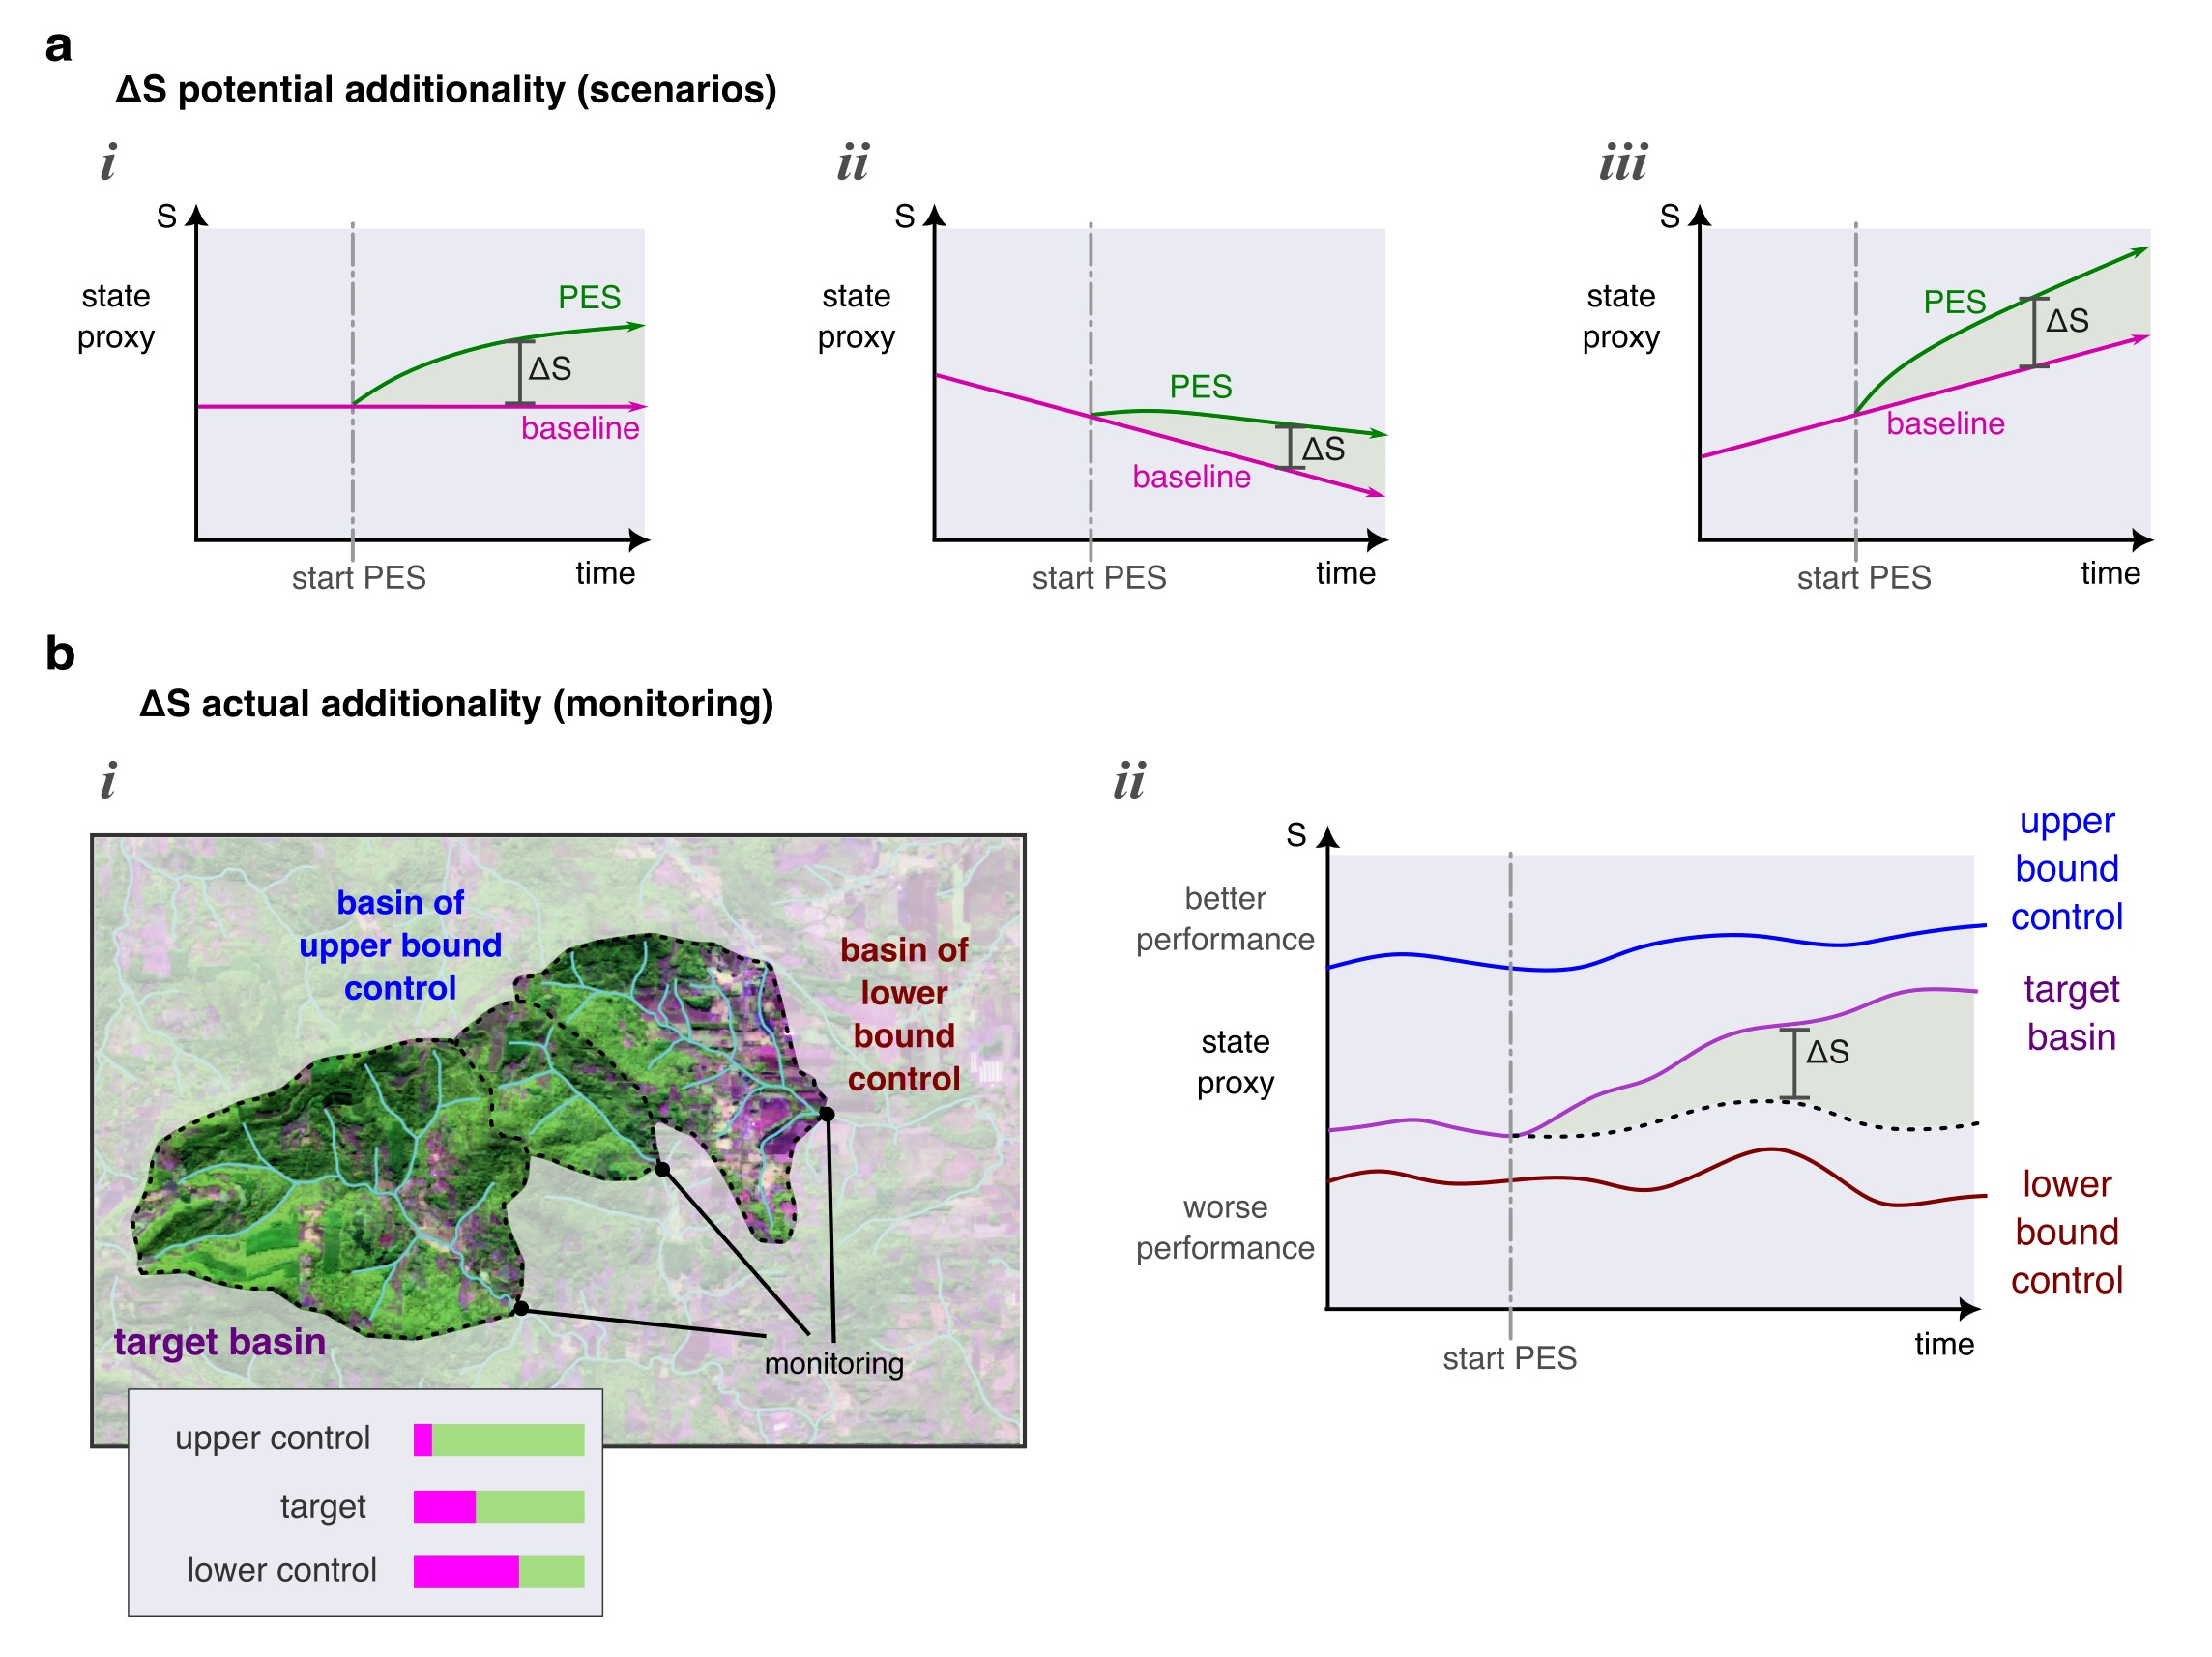
\includegraphics[width=0.98\linewidth]{figs/fig_add_en.jpg}		
\caption[Potential and actual additionality.]
{\textbf{---\;Potential and actual additionality.}
    The additionality principle aims to ensure that economic incentives yield benefits that would not occur without PES.
    \;\textbf{a}\;---\;In the planning phase of a PES scheme, efforts should be made to estimate potential additionality $\Delta S$, calculated as the difference between a state indicator $S$ in scenarios with and without PES. Scenarios can be stationary (detail \textrm{\textit{i}}), unfavorable (detail \textrm{\textit{ii}}), and favorable (detail \textrm{\textit{iii}}). The scenario without PES serves as a baseline for comparison. In practice, one approach is to compare the current scenario (without PES) to a potential native vegetation scenario (100% conservation). Such evaluations support cost-benefit analysis, coupled with valuation methods.    
    \;\textbf{b}\;---\;In the operational phase of a PES scheme, actual additionality should be measured through monitoring. In watershed PES schemes, in particular, efforts should be made to isolate causality from exogenous variables. For example, paired watersheds near the target basin can be selected as controls (detail \textrm{\textit{i}}). More degraded watersheds serve as a lower control, while better-preserved watersheds serve as an upper control (detail \textrm{\textit{ii}}).    
}
\label{fig:eco:add} 		
\end{figure}

As mentioned above, the additionality principle aims to ensure that economic incentives yield benefits that would not occur \textit{without} PES. Although this may seem evident, it was not the case in many planning studies involving hydrological models, as noted by Lele’s review (2009) \cite{Lele2009a}. Lele identified a lack of a shared, rigorous methodological framework across the modeling and valuation extremes, particularly regarding evaluations under alternative land-use scenarios. Such methodological weaknesses prompted Sven Wunder (2005, 2007) \cite{Wunder2005a, Wunder2007a} to put forth pioneering considerations on this principle. Observing additionality requires assessing natural service indicators relative to a \textbf{baseline scenario}, which serves as a comparison reference for quantifying the natural service supply capacity. This principle can support the viability of a PES scheme even under unfavorable absolute conditions. For example, even if rainfall in a basin decreases due to climate change, expanding green infrastructure may still result in a comparatively less severe future scenario. Additionality is, therefore, the \textit{difference} between the state indicator under current conditions and the state indicator in baseline conditions:
\begin{linenomath*}
\begin{equation}
\label{eq:additionality}
\Delta\text{S}_{t} = \text{S}_{t} - \text{S}_{t^*} \quad \; \forall t 
\end{equation}
\end{linenomath*}
\noindent where $\Delta\text{S}_{t}$ is the additionality at time $t$; $\text{S}_{t}$ is the natural service state indicator at time $t$; and $\text{S}_{t^*}$ is the natural service state indicator at time $t^*$, the time in the baseline scenario. Estimating \textbf{potential additionality} in planning studies is the first step in justifying the implementation of a PES scheme, as well as providing the foundation for mapping and prioritizing \textbf{priority areas}. The second step, proposed by Kroeger \textit{et al.} (2013, 2019) \cite{Kroeger2013a, Kroeger2019a}, involves integrating with valuation methods to support cost-benefit analysis and investment returns. In this regard, the exploration of future scenarios conducted by Possantti \& Marques (2022) \cite{Possantti2022a} demonstrates that this analytical approach is complex, relying heavily on auxiliary hypotheses, especially when estimating the expansion costs of NBS and the avoided costs verified downstream (see Highlight \ref{box:dp} in Chapter 2).

In watershed PES schemes, using hydrological models becomes essential for estimating potential additionality, as it is necessary to simulate the watershed's hydrological performance under alternative boundary condition scenarios, comparing results with and without planned actions (for example: Ullrich \& Volk, 2009; Carvalho-Santos \textit{et al.}, 2014; Martinez-Martinez \textit{et al.}, 2014; Daneshi \textit{et al.}, 2021 \cite{Ullrich2009a, Carvalho-santos2014a, Martinez-martinez2014a, Daneshi2021a}). However, this evaluation is only feasible when applying conceptual models that explicitly represent various hydrological processes in zero-order watersheds. Data-driven models, regardless of their predictive capacity, are not applicable in such cases, as they do not permit deductive inference about scenarios. A key methodological decision, however, is defining the baseline scenario. Following a natural services restoration logic, the strategy proposed by Lima \textit{et al.} (2017) \cite{Lima2017} involves defining this scenario based on \textbf{potential native vegetation}, that is, a land cover scenario representing natural vegetation development without anthropic changes. In this context, potential additionality equates to \textbf{hydrological anomaly} since it refers to the hydrological disturbance caused by current anthropic activities, such as agriculture and urbanization. This approach is straightforward and evidence-based, as the posterior distribution of hydrological parameters associated with potential native vegetation is estimable in well-preserved watersheds. However, it does not provide a means to estimate additionality for other land cover types seeking good hydrological performance, like NBS, but with parameters that are not readily estimable based on empirical evidence.

The additionality principle should not, however, be limited to the planning phase; it should also be present in the continuous operation and management of a PES program. Thus, beyond potential additionality, it is essential to estimate \textbf{actual additionality} over time, enabling dynamic adaptation and course correction. Therefore, it is necessary to establish and monitor state indicators of the target service that demonstrate actual additionality. Ideally, these indicators are the hydrological variables that represent the underlying processes, such as baseflow, but can also include indirect and complementary metrics, such as land cover and land use, which can be monitored at a lower cost via remote sensing. An example of actual additionality monitoring is presented by Sone \textit{et al.} (2019) \cite{Sone2019a}, where the authors evaluated whether a watershed PES program in the Guariroba River Basin in central Brazil produced observable impacts. In the study, precipitation and flow were monitored from 2012 to 2016, during which soil and water conservation practices, such as contour terrace construction and riparian vegetation restoration, were implemented. The results, combined with trend analysis of time series, showed that while precipitation records exhibited a downward trend (1 mm per month), baseflow increased by 18 liters per second during the monitoring period. Such field observations reinforce the need to check not only target service indicators but also exogenous variables that create \textit{extenuating circumstances}, like precipitation. If precipitation had \textit{increased} during the monitoring period, Sone \textit{et al.} (2019) would not have been as confident in asserting the actual additionality of the actions. In this regard, an ideal monitoring system in a watershed PES scheme should adopt a \textbf{paired watersheds} approach, where \textbf{control watersheds} where \textit{no} actions are taken are also monitored. More degraded control watersheds thus provide a \textbf{real baseline}, while more preserved control watersheds offer a \textbf{real ceiling}. A monitoring system of this scale naturally consumes program financial resources, encouraging the exploration of less conventional strategies, such as using \textbf{bioindicators} -- algae, plankton, and lotic ecosystem invertebrates. These organisms, as they reflect multiple aspects of ecological structure, can be periodically sampled, providing information on the recent history of environmental conditions. This approach allows ecosystem changes to be identified more economically and complements hydrological variables, offering an integrated view of conservation practices’ impacts over time.

\subsection{Applications with the \texttt{PLANS} model}

\begin{figure}[t!] 
\centering				
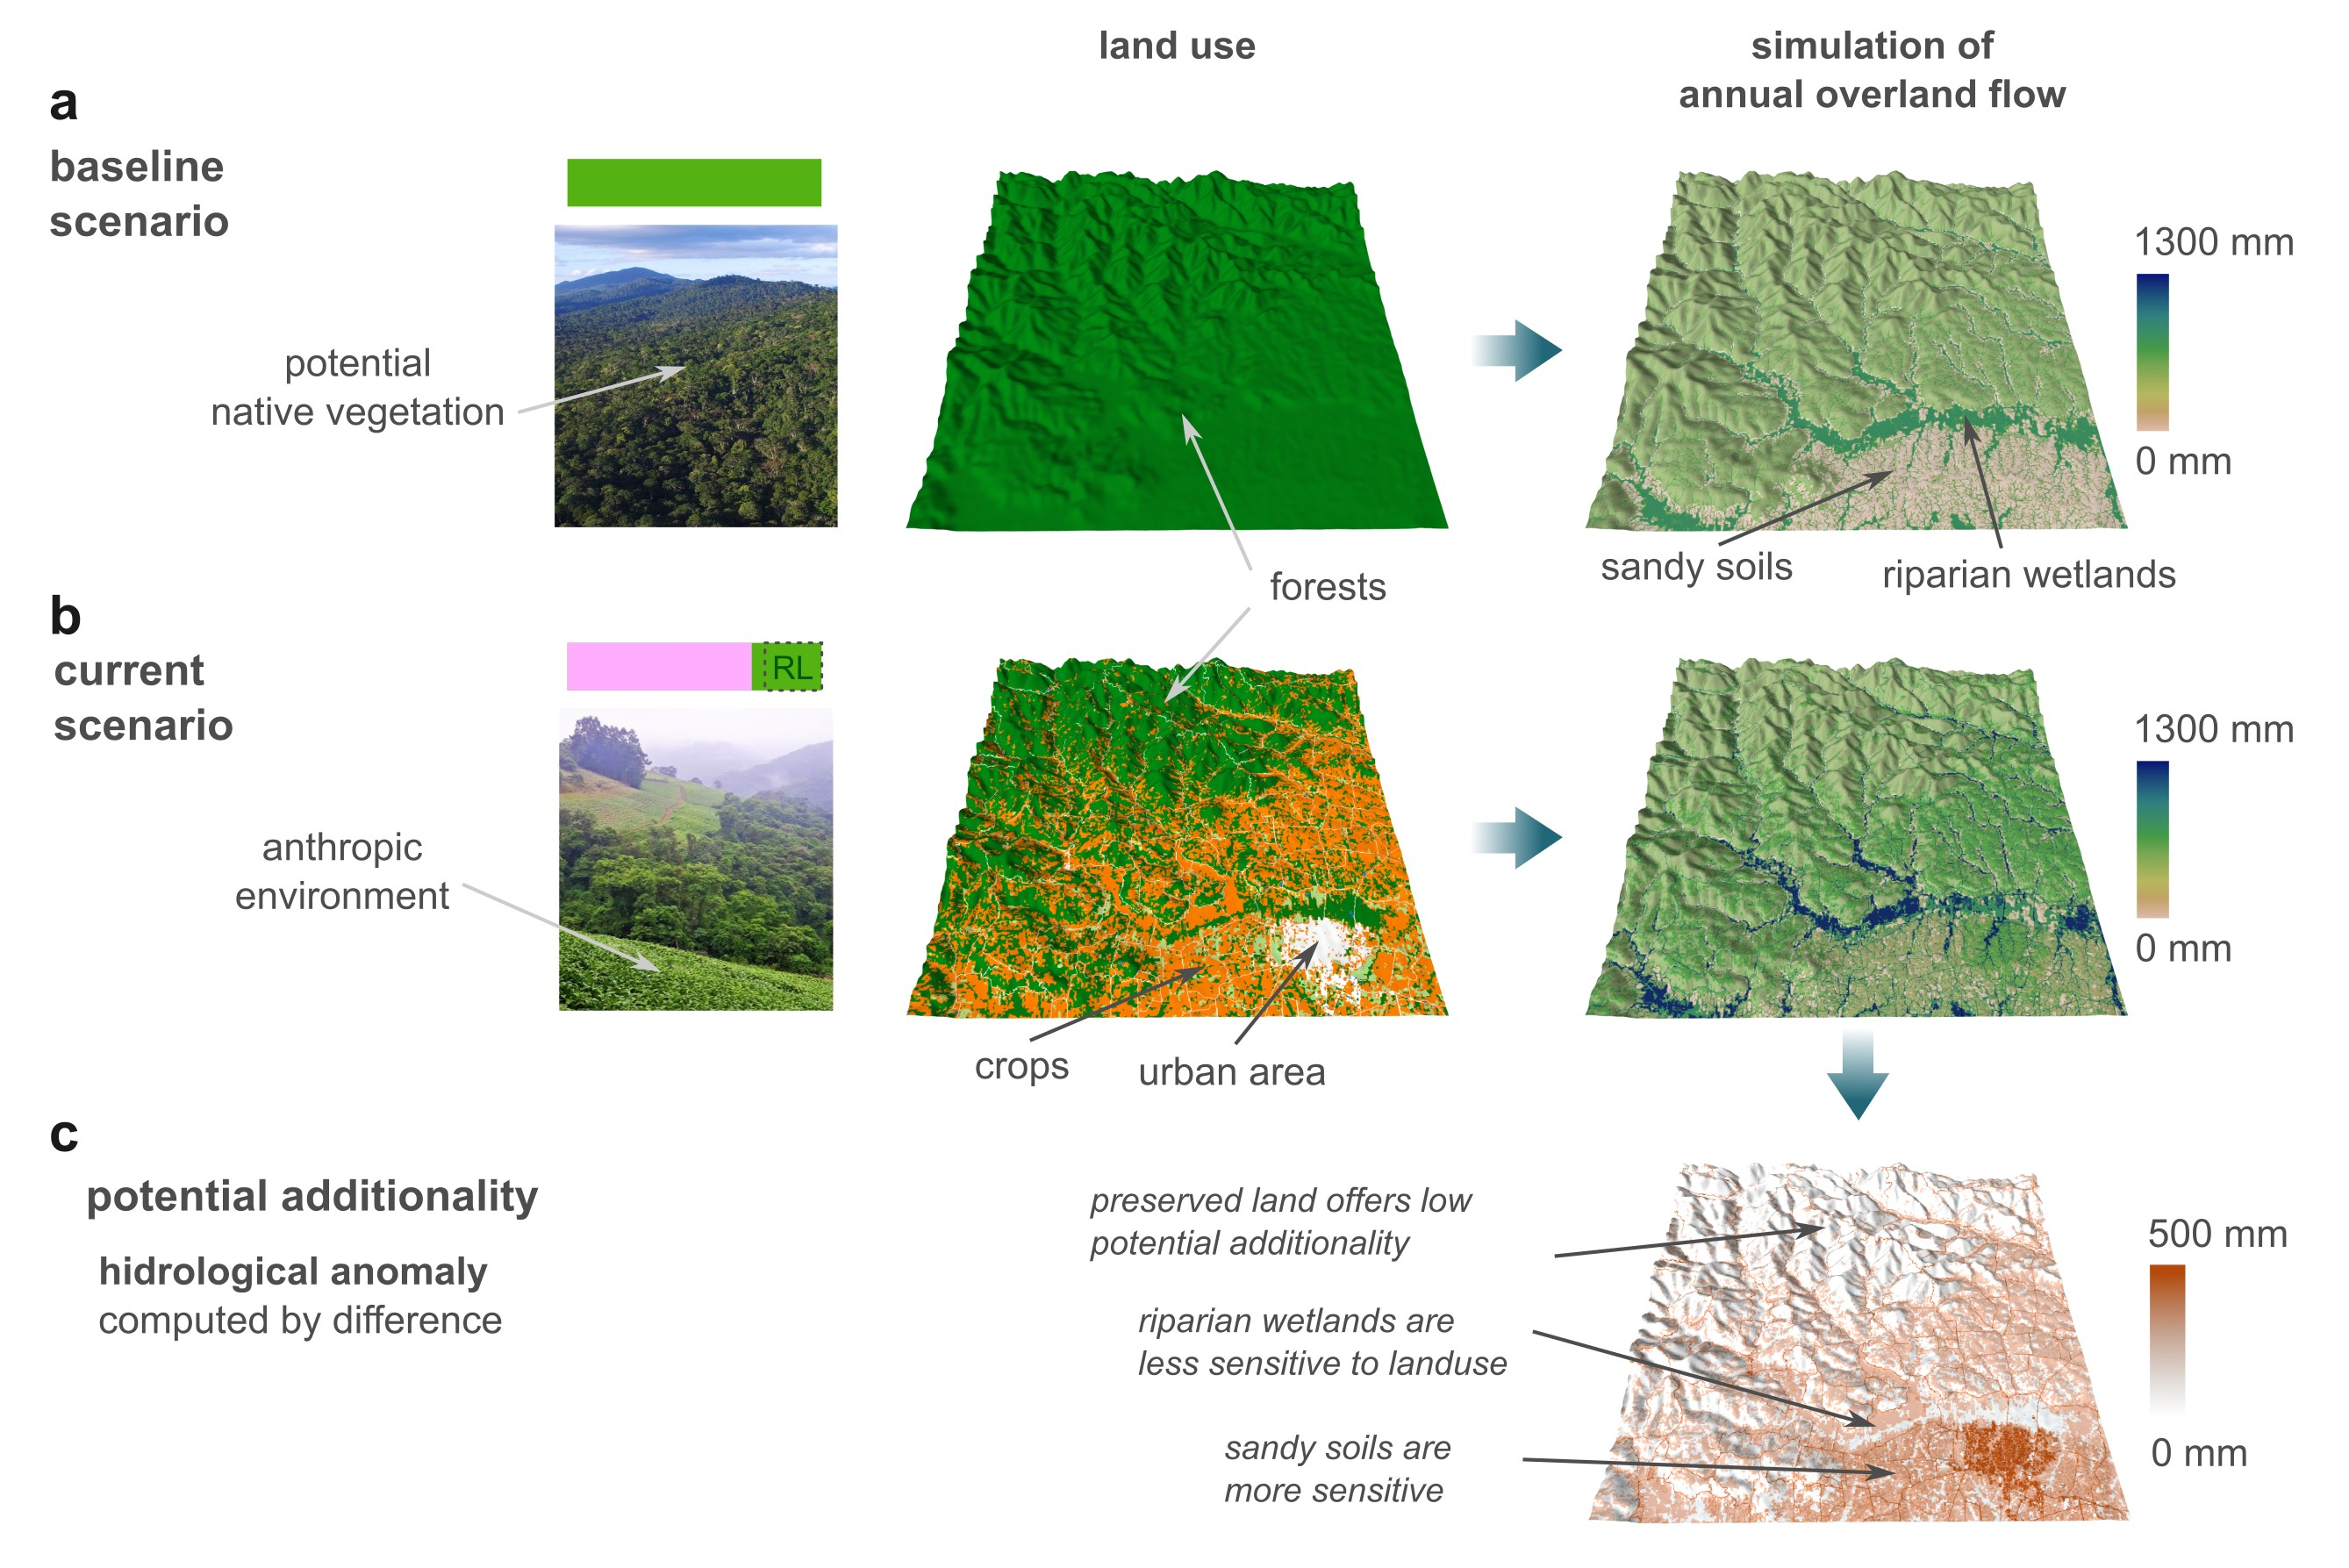
\includegraphics[width=0.98\linewidth]{figs/fig_addplans_en.jpg}		
\caption[Potential additionality with the PLANS model]
{\textbf{---\;Estimating potential additionality with the PLANS model.}
    With the PLANS model, it is possible to estimate potential additionality by simulating watershed hydrology under alternative land-use scenarios. Based on TOPMODEL, it considers not only soils and cover but also the dynamic influence of topography and riparian wetlands, which distinguishes it from other models. This example illustrates the results for the Arroio Castelhano watershed in Venâncio Aires, RS. Daily surface runoff maps from 10 years of simulations were annualized and compared.    
    \;\textbf{a}\;---\;Baseline scenario configured as potential native vegetation. In this uniform land-cover scenario, areas with sandy soils produce naturally less surface runoff due to hydraulic conductivity, while riparian wetlands naturally produce more runoff due to topography.
    \;\textbf{b}\;---\;Current land-cover scenario, with mosaics of cities, roads, and croplands, highlights increased surface runoff across the entire basin, primarily due to reduced infiltration capacity.    
    \;\textbf{c}\;---\;The difference between scenarios then demonstrates the sensitivity of each landscape area, showing that already preserved areas offer no additionality. Likewise, riparian wetlands offer little additionality. Cropland areas with sandy soils, however, are far more sensitive, attracting action prioritization.
}
\label{fig:eco:addplans1} 		
\end{figure}

The \texttt{PLANS} model, developed collaboratively with colleagues (see Section \ref{sec:hydro:plans}), emerges as an alternative to the widely-used \texttt{SWAT} and \texttt{InVEST} models for modeling watershed natural services (Francesconi \textit{et al.}, 2016 \cite{Francesconi2016}; Possantti \textit{et al.}, 2023 \cite{Possantti2023a}). The \texttt{SWAT} model simulates multiple hydrological processes by considering hydrological response units, drainage networks, and sub-watersheds \cite{Strauch2013}. In contrast, \texttt{InVEST}, particularly in its water balance module, utilizes high spatial resolution maps, though processes are simplified to an annual scale \cite{Daneshi2021a}. While \texttt{SWAT} provides greater conceptual detail of processes, \texttt{InVEST} offers finer spatial resolution \cite{Cong2020a}. The \texttt{PLANS} model combines these attributes: conceptual detail and high spatial resolution, achieved by expanding the classic \texttt{TOPMODEL} version, which defines hydrological response units based on topographical attributes, lending detailed spatial nuances to the model.

\begin{figure}[t!] 
\centering				
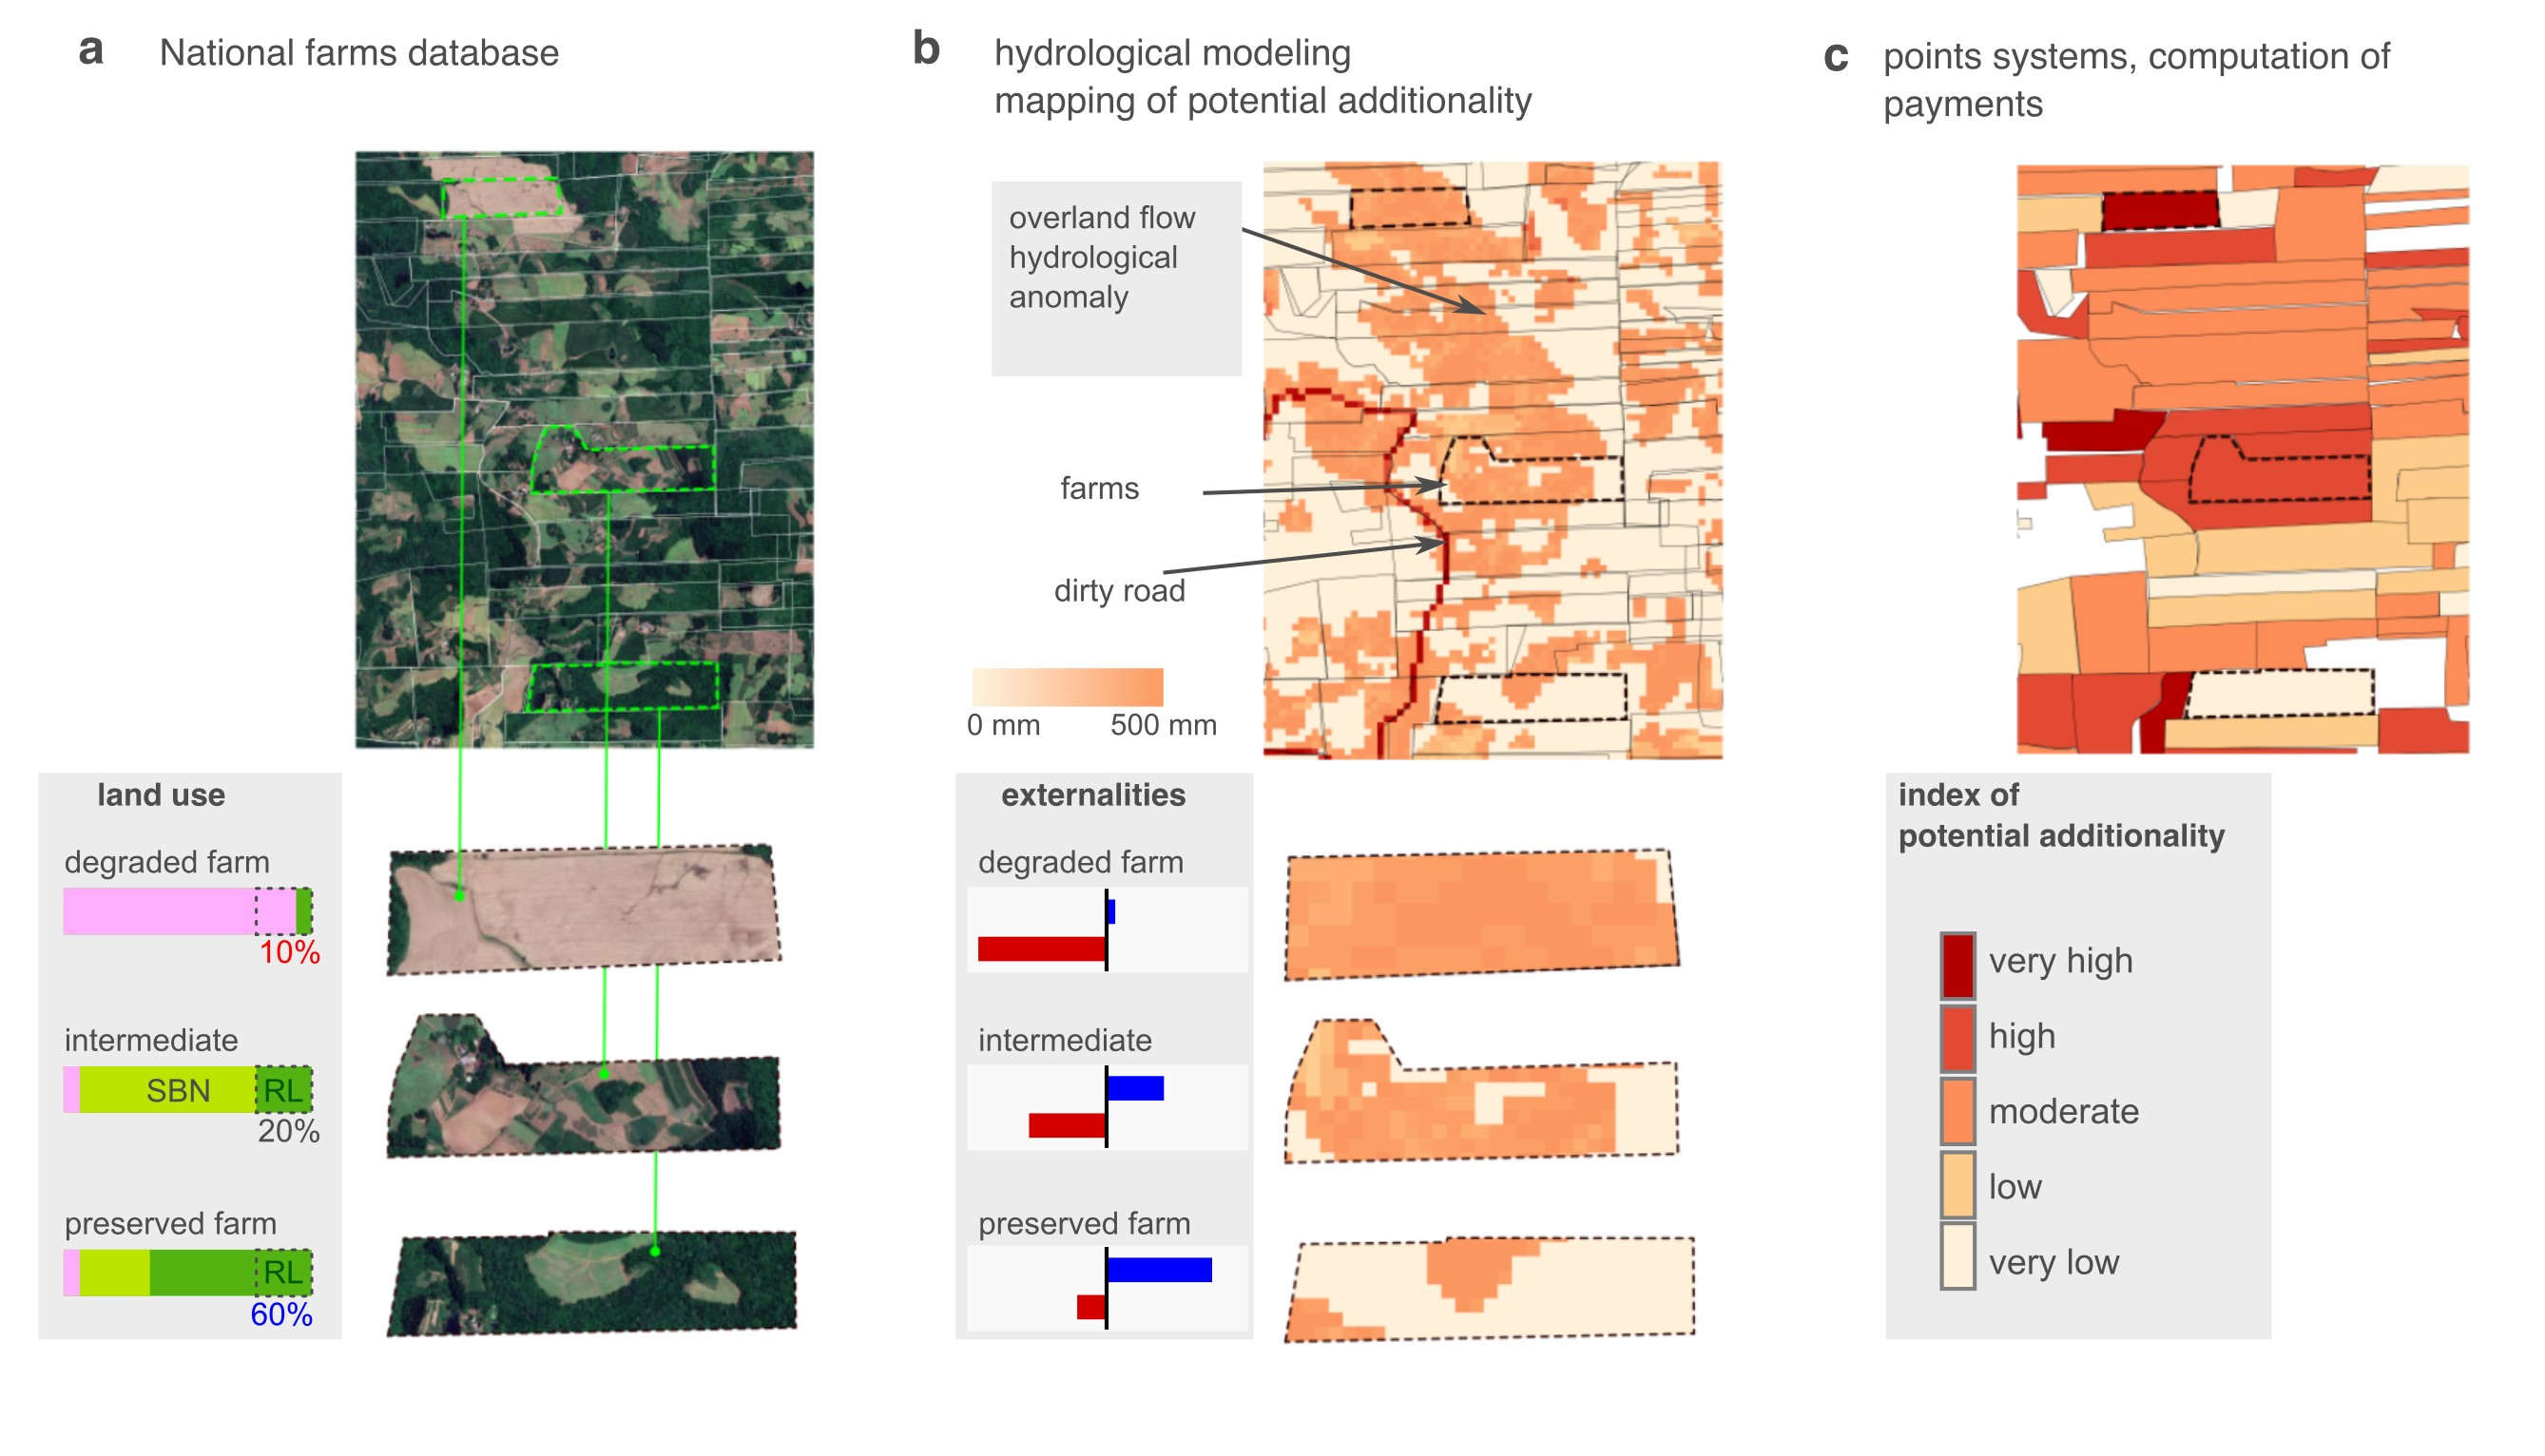
\includegraphics[width=0.98\linewidth]{figs/fig_lotscale_en.jpg}		
\caption[Additionality at the operational lot scale]
{\textbf{---\;Evaluating potential additionality at the operational scale of lots.}
    Another unique aspect of the PLANS model is its capacity to produce high spatial resolution results, facilitating potential additionality estimates at the operational scale of rural lots. This advantage stems primarily from its organization into hydrological response units more detailed than conventional models. 
    \;\textbf{a}\;---\;The Rural Environmental Registry provides the territorial division of rural lots, including the individual property plan. Combined with high-resolution remote sensing, it is possible to discern more or less degraded lots.    
    \;\textbf{b}\;---\;PLANS model results help estimate each lot's potential additionality, providing insight into the magnitude of each lot's negative externality for downstream.    
    \;\textbf{c}\;---\;Each lot's potential additionality can then be aggregated into priority indices, aiding planning actions in PES schemes.
}
\label{fig:eco:addplans2} 		
\end{figure}

Regarding potential additionality mapping, illustrated in Figure \ref{fig:eco:addplans1}, PLANS land-cover scenario simulations in the Arroio Castelhano watershed (383 km²) in Venâncio Aires estimated an average surface runoff reduction capacity of around 20\% (200 mm/year) and an increase in baseflow of approximately 25\% (80 mm/year), meaning roughly a thousand liters per second of cleaner, relatively perennial water in the watercourse. Annualized maps show hydrological anomaly patterns, especially in anthropized areas where land cover has a greater influence. In the mountainous headwaters and more preserved Atlantic Forest areas, the anomaly is lower or even nonexistent. Among anthropized areas, one sandy-soil region demonstrated greater sensitivity, as surface runoff was nearly absent in the reference conditions due to high soil hydraulic conductivity. Additionally, the model showed that in thalweg and riparian wetland areas, where topography is more influential, hydrological anomalies are relatively lower. In these locations, surface runoff generation is less dependent on land cover and use, whether natural or anthropized. This sensitivity is not captured in hydrological models like \texttt{SWAT} and \texttt{InVEST}, which do not represent the variable contributing area phenomenon.

On the spatial resolution side, the \texttt{PLANS} model enables potential additionality assessment within each rural lot, i.e., at the operational scale suitable for differentiating among lots. This advantage results from representing topographical influence, which allows the precise spatial reconstruction of simulated hydrological process maps. Therefore, rural lots with the same soil type and cover class, but located in different parts of the landscape (e.g., hillside and floodplain), may exhibit distinct potential additionalities, depending on the predominant runoff generation mechanisms. It is worth noting that rural lot boundaries, available from the Rural Environmental Registry, are an essential data source for developing Individual Property Plans (PIP), applicable in both PES programs and command-and-control contexts, such as enforcing Forest Code regulations. Integrating with this registry in potential additionality modeling is thus a notable advantage of the \texttt{PLANS} model for mapping priority areas and objectively scoring candidate lots in PES calculators, also observing the transparency principle. Detailed maps showing rural lots and their various environmental attributes, including hydrological ones, strengthen trust among all parties involved.

\begin{figure}[t!] 
\centering				
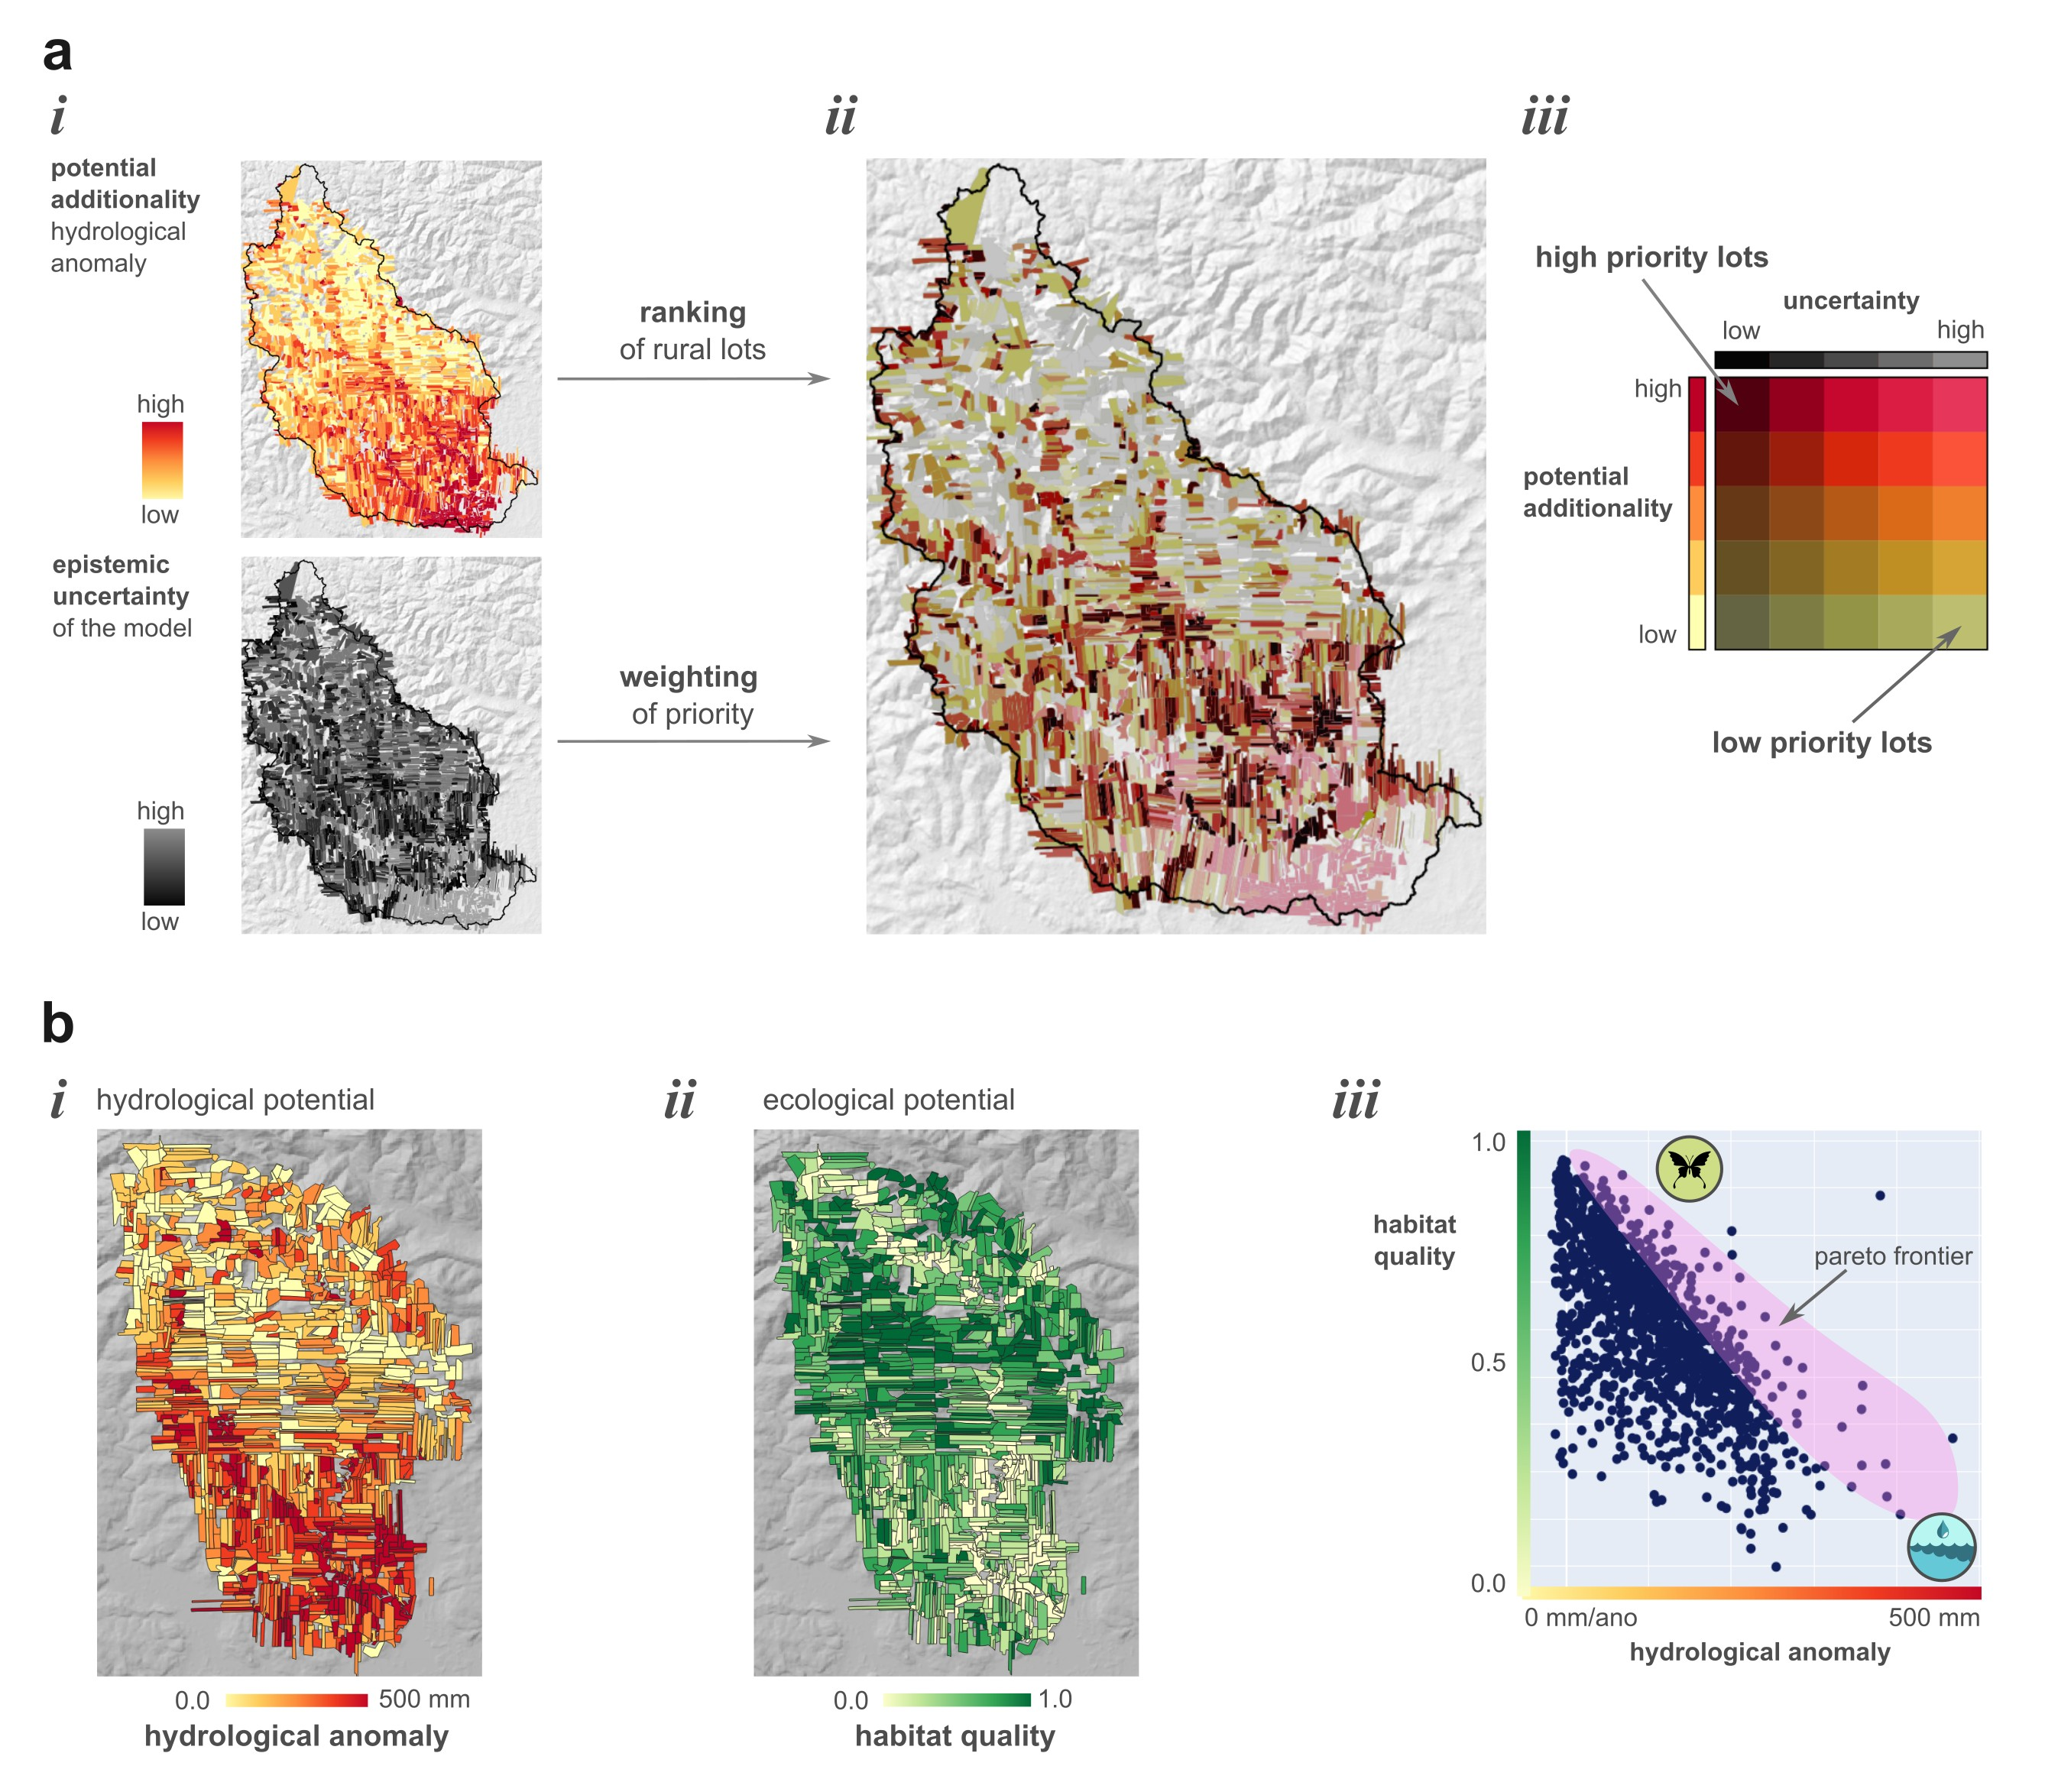
\includegraphics[width=0.98\linewidth]{figs/fig_index_en.jpg}		
\caption[Priority index and trade-offs]
{\textbf{---\;Priority index and trade-off assessment.}
    Applications with the PLANS model open pathways for incorporating uncertainties and evaluating trade-offs.
    \;\textbf{a}\;---\;A priority index for rural lots based on models like PLANS should consider the spatial uncertainties of simulations (detail \textrm{\textit{i}}). Spatial uncertainty bands, thus, act as weighting factors for ranking, producing a priority index (detail \textrm{\textit{ii}}) that reflects both performance attractiveness (higher potential additionality) and estimation reliability (lower uncertainty, detail \textrm{\textit{iii}}).   
    \;\textbf{b}\;---\;Results from ecological models like the Habitat Quality model in \texttt{InVEST} can be integrated into a comprehensive analysis that considers synergies and trade-offs. In the Arroio Grande watershed example (Venâncio Aires), potential hydrological additionality emerged in lower watershed areas, where rural lots are more degraded. On the other hand, habitat quality offers ecological additionality potential, as it is more worthwhile to restore ecosystem fragments where preservation is already higher. This dichotomy in priorities results in a trade-off analysis where the best lots are located on a pareto frontier.
}
\label{fig:eco:addplans3} 		
\end{figure}

Finally, applying the \texttt{PLANS} model in the Arroio Castelhano watershed incorporated the inherent uncertainties of hydrological modeling (detailed in Chapter 1; see Highlight \ref{box:uncert}). To do this, the priority index construction included weighting by the dispersion of empirically adequate models generated by the GLUE method, in combination with a search algorithm (see Highlight \ref{box:glue} for more information). Thus, priority lots are defined as those with the highest potential additionality and the lowest associated uncertainty. This approach also opens new paths, such as trade-off and multiple-target service evaluations, as recommended by Naeem \textit{et al.} (2015). For example, Figure \ref{fig:eco:addplans3} also shows an assessment between potential hydrological and ecological additionality. Generally, these two indicators do not coincide, forming a \textbf{pareto frontier} between services. This occurs because, in ecological terms, potential additionality is higher where native ecosystem fragmentation is lower, favoring priority actions on \textit{better-preserved} lots than degraded ones, as in the hydrological potential case. With these contributions, the \texttt{PLANS} model seeks to integrate hydrological modeling from its most philosophical foundations to its most operational consequences, providing a robust and scientifically rigorous methodological framework to guide the transition to sustainable development in the coming decades. $\blacksquare$


\clearpage

\section{Chapter summary}

\par In this chapter, I address the application of ecological economic principles to watershed management, advocating for a paradigm shift that sees watersheds not merely as exploitable resources but as integral components of natural capital with inherent limits. The discussion centers on the sustainable balance of resource use, emphasizing the essential role of natural services, especially watershed services, in supporting both human well-being. By adopting economic valuation methods and promoting the use of land use economic instruments like Payment for Ecosystem Services (PES), this chapter aims to outline strategies for enhancing watershed management while highlighting the importance of scientific rigor in environmental planning.

\begin{itemize}
    
    \item[$\blacksquare$] \textbf{Ecology implies a finite world.} The ecological economics model is introduced as a departure from traditional economic paradigms, emphasizing that nature should not only be viewed as a resource to exploit but as natural capital with inherent limits. Unlike neoclassical economics, which often neglects these boundaries, ecological economics places ecological sustainability at the forefront, encouraging strategies that maintain ecosystem functions while supporting human well-being. This approach includes the recognition of externalities, especially in watershed contexts where upstream land users impact downstream water users.
    
    \item[$\blacksquare$] \textbf{Natural capital implies an optimal scale.} Natural capital, such as forests in watersheds, is positioned as essential for providing natural services that support human life. The chapter argues that there is an optimal scale of resource use that ensures the regeneration of natural capital. When applied to watersheds, this concept urges a balance between water use for agriculture, urban needs, and conservation. Overstepping these natural limits risks degrading the ecosystem’s ability to provide services like clean water, flood control, and sediment retention.
    
    \item[$\blacksquare$] \textbf{Escaping the tragedy.} Common goods, as open-access resources, are vulnerable to overuse and degradation—a dynamic described as \textit{the tragedy of the commons}. In a watershed, upstream practices (e.g., deforestation, pollution) can create negative externalities for downstream users, leading to conflicts and degradation. Economic instruments like watershed PES programs can help advance conservation in upstream areas beyond the mandatory law, thereby protecting water quality and availability for downstream communities.
    
    \item[$\blacksquare$] \textbf{Natural accounting.} Using frameworks like the Common International Classification of Ecosystem Services (CICES) and the Economics of Ecosystems and Biodiversity (TEEB) allows for the systematic categorization and valuation of natural services. Watershed services are broken down into provisioning, regulating, and cultural sections, each with distinct utilitarian values. Valuation methods are emphasized as tools to demonstrate the economic importance of watershed services, providing stakeholders with information for decision-making and fostering public and private support for conservation efforts.
    
    \item[$\blacksquare$] \textbf{The application of scientific guidelines.} Among others, the principle of additionality is central to PES programs, ensuring that incentives lead to environmental benefits beyond what would occur without intervention. By comparing scenarios with and without conservation practices, potential additionality quantifies the impact of PES in the planning phase, ensuring transparency and effectiveness in achieving conservation goals. Explicit and measurable metrics allow the monitoring of processes to infer the actual additionality during the operational phase.
    
    \item[$\blacksquare$] \textbf{Advantages of the PLANS model.} The PLANS model, based on TOPMODEL, is highlighted for its capability to simulate watershed processes with spatial detail, incorporating topographic, soil, and land cover data. This high-resolution approach allows PLANS to assess additionality at the plot level, aiding in prioritizing areas for conservation. Unlike other models, PLANS integrates both conceptual detail and spatial accuracy, providing nuanced insights into the impacts of land-use changes, evaluating trade-offs, and assessing uncertainty, enabling better-targeted conservation actions within PES programs.
    
\end{itemize}


\end{document}